\documentclass[12pt,]{book}
\usepackage{lmodern}
\usepackage{setspace}
\setstretch{1.5}
\usepackage{amssymb,amsmath}
\usepackage{ifxetex,ifluatex}
\usepackage{fixltx2e} % provides \textsubscript
\ifnum 0\ifxetex 1\fi\ifluatex 1\fi=0 % if pdftex
  \usepackage[T1]{fontenc}
  \usepackage[utf8]{inputenc}
\else % if luatex or xelatex
  \ifxetex
    \usepackage{mathspec}
  \else
    \usepackage{fontspec}
  \fi
  \defaultfontfeatures{Ligatures=TeX,Scale=MatchLowercase}
\fi
% use upquote if available, for straight quotes in verbatim environments
\IfFileExists{upquote.sty}{\usepackage{upquote}}{}
% use microtype if available
\IfFileExists{microtype.sty}{%
\usepackage{microtype}
\UseMicrotypeSet[protrusion]{basicmath} % disable protrusion for tt fonts
}{}
\usepackage[margin=1in]{geometry}
\usepackage{hyperref}
\hypersetup{unicode=true,
            pdftitle={Data Science Workshop},
            pdfauthor={Alistair Bailey},
            pdfborder={0 0 0},
            breaklinks=true}
\urlstyle{same}  % don't use monospace font for urls
\usepackage{natbib}
\bibliographystyle{apalike}
\usepackage{color}
\usepackage{fancyvrb}
\newcommand{\VerbBar}{|}
\newcommand{\VERB}{\Verb[commandchars=\\\{\}]}
\DefineVerbatimEnvironment{Highlighting}{Verbatim}{commandchars=\\\{\}}
% Add ',fontsize=\small' for more characters per line
\usepackage{framed}
\definecolor{shadecolor}{RGB}{248,248,248}
\newenvironment{Shaded}{\begin{snugshade}}{\end{snugshade}}
\newcommand{\AlertTok}[1]{\textcolor[rgb]{0.94,0.16,0.16}{#1}}
\newcommand{\AnnotationTok}[1]{\textcolor[rgb]{0.56,0.35,0.01}{\textbf{\textit{#1}}}}
\newcommand{\AttributeTok}[1]{\textcolor[rgb]{0.77,0.63,0.00}{#1}}
\newcommand{\BaseNTok}[1]{\textcolor[rgb]{0.00,0.00,0.81}{#1}}
\newcommand{\BuiltInTok}[1]{#1}
\newcommand{\CharTok}[1]{\textcolor[rgb]{0.31,0.60,0.02}{#1}}
\newcommand{\CommentTok}[1]{\textcolor[rgb]{0.56,0.35,0.01}{\textit{#1}}}
\newcommand{\CommentVarTok}[1]{\textcolor[rgb]{0.56,0.35,0.01}{\textbf{\textit{#1}}}}
\newcommand{\ConstantTok}[1]{\textcolor[rgb]{0.00,0.00,0.00}{#1}}
\newcommand{\ControlFlowTok}[1]{\textcolor[rgb]{0.13,0.29,0.53}{\textbf{#1}}}
\newcommand{\DataTypeTok}[1]{\textcolor[rgb]{0.13,0.29,0.53}{#1}}
\newcommand{\DecValTok}[1]{\textcolor[rgb]{0.00,0.00,0.81}{#1}}
\newcommand{\DocumentationTok}[1]{\textcolor[rgb]{0.56,0.35,0.01}{\textbf{\textit{#1}}}}
\newcommand{\ErrorTok}[1]{\textcolor[rgb]{0.64,0.00,0.00}{\textbf{#1}}}
\newcommand{\ExtensionTok}[1]{#1}
\newcommand{\FloatTok}[1]{\textcolor[rgb]{0.00,0.00,0.81}{#1}}
\newcommand{\FunctionTok}[1]{\textcolor[rgb]{0.00,0.00,0.00}{#1}}
\newcommand{\ImportTok}[1]{#1}
\newcommand{\InformationTok}[1]{\textcolor[rgb]{0.56,0.35,0.01}{\textbf{\textit{#1}}}}
\newcommand{\KeywordTok}[1]{\textcolor[rgb]{0.13,0.29,0.53}{\textbf{#1}}}
\newcommand{\NormalTok}[1]{#1}
\newcommand{\OperatorTok}[1]{\textcolor[rgb]{0.81,0.36,0.00}{\textbf{#1}}}
\newcommand{\OtherTok}[1]{\textcolor[rgb]{0.56,0.35,0.01}{#1}}
\newcommand{\PreprocessorTok}[1]{\textcolor[rgb]{0.56,0.35,0.01}{\textit{#1}}}
\newcommand{\RegionMarkerTok}[1]{#1}
\newcommand{\SpecialCharTok}[1]{\textcolor[rgb]{0.00,0.00,0.00}{#1}}
\newcommand{\SpecialStringTok}[1]{\textcolor[rgb]{0.31,0.60,0.02}{#1}}
\newcommand{\StringTok}[1]{\textcolor[rgb]{0.31,0.60,0.02}{#1}}
\newcommand{\VariableTok}[1]{\textcolor[rgb]{0.00,0.00,0.00}{#1}}
\newcommand{\VerbatimStringTok}[1]{\textcolor[rgb]{0.31,0.60,0.02}{#1}}
\newcommand{\WarningTok}[1]{\textcolor[rgb]{0.56,0.35,0.01}{\textbf{\textit{#1}}}}
\usepackage{longtable,booktabs}
\usepackage{graphicx,grffile}
\makeatletter
\def\maxwidth{\ifdim\Gin@nat@width>\linewidth\linewidth\else\Gin@nat@width\fi}
\def\maxheight{\ifdim\Gin@nat@height>\textheight\textheight\else\Gin@nat@height\fi}
\makeatother
% Scale images if necessary, so that they will not overflow the page
% margins by default, and it is still possible to overwrite the defaults
% using explicit options in \includegraphics[width, height, ...]{}
\setkeys{Gin}{width=\maxwidth,height=\maxheight,keepaspectratio}
\IfFileExists{parskip.sty}{%
\usepackage{parskip}
}{% else
\setlength{\parindent}{0pt}
\setlength{\parskip}{6pt plus 2pt minus 1pt}
}
\setlength{\emergencystretch}{3em}  % prevent overfull lines
\providecommand{\tightlist}{%
  \setlength{\itemsep}{0pt}\setlength{\parskip}{0pt}}
\setcounter{secnumdepth}{5}
% Redefines (sub)paragraphs to behave more like sections
\ifx\paragraph\undefined\else
\let\oldparagraph\paragraph
\renewcommand{\paragraph}[1]{\oldparagraph{#1}\mbox{}}
\fi
\ifx\subparagraph\undefined\else
\let\oldsubparagraph\subparagraph
\renewcommand{\subparagraph}[1]{\oldsubparagraph{#1}\mbox{}}
\fi

%%% Use protect on footnotes to avoid problems with footnotes in titles
\let\rmarkdownfootnote\footnote%
\def\footnote{\protect\rmarkdownfootnote}

%%% Change title format to be more compact
\usepackage{titling}

% Create subtitle command for use in maketitle
\providecommand{\subtitle}[1]{
  \posttitle{
    \begin{center}\large#1\end{center}
    }
}

\setlength{\droptitle}{-2em}

  \title{Data Science Workshop}
    \pretitle{\vspace{\droptitle}\centering\huge}
  \posttitle{\par}
  \subtitle{British Society for Proteomic Research Meeting 2018}
  \author{Alistair Bailey}
    \preauthor{\centering\large\emph}
  \postauthor{\par}
      \predate{\centering\large\emph}
  \postdate{\par}
    \date{April 17 2019}

\usepackage{booktabs}

% Preamble
\usepackage[none]{hyphenat}
\usepackage[default,osfigures,scale=0.95]{opensans} % Open sans font
\usepackage[T1]{fontenc} % Use 8-bit encoding that has 256 glyphs
\usepackage{lettrine} % The lettrine is the first enlarged letter at the beginning of the text
\raggedbottom 
\usepackage{makeidx} % These lines add bibliography to TOC
\makeindex
\usepackage[nottoc]{tocbibind}
\renewcommand{\bibname}{References} % Rename biblography as References

\begin{document}
\maketitle

{
\setcounter{tocdepth}{1}
\tableofcontents
}
\hypertarget{overview}{%
\chapter*{Overview}\label{overview}}
\addcontentsline{toc}{chapter}{Overview}

This book covers:

\begin{enumerate}
\def\labelenumi{\arabic{enumi}.}
\tightlist
\item
  An introduction to R and RStudio
\item
  An introduction to tidyverse and base R
\item
  Importing and transforming proteomics data
\item
  Visualisation of proteomics analysis
\end{enumerate}

The analysis is of an example data set of observations for 7702 proteins
from cells in three control experiments and three treatment experiments.
The observations are signal intensity measurements from the mass spectrometer.
These intensities relate the concentration of protein observed in each experiment
and under each condition. The analysis transforms the data to examine the effect of
treatment on the cellular proteome and visualise the output using a volcano
plot , a heatmap, a Venn diagram and peptide sequence logos.
Click here to download the csv file.

\hypertarget{requirements}{%
\section*{Requirements}\label{requirements}}
\addcontentsline{toc}{section}{Requirements}

An up to date version of R \citep{R-base} and RStudio
\citep{rstudioteam2018}.

If you are new to R, then the first thing
to know is that R is a programming language and RStudio is a
program for working with R called an integrated development
environment (IDE). You can use R without RStudio, but not the other way around. Further details in Chapter
\ref{r-rstudio}.

\href{https://cran.r-project.org/}{Download R here} and
\href{https://www.rstudio.com/products/rstudio/download/}{Download RStudio Desktop here}.

These materials were generated using R version 3.5.0.

Once you've installed R and RStudio, you'll also need
a few R packages. Packages are collections of \protect\hyperlink{function-anatomy}{functions}.

Open RStudio and put the code below into the \texttt{Console}
window and press \texttt{Enter} to install these three packages.

\begin{Shaded}
\begin{Highlighting}[]
\KeywordTok{install.packages}\NormalTok{(}\KeywordTok{c}\NormalTok{(}\StringTok{"plyr"}\NormalTok{,}\StringTok{"tidyverse"}\NormalTok{,}\StringTok{"gplots"}\NormalTok{,}\StringTok{"pheatmap"}\NormalTok{,}
                   \StringTok{"gridExtra"}\NormalTok{,}\StringTok{"VennDiagram"}\NormalTok{,}\StringTok{"ggseqlogo"}\NormalTok{))}
\end{Highlighting}
\end{Shaded}

\hypertarget{intro}{%
\chapter{Introduction}\label{intro}}

There are many resources for learning R on the web. Much of Chapters \ref{intro},
\ref{tidyverse}, \ref{import} and \ref{dplyr} derive from
a \href{http://www.datacarpentry.org/lessons/}{Data Carpentry lesson} using
ecological data that I have previously \href{https://southampton-rsg.github.io/2017-08-01-southampton-dc/novice/R-ecology-lesson/index.html}{reworked},
which in turn takes a lot from \href{http://r4ds.had.co.nz/}{Hadley Wickham's R for Data Science} aka \textbf{R4DS}.
Follow the links to access those materials.

Chapter \ref{transform} deals with some statistical transformations and
visualisation methods in the context of proteomics data.

Whilst finally in
Chapter \ref{going-further} there is some advice about how to build upon the
materials covered here.

In terms of philosophy:

\begin{enumerate}
\def\labelenumi{\arabic{enumi}.}
\item
  The primary motivation for using tools such as R is to get more done, in
  less time and with less pain.
\item
  And the overall aim is to \emph{understand and communicate} findings from our
  data.
\end{enumerate}



\begin{figure}

{\centering 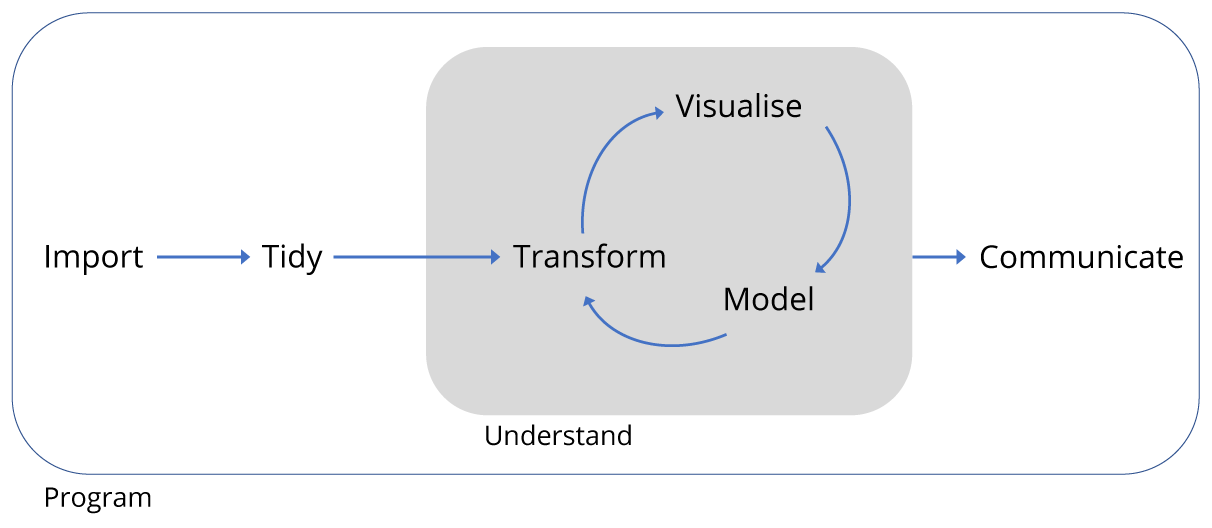
\includegraphics[width=0.8\linewidth]{img/data_project_pipeline} 

}

\caption{Data project workflow.}\label{fig:pipeline}
\end{figure}

As shown in Figure \ref{fig:pipeline} of typical data analysis workflow,
to acheive this aim we need to learn tools that enable us to perform the
fundamental tasks of tasks of importing, tidying and
often transforming the data. Transformation means for example, selecting a
subset of the data to work with, or calculating the mean of a set of observations.
We'll cover that in Chapter \ref{transform}.

But first\ldots{}

\hypertarget{r-rstudio}{%
\section{What are R and RStudio?}\label{r-rstudio}}

\textbf{\emph{``There are only two kinds of languages: the ones people complain about and the ones nobody uses''}}

\emph{Bjarne Stroustrup}

\textbf{R} is a programming language that follows the philosophy laid down by it's
predecessor S. The philosophy being that users begin in an interactive
environment where they don't consciously think of themselves as programming.
It was created in 1993, and documented in \citep{ihaka1996}.

Reasons R has become popular include that it is both open source and cross platform,
and that it has broad functionality, from the analysis of data and creating
powerful graphical visualisations and web apps.

Like all languages though it has limitations, for example the syntax is initially
confusing.

Take for example the word \texttt{environment}\ldots{}

\hypertarget{environments}{%
\subsection{Environments}\label{environments}}

An environment is where we bring our data to work with it. Here we work in a R
envrionment, using the R language as a set of tools.
\textbf{RStudio} is an integrated development environment, or IDE for R programming.
It is regularly updated, and upgrading enables access to the latest features.

The latest version can be downloaded here: \url{http://www.rstudio.com/download}

\hypertarget{why-learn-r-or-any-language}{%
\section{Why learn R, or any language ?}\label{why-learn-r-or-any-language}}

We can write R code without saving it, but it's generally more useful to write
and save our code as a script. Working with scripts makes the steps you used in
your analysis clear, and the code you write can be inspected by someone else who
can give you feedback and spot mistakes.

Learning R (or any programming language) and working with scripts forces you to
have deeper understanding of what you are doing, facilitates your learning
and comprehension of the methods you use:

\begin{itemize}
\tightlist
\item
  Writing and publishing code is important for reproducible resarch
\item
  R has many thousands of packages covering many disciplines.
\item
  R can work with many types of data.
\item
  They is a large R community for development and support.
\item
  Using R gives you control over your figures and reports.
\end{itemize}

\hypertarget{finding-your-way-around-rstudio}{%
\section{Finding your way around RStudio}\label{finding-your-way-around-rstudio}}

Let's begin by learning about \href{https://www.rstudio.com/}{RStudio}, the
Integrated Development Environment (IDE).

We will use R Studio IDE to write code, navigate the files found on our computer,
inspect the variables we are going to create, and visualize the plots we will
generate. R Studio can also be used for other things (e.g., version control,
developing packages, writing Shiny apps) that we don't have time to cover during
this workshop.

R Studio is divided into ``Panes'', see Figure \ref{fig:rstudio}.

When you first open it, there are three panes,the console where you type
commands, your environment/history (top-right), and your
files/plots/packages/help/viewer (bottom-right).

The enivronment shows all the R objects you have created or are using, such
as data you have imported.

The output pane can be used to view any plots you have created.

Not opened at first start up is the fourth default pane: the script editor pane,
but this will open as soon as we create/edit a R script (or many other document types).
\emph{The script editor is where will be typing much of the time.}



\begin{figure}

{\centering 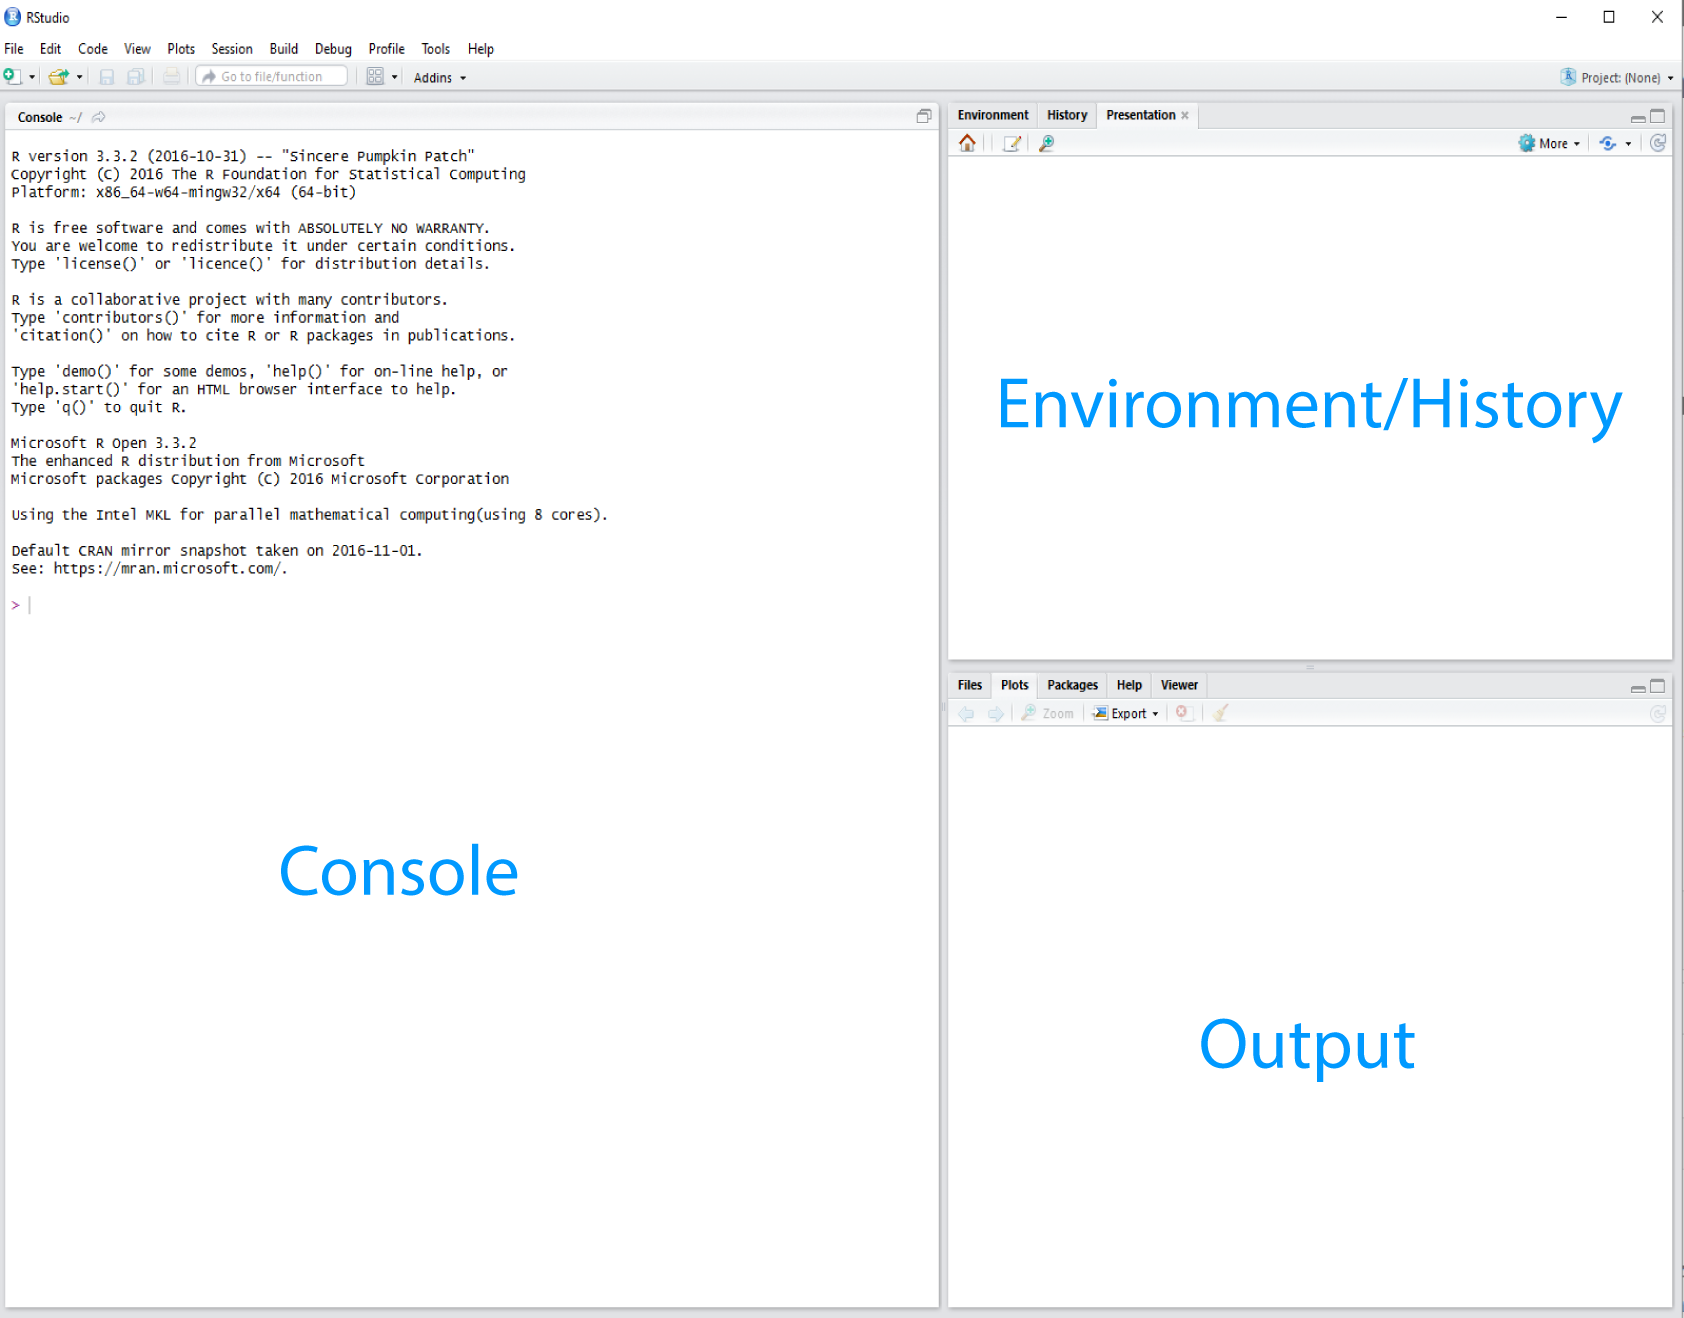
\includegraphics[width=0.8\linewidth]{img/rstudio_ide_image} 

}

\caption{The Rstudio Integrated Development Environment (IDE).}\label{fig:rstudio}
\end{figure}

The placement of these panes and their content can be customized (see menu,
R Studio -\textgreater{} Tools -\textgreater{} Global Options -\textgreater{} Pane Layout). One of the advantages of
using R Studio is that all the information you need to write code is available
ina single window. Additionally, with many shortcuts, auto-completion, and
highlighting for the major file types you use while developing in R, R Studio
will make typing easier and less error-prone.

Time for a philosphical diversion\ldots{}

\hypertarget{what-is-real}{%
\subsection{What is real?}\label{what-is-real}}

At the start, we might consider our environment ``real'' - that is to say the objects
we've created/loaded and are using are ``real''. But it's much better in the long run
to consider our scripts as ``real'' - our scripts are where we write down the code
that creates our objects that we'll be using in our environment.

\textbf{As a script is a document, it is reproducible}

Or to put it another way: we can easily recreate an environment from our scripts,
but not so easily create a script from an enivronment.

To support this notion of thinking in terms of our scripts as real, we recommend
turning off the preservation of workspaces between sessions by setting the
Tools \textgreater{} Global Options menu in R studio as shown in Figure \ref{fig:workspace}:



\begin{figure}

{\centering 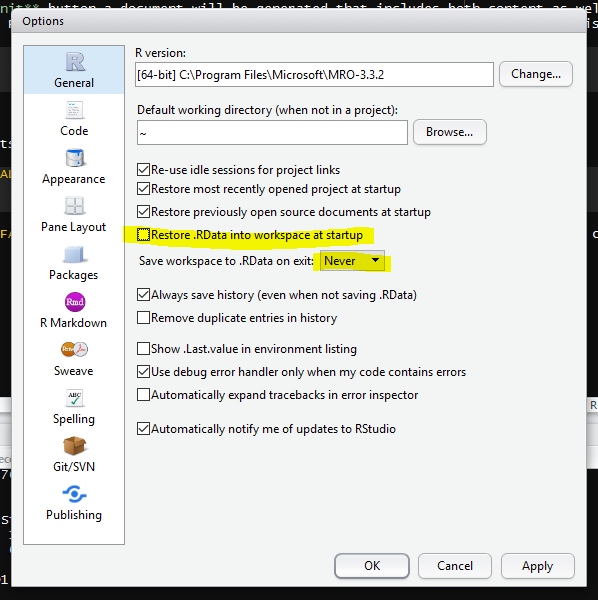
\includegraphics[width=0.8\linewidth]{img/rdata_turn_off} 

}

\caption{Don't save your workspace, save your script instead.}\label{fig:workspace}
\end{figure}

\hypertarget{where-am-i}{%
\section{Where am I?}\label{where-am-i}}

R studio tells you where you are in terms of directory address like so:



\begin{figure}

{\centering 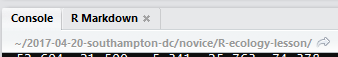
\includegraphics[width=0.8\linewidth]{img/rstudio_working_directory} 

}

\caption{Your working directory}\label{fig:working-directory}
\end{figure}

If you are unfamiliar with how computers structure folders and files, then
consider a tree with a root from which the trunk extends and branches divide.
In the image above, the \textasciitilde{} symbol represents a contraction of the path from the
root to the `home' directory (in Windows this is `Documents') and then the
forward slashes are the branches. (Note: Windows uses backslashes, Unix type
systems and R use forwardslashes).

It is good practice to keep a set of related data, analyses, and text
self-contained in a single folder, called the \textbf{working directory}. All of the
scripts within this folder can then use \emph{relative paths} to files that indicate
where inside the project a file is located (as opposed to absolute paths, which
point to where a file is on a specific computer). Working this way makes it
a lot easier to move your project around on your computer and share it with
others without worrying about whether or not the underlying scripts will still
work.



\begin{figure}

{\centering 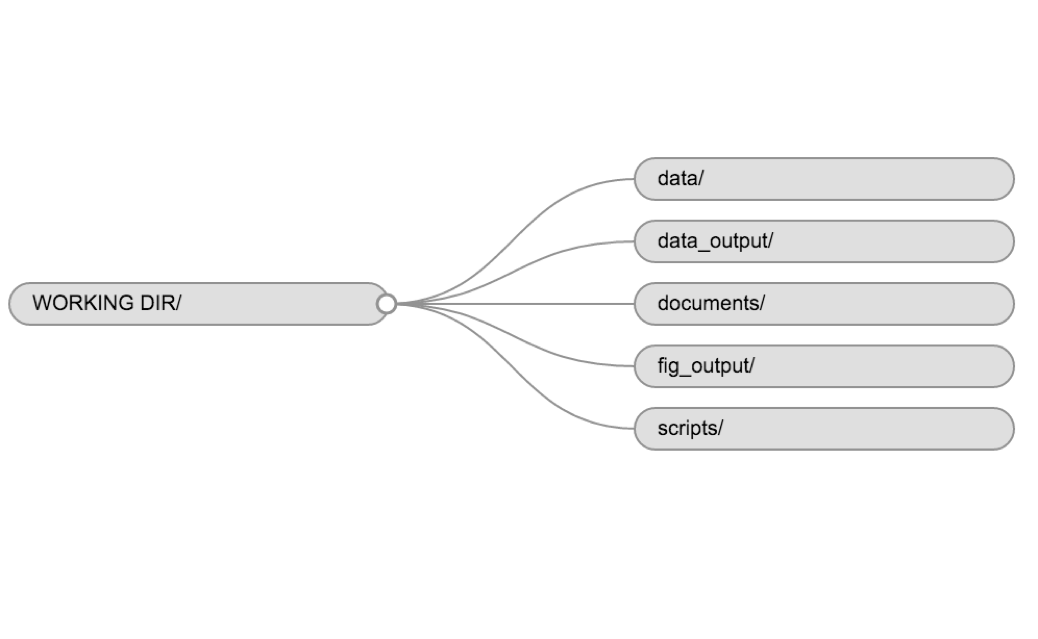
\includegraphics[width=0.8\linewidth]{img/R-ecology-work_dir_structure} 

}

\caption{A typical directory structure}\label{fig:dir-structure}
\end{figure}

\hypertarget{r-projects}{%
\section{R projects}\label{r-projects}}

RStudio also has a facility to keep all files associated with a particular
analysis together called a project.

Creating a project creates a working directory for you and also remembers
its location (allowing you to quickly navigate to it) and optionally preserves
custom settings and open files to make it easier to resume work after a
break.



\begin{figure}

{\centering 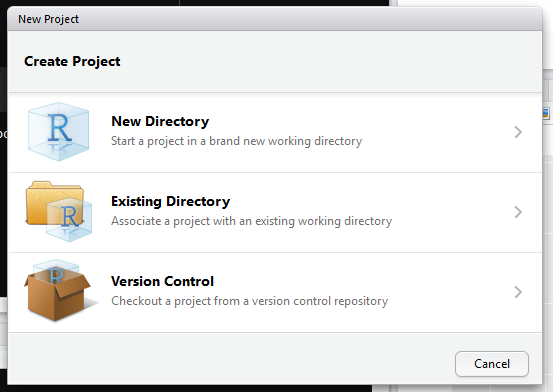
\includegraphics[width=0.8\linewidth]{img/rstudio_create_project} 

}

\caption{Creating a R project}\label{fig:r-projects}
\end{figure}

Below, we will go through the steps for creating an ``R Project'':

\begin{itemize}
\tightlist
\item
  Start R Studio (presentation of R Studio -below- should happen here)
\item
  Under the \texttt{File} menu, click on \texttt{New\ project}, choose \texttt{New\ directory}, then
  \texttt{Empty\ project}
\item
  Enter a name for this new folder (or ``directory'', in computer science), and
  choose a convenient location for it. This will be your \textbf{working directory}
  for the rest of the day (e.g., \texttt{\textasciitilde{}/bspr-workshop})
\item
  Click on ``Create project''
\item
  Under the \texttt{Files} tab on the right of the screen, click on \texttt{New\ Folder} and
  create a folder named \texttt{data} within your newly created working directory. (e.g., \texttt{\textasciitilde{}/bspr-workshopdata})
\item
  Create a new R script (File \textgreater{} New File \textgreater{} R script) and save it in your working
  directory (e.g.~\texttt{bspr-workshop-script.R})
\end{itemize}

\hypertarget{names}{%
\section{Naming things}\label{names}}

\href{https://ropensci.org/blog/2017/12/08/rprofile-jenny-bryan/}{Jenny Bryan}
has three principles for \href{http://www2.stat.duke.edu/~rcs46/lectures_2015/01-markdown-git/slides/naming-slides/naming-slides.pdf}{naming things} that are well worth remembering.

When you names something, a file or an object, ideally it should be:

\begin{enumerate}
\def\labelenumi{\arabic{enumi}.}
\tightlist
\item
  Machine readable (no whitespace, punctuation, upper AND lowercase\ldots{})
\item
  Human readable (makes sense in 6 months or 2 years time)
\item
  Plays well with default ordering (numerical or date order)
\end{enumerate}

\hypertarget{seeking-help}{%
\section{Seeking help}\label{seeking-help}}

If you need help with a specific R function, let's say \texttt{barplot()}, you can type:

\begin{Shaded}
\begin{Highlighting}[]
\NormalTok{?barplot}
\end{Highlighting}
\end{Shaded}

If you can't find what you are looking for, you can use the
\href{http://www.rdocumentation.org}{rdocumention.org} website that searches through
the help files across all packages available.

A Google or internet search ``R \textless{}task\textgreater{}'' will often either send you to the appropriate package documentation or a helpful forum question that someone else already asked,
such as \href{http://stackoverflow.com/questions/tagged/r}{Stack Overflow} or
the \href{https://community.rstudio.com/}{RStudio Community}.

\hypertarget{asking-for-help}{%
\subsection{Asking for help}\label{asking-for-help}}

As well as knowing \href{https://www.tidyverse.org/help/\#where-to-ask}{where to ask}, the key to get help
from someone is for them to grasp your problem rapidly. You
should make it as easy as possible to pinpoint where the issue might be.

Try to use the correct words to describe your problem. For instance, a
package is not the same thing as a library. Most people will understand
what you meant, but others have really strong feelings about the difference
in meaning. The key point is that it can make things confusing for people
trying to help you. Be as precise as possible when describing your problem.

If possible, try to reduce what doesn't work to a simple \emph{reproducible
example} otherwise known as a \emph{reprex}.

For more information on how to write a reproducible example see
\href{https://www.tidyverse.org/help/\#reprex}{this article}.

\hypertarget{tidyverse}{%
\chapter{Getting started in R and the tidyverse}\label{tidyverse}}

Functions are a way to automate common tasks and R comes with a set of functions
called the \texttt{base} package. We will be using some \texttt{base} functions in
Chapter \ref{transform}, but to introduce the concept of using \protect\hyperlink{function-anatomy}{functions}
we'll begin with the \texttt{tidyverse}.

\hypertarget{the-tidyverse-and-tidy-data}{%
\section{The tidyverse and tidy data}\label{the-tidyverse-and-tidy-data}}

The \href{https://www.tidyverse.org/}{tidyverse} \citep{R-tidyverse} is \emph{``an opinionated
collection of R packages designed for data science''} .

Tidyverse packages contain functions that \emph{``share an underlying design
philosophy, grammar, and data structures.''} It's this philiosophy that makes
tidyverse functions and packages relatively easy to learn and use.

Tidy data follows three principals for tabular data as proposed in the Tidy Data
paper \url{http://www.jstatsoft.org/v59/i10/paper} :

\begin{enumerate}
\def\labelenumi{\arabic{enumi}.}
\tightlist
\item
  Every variable has its own column.
\item
  Every observation has its own row.
\item
  Each value has its own cell.
\end{enumerate}

If our table was proteomics data then, we might have a set of variables such
as the peptide sequence, mass or length observed for a number of peptides.
Therefore each peptide would have a row with columns for peptide sequence, mass
and length with the value for each variable in separate cells, as
seen in Figure \ref{fig:tidy-prot}.



\begin{figure}

{\centering 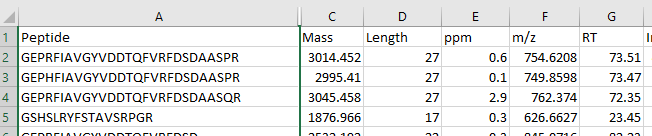
\includegraphics[width=0.8\linewidth]{img/tidy_prot_data} 

}

\caption{An example of tidy proteomics data}\label{fig:tidy-prot}
\end{figure}

Often much of the work in any data analysis is getting our data into a tidy form.

We can't do everything in the tidyverse, and everything we can do in the
tidyverse can be done in what is called base R or other packages, but the
motivation behind the tidyverse is to ease the pain of data manipulation.

With this in mind, the two tasks we are most likely to want to do
in data science are:

\begin{enumerate}
\def\labelenumi{\arabic{enumi}.}
\tightlist
\item
  Visualise our data
\item
  Automate our processes.
\end{enumerate}

Taking our cue from \href{http://r4ds.had.co.nz/}{R4DS} let's try an example.

\hypertarget{data-visualisation}{%
\section{Data visualisation}\label{data-visualisation}}

The \texttt{ggplot2} package implements the \emph{grammer of graphics}, for describing
and building graphs.

The motivation here is twofold:

\begin{enumerate}
\def\labelenumi{\arabic{enumi}.}
\tightlist
\item
  To begin to grasp the grammar of graphics approach to creating plots. This will
  be our first example of automating a task using a function.
\item
  To demonstrate how plotting is often the most useful thing we can do when
  trying to understand our data.
\end{enumerate}

We'll use the \texttt{mpg} dataset that comes with the tidyverse to examine
the question \emph{do cars with big engines use more fuel than cars with small engines?}

Try \texttt{?mpg} to learn more about the data.

\begin{enumerate}
\def\labelenumi{\arabic{enumi}.}
\tightlist
\item
  Engine size in litres is in the \texttt{displ} column.
\item
  Fuel efficiency on the highway in miles per gallon is given in the \texttt{hwy} column.
\end{enumerate}

To create a plot of engine size \texttt{displ} (x-axis) against fuel efficiency \texttt{hwy} (y-axis) we do the following:

\begin{enumerate}
\def\labelenumi{\arabic{enumi}.}
\tightlist
\item
  Use the \texttt{ggplot()} function to create an empty graph.
\item
  Provide ggplot with a first input or \textbf{argument} of the data (here \texttt{mpg}).
\item
  Then we follow the ggplot function with a \texttt{+} sign to indicate
  we are going to add more code, followed by a \texttt{geom\_point()} function to add a
  layer of points mapping some aesthetics for the x and y axes.
\item
  Mapping is always paired to aesthetics \texttt{aes()}. An aesthetic is a visual
  property of the objects in your plot, such a point size, shape or point colour.
\end{enumerate}

Therefore to plot engine size (x-axis) against fuel efficiency (y-axis) we
use the following code:

\begin{Shaded}
\begin{Highlighting}[]
\KeywordTok{ggplot}\NormalTok{(}\DataTypeTok{data =}\NormalTok{ mpg) }\OperatorTok{+}\StringTok{ }
\StringTok{  }\KeywordTok{geom_point}\NormalTok{(}\DataTypeTok{mapping =} \KeywordTok{aes}\NormalTok{(}\DataTypeTok{x =}\NormalTok{ displ, }\DataTypeTok{y =}\NormalTok{ hwy))}
\end{Highlighting}
\end{Shaded}

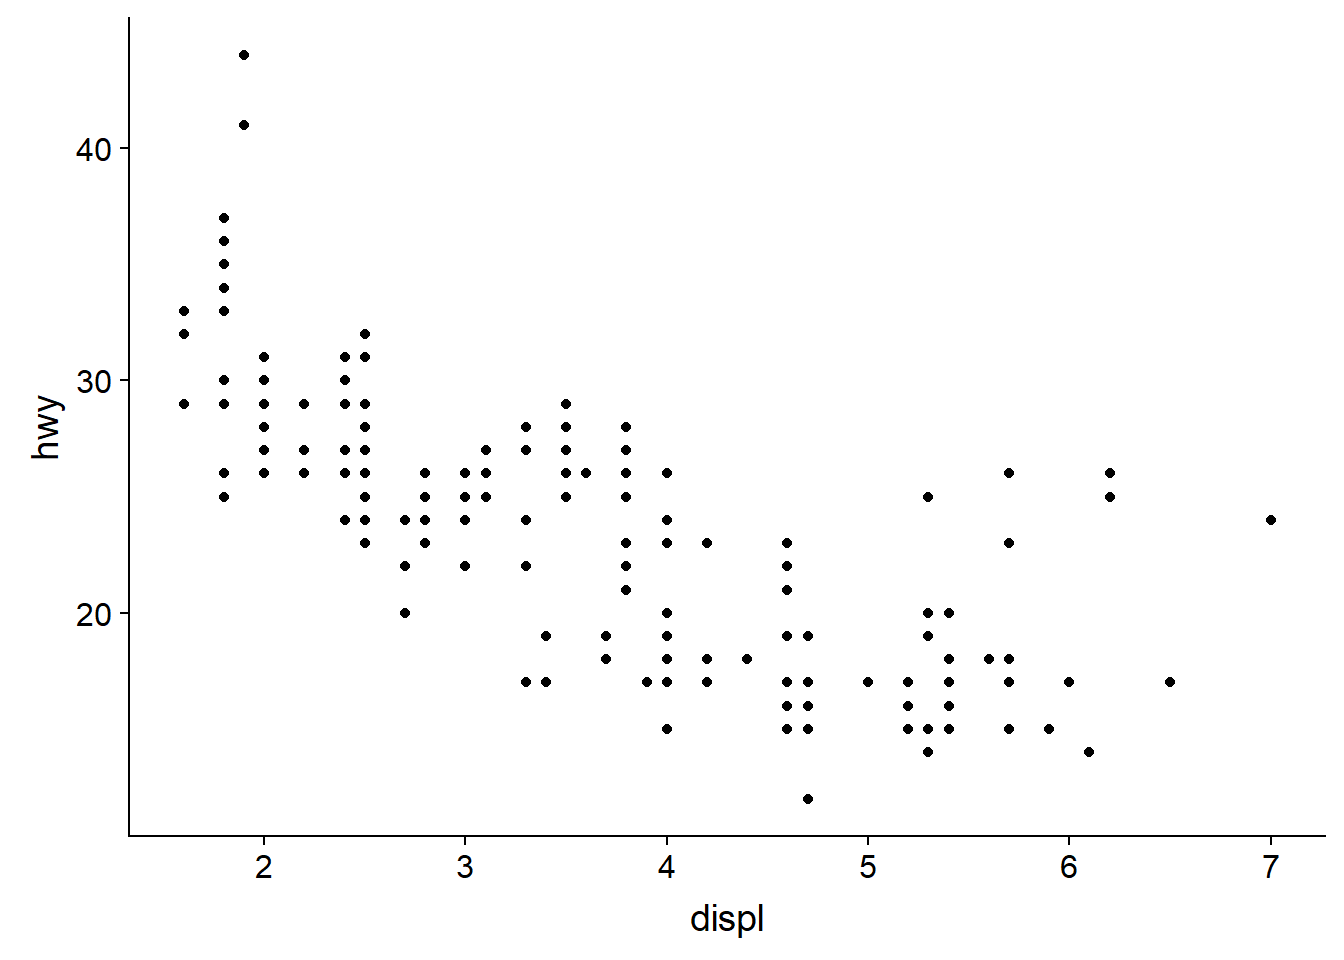
\includegraphics{bspr-workshop-2018_files/figure-latex/mpg-plot-1,mpg_point_plot-1.pdf}

This plot shows a negative relationship between engine size and fuel
efficiency.

Now try extending this code to include to add a \texttt{colour} aesthetic to the
the \texttt{aes()} function, let \texttt{colour\ =\ class}, \texttt{class} being the veichle type.
This should create a plot with as before but with the points coloured
according to the viechle type to expand our understanding.

\begin{Shaded}
\begin{Highlighting}[]
\KeywordTok{ggplot}\NormalTok{(}\DataTypeTok{data =}\NormalTok{ mpg) }\OperatorTok{+}\StringTok{ }
\StringTok{  }\KeywordTok{geom_point}\NormalTok{(}\DataTypeTok{mapping =} \KeywordTok{aes}\NormalTok{(}\DataTypeTok{x =}\NormalTok{ displ, }\DataTypeTok{y =}\NormalTok{ hwy, }\DataTypeTok{colour =}\NormalTok{ class))}
\end{Highlighting}
\end{Shaded}

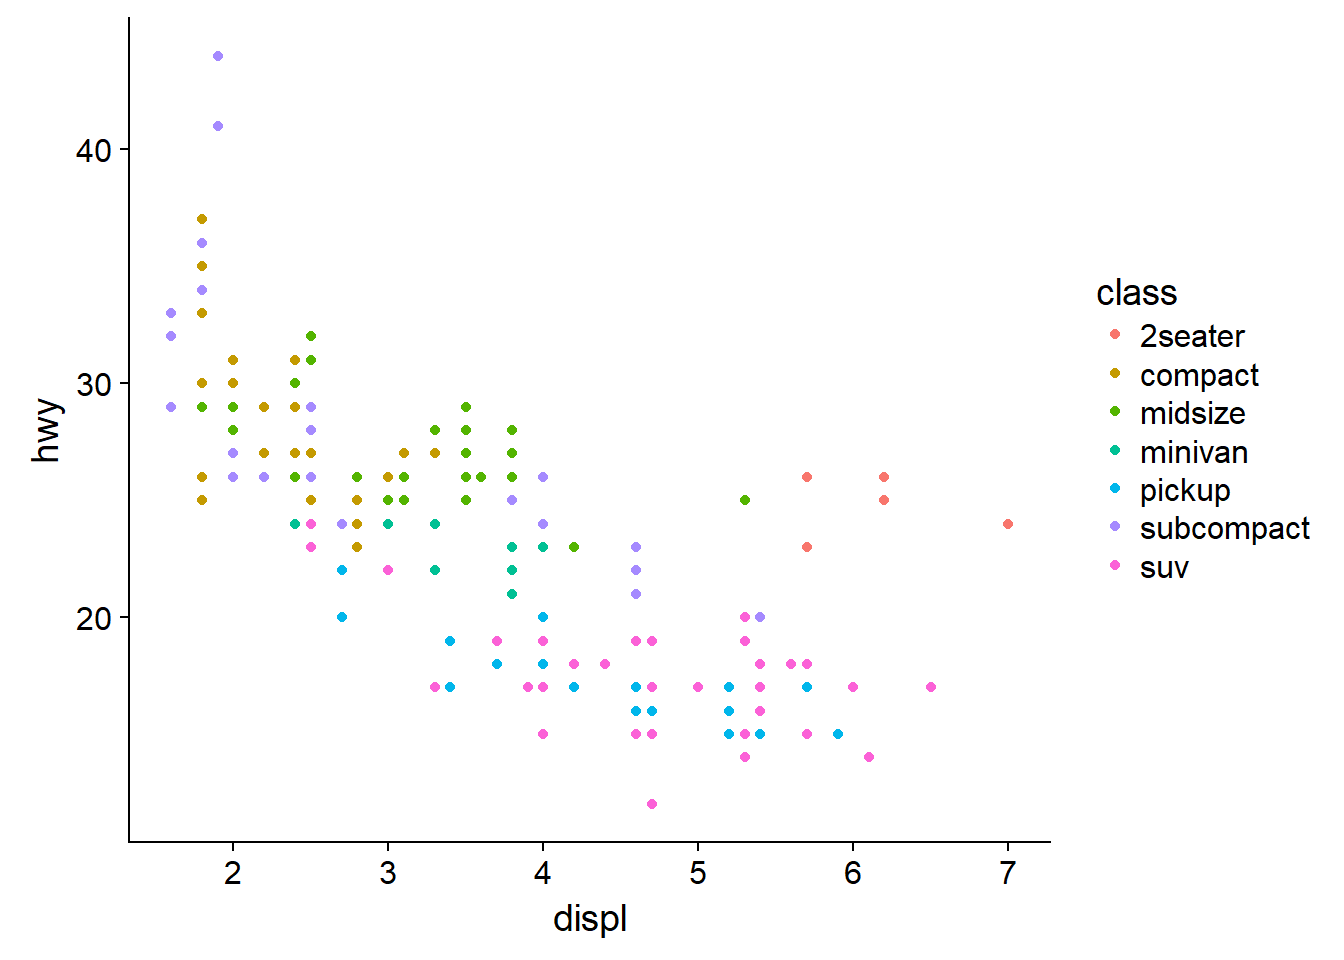
\includegraphics{bspr-workshop-2018_files/figure-latex/mpg-plot-2-1.pdf}

Now we can see that as we might expect, bigger cars such as SUVs tend to have
bigger engines and are also less fuel efficient, but some smaller cars such as
2-seaters also have big engines and greater fuel efficiency. Hence we have a
more nuanced view with this additional aesthetic.

Check out the ggplot2 documentation for all the aesthetic possibilities (and
Google for examples): \url{http://ggplot2.tidyverse.org/reference/}

So now we have re-usable code snippet for generating plots in R:

\begin{Shaded}
\begin{Highlighting}[]
\KeywordTok{ggplot}\NormalTok{(}\DataTypeTok{data =} \OperatorTok{<}\NormalTok{DATA}\OperatorTok{>}\NormalTok{) }\OperatorTok{+}\StringTok{ }
\StringTok{  }\ErrorTok{<}\NormalTok{GEOM_FUNCTION}\OperatorTok{>}\NormalTok{(}\DataTypeTok{mapping =} \KeywordTok{aes}\NormalTok{(}\OperatorTok{<}\NormalTok{MAPPINGS}\OperatorTok{>}\NormalTok{))}
\end{Highlighting}
\end{Shaded}

Concretely, in our first example \texttt{\textless{}DATA\textgreater{}} was \texttt{mpg}, the \texttt{\textless{}GEOM\_FUNCTION\textgreater{}}
was \texttt{geom\_point()} and the arguments we supplies to map our aesthetics
\texttt{\textless{}MAPPINGS\textgreater{}} were \texttt{x\ =\ displ,\ y\ =\ hwy}.

As we can use this code for any tidy data set, hopefully you are beginning to
see how a small amount of code can do a lot.

\hypertarget{viz}{%
\subsection{Visualisations}\label{viz}}

Claus Wilke has written a very nice guide to visualising data using R called
\href{http://serialmentor.com/dataviz/index.html}{Fundamentals of Data Visualization}.

\hypertarget{workflow-basics}{%
\section{Workflow basics}\label{workflow-basics}}

Let's run through the basics of working in R to conclude this chapter.

\hypertarget{assigning-objects}{%
\subsection{Assigning objects}\label{assigning-objects}}

Objects are just a way to store data inside the R environment. We create objects using the assignment operator \texttt{\textless{}-}:

\begin{Shaded}
\begin{Highlighting}[]
\NormalTok{mass_kg <-}\StringTok{ }\DecValTok{55}
\end{Highlighting}
\end{Shaded}

Read this as \emph{``mass\_kg gets value 55''} in your head.

Using \texttt{\textless{}-} can be annoying to type, so use RStudio's keyboard short cut:
Alt + - (the minus sign) to make life easier.

Many people ask why we use this assignment operator when we can use \texttt{=} instead?

\href{https://twitter.com/_colinfay/status/1006139974377443328}{Colin Fay had a Twitter thread on this subject},
but the reason I favour most is that it provides clarity. The arrow points in
the direction of the assigment (it is actually possible to assign in the other
direction too) and it distinguishes between creating an object in the workspace
and assigning a value inside a function.

Object name style is a matter of choice, but must start with a letter and can
only contain letters, numbers, \texttt{\_} and \texttt{.}. We recommend using descriptive names
and using \texttt{\_} between words. Some special symbols cannot be used in variable
names, so watch out for those.

So here we've used the name to indicate its value represents a mass in kilograms.
Look in your environment pane and you'll see the \texttt{mass\_kg} object
containing the (data) value 55.

We can inspect an object by typing it's name:

\begin{Shaded}
\begin{Highlighting}[]
\NormalTok{mass_kg}
\end{Highlighting}
\end{Shaded}

\begin{verbatim}
## [1] 55
\end{verbatim}

What's wrong here?

\begin{Shaded}
\begin{Highlighting}[]
\NormalTok{mass_KG}
\end{Highlighting}
\end{Shaded}

\texttt{Error:\ object\ \textquotesingle{}mass\_KG\textquotesingle{}\ not\ found}

This error illustrates that typos matter, everything must be precise and \texttt{mass\_KG}
is not the same as \texttt{mass\_kg}. \texttt{mass\_KG} doesn't exist, hence the error.

\hypertarget{function-anatomy}{%
\subsection{Function anatomy}\label{function-anatomy}}

Functions in R are objects followed by parentheses, such as \texttt{library()}.

Functions have the form:

\texttt{function\_name(arg1\ =\ val,\ arg2\ =\ val2,\ ...)}

The use of arguements or inputs allows us to generalise. That is to say not
just do something in a specific case, but in many cases. For example not just
make a scatter plot for the \texttt{mpg} dataset, but for any dataset of observations
that can be plotted pairwise.

Let's use \texttt{seq()} to create a \textbf{seq}uence of numbers, and at the same time practice tab completion.

Start typing \texttt{se} in the console and you should see a list of functions appear,
add \texttt{q} to shorten the list, then use the up and down arrow to highlight the function
of interest \texttt{seq()} and hit Tab to select.

RStudio puts the cursor between the parentheses to prompt us to enter some
arguments. Here we'll use 1 as the start and 10 as the end:

\begin{Shaded}
\begin{Highlighting}[]
\KeywordTok{seq}\NormalTok{(}\DecValTok{1}\NormalTok{,}\DecValTok{10}\NormalTok{)}
\end{Highlighting}
\end{Shaded}

\begin{verbatim}
##  [1]  1  2  3  4  5  6  7  8  9 10
\end{verbatim}

If we left off a parentheses to close the function, then when we hit enter
we'll see a \texttt{+} indicating RStudio is expecting further code. We either add the
missing part or press Escape to cancel the code.

Let's call a function and make an assignment at the same time. Here we'll use
the base R function \texttt{seq()} which takes three arguments: \texttt{from}, \texttt{to} and \texttt{by}.

Read the following code as \emph{"make an object called my\_sequence that stores a sequence of numbers from 2 to 20 by intervals of 2}.

\begin{Shaded}
\begin{Highlighting}[]
\NormalTok{my_sequence <-}\StringTok{ }\KeywordTok{seq}\NormalTok{(}\DecValTok{2}\NormalTok{,}\DecValTok{20}\NormalTok{,}\DecValTok{2}\NormalTok{)}
\end{Highlighting}
\end{Shaded}

This time nothing was returned to the console, but we now have an object called
\texttt{my\_sequence} in our environment.

Can you remember how to inspect it?

If we want to subset elements of \texttt{my\_sequence} we use
square brackets \texttt{{[}{]}}.

For example element five would be subset by:

\begin{Shaded}
\begin{Highlighting}[]
\NormalTok{my_sequence[}\DecValTok{5}\NormalTok{]}
\end{Highlighting}
\end{Shaded}

\begin{verbatim}
## [1] 10
\end{verbatim}

Here the number five is the index of the vector, not the value of the fifth element. The value of the fifth element is 10.

And returning multiple elements uses a colon \texttt{:}, like so

\begin{Shaded}
\begin{Highlighting}[]
\NormalTok{my_sequence[}\DecValTok{5}\OperatorTok{:}\DecValTok{8}\NormalTok{]}
\end{Highlighting}
\end{Shaded}

\begin{verbatim}
## [1] 10 12 14 16
\end{verbatim}

\hypertarget{atomics}{%
\subsection{Atomic vectors}\label{atomics}}

We actually made an atomic vector already when we made \texttt{my\_sequence}. We made a
a one dimensional group of numbers, in a sequence from two to twenty.

We're not going to be working much with atomic vectors in this workshop,
but to make you aware of how R stores data, atomic vector types
are:

\begin{itemize}
\tightlist
\item
  Doubles: regular numbers, +ve or -ve and with or without decimal places. AKA numerics.
\item
  Integers: whole numbers, specified with an upper-case L, e.g.~\texttt{int\ \textless{}-\ 2L}
\item
  Characters: Strings of text
\item
  Logicals: these store \texttt{TRUE}s and \texttt{FALSE}s which are useful for comparisons.
\item
  Complex: this would be a vector of numbers with imaginary terms.
\item
  Raw: these vectors store raw bytes of data.
\end{itemize}

Let's make a character vector and check the type:

\begin{Shaded}
\begin{Highlighting}[]
\NormalTok{cards <-}\StringTok{ }\KeywordTok{c}\NormalTok{(}\StringTok{"ace"}\NormalTok{, }\StringTok{"king"}\NormalTok{, }\StringTok{"queen"}\NormalTok{, }\StringTok{"jack"}\NormalTok{, }\StringTok{"ten"}\NormalTok{)}

\NormalTok{cards}
\end{Highlighting}
\end{Shaded}

\begin{verbatim}
## [1] "ace"   "king"  "queen" "jack"  "ten"
\end{verbatim}

\begin{Shaded}
\begin{Highlighting}[]
\KeywordTok{typeof}\NormalTok{(cards)}
\end{Highlighting}
\end{Shaded}

\begin{verbatim}
## [1] "character"
\end{verbatim}

\hypertarget{attributes}{%
\subsection{Attributes}\label{attributes}}

An attribute is a piece of information you can attach to an object, such as
names or dimensions. Attributes such as dimensions are added when
we create an object, but others such as names can be added.

Let's look at the \texttt{mpg} data frame dimensions:

\begin{Shaded}
\begin{Highlighting}[]
\CommentTok{# mpg has 234 rows (observations) and 11 columns (variables)}
\KeywordTok{dim}\NormalTok{(mpg)}
\end{Highlighting}
\end{Shaded}

\begin{verbatim}
## [1] 234  11
\end{verbatim}

\hypertarget{factors}{%
\subsection{Factors}\label{factors}}

Factors are Rs way of storing categorical information such as eye colour or
car type. A factor is something that can only have certain values, and can be
ordered (such as \texttt{low},\texttt{medium},\texttt{high}) or unordered such as types of fruit.

Factors are useful as they code string variables such as ``red'' or ``blue'' to integer values e.g.~1 and 2, which can be used in statistical models and when plotting, but they are confusing as they look like strings.

\textbf{Factors look like strings, but behave like integers.}

Historically R converts strings to factors when we load and create data, but
it's often not what we want as a default. Fortunately, in the tidyverse strings
are not treated as factors by default.

\hypertarget{lists}{%
\subsection{Lists}\label{lists}}

Lists also group data into one dimensional sets of data. The difference being
that list group objects instead of individual values, such as several atomic
vectors.

For example, let's make a list containing a vector of numbers and a character
vector

\begin{Shaded}
\begin{Highlighting}[]
\NormalTok{list_}\DecValTok{1}\NormalTok{ <-}\StringTok{ }\KeywordTok{list}\NormalTok{(}\DecValTok{1}\OperatorTok{:}\DecValTok{110}\NormalTok{,}\StringTok{"R"}\NormalTok{)}

\NormalTok{list_}\DecValTok{1}
\end{Highlighting}
\end{Shaded}

\begin{verbatim}
## [[1]]
##   [1]   1   2   3   4   5   6   7   8   9  10  11  12  13  14  15  16  17
##  [18]  18  19  20  21  22  23  24  25  26  27  28  29  30  31  32  33  34
##  [35]  35  36  37  38  39  40  41  42  43  44  45  46  47  48  49  50  51
##  [52]  52  53  54  55  56  57  58  59  60  61  62  63  64  65  66  67  68
##  [69]  69  70  71  72  73  74  75  76  77  78  79  80  81  82  83  84  85
##  [86]  86  87  88  89  90  91  92  93  94  95  96  97  98  99 100 101 102
## [103] 103 104 105 106 107 108 109 110
## 
## [[2]]
## [1] "R"
\end{verbatim}

Note the double brackets to indicate the list elements, i.e.~element one is the
vector of numbers and element two is a vector of a single character.

We won't be working with lists in this workshop, but they are a flexible way to
store data of different types in R.

Accessing list elements uses double square brackets syntax, for example
\texttt{list\_1{[}{[}1{]}{]}} would return the first vector in our list.

And to access the first element in the first vector would combine double and
single square brackets like so: \texttt{list\_1{[}{[}1{]}{]}{[}1{]}}.

Don't worry if you find this confusing, everyone does when they first start with
R.

\hypertarget{matrices-and-arrays}{%
\subsection{Matrices and arrays}\label{matrices-and-arrays}}

Matrices store values in a two dimensional array, whilst arrays can have n
dimensions. We won't be using these either, but they are also valid R objects.

\hypertarget{data-frames}{%
\subsection{Data frames}\label{data-frames}}

Data frames are two dimensional versions of lists, and this is form of storing
data we are going to be using. In a data frame each atomic vector type becomes
a column, and a data frame is formed by columns of vectors of the same length.
Each column element must be of the same type, but the column types can vary.

Figure \ref{fig:df} shows an example data frame we'll refer to as
saved as the object \texttt{df} consisting of three rows and three columns. Each
column is a different atomic data type of the same length.



\begin{figure}

{\centering 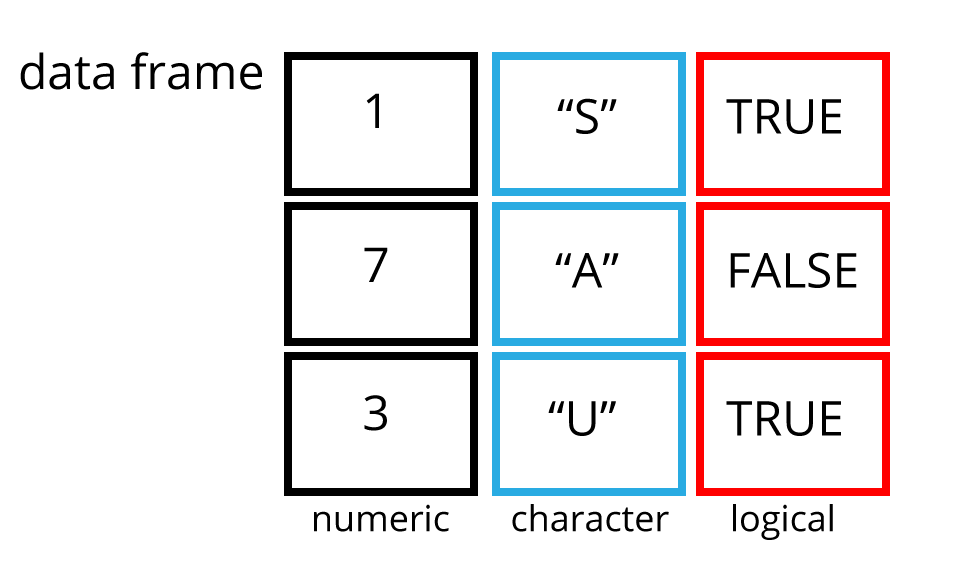
\includegraphics[width=0.8\linewidth]{img/data_frame} 

}

\caption{An example data frame \texttt{df}.}\label{fig:df}
\end{figure}

Packages in the tidyverse create a modified form of data frame called a tibble.
You can read about tibbles \href{http://r4ds.had.co.nz/tibbles.html}{here}. One
advantage of tibbles is that they don't default to treating strings as factors.
We deal with modifying data frames when we work with our example data set.

Sub-setting data frames can also be done with square bracket syntax, but as we
have both rows and columns, we need to provide index values for both row and
column.

For example \texttt{df{[}1,2{]}} means \textbf{return the value of \texttt{df} row 1, column 2}. This corresponds with the value \texttt{A}.

We can also use the colon operator to choose
several rows or columns, and by leaving the row or column blank we return all
rows or all columns.

\begin{Shaded}
\begin{Highlighting}[]
\CommentTok{# Subset rows 1 and 2 of column 1}
\NormalTok{df[}\DecValTok{1}\OperatorTok{:}\DecValTok{2}\NormalTok{,}\DecValTok{1}\NormalTok{]}

\CommentTok{# Subset all rows of column 3}
\NormalTok{df[,}\DecValTok{3}\NormalTok{]}
\end{Highlighting}
\end{Shaded}

Again don't worry too much about this for now, we won't be doing to much of this
in this lesson, but it's important to be aware of the basic syntax.

\hypertarget{learning-more-r}{%
\section{Learning more R}\label{learning-more-r}}

There are many places to start, but swirl can teach you interactively, and at your own pace in RStudio.

Just follow the instructions via this link: \url{http://swirlstats.com/students.html}

\emph{Hands-On Programming with R} by Garrett Grolemund is another great resource
for learning R.

Plus all the \href{https://www.tidyverse.org/learn/}{tidyverse links}.

\hypertarget{import}{%
\chapter{Creating scripts and importing data}\label{import}}

Our analysis is of an example data set of observations for 7702 proteins
from cells in three control experiments and three treatment experiments.
The observations are signal intensity measurements from the mass spectrometer.
These intensities relate the concentration of protein observed in each experiment
and under each condition.

We consider raw data as the data as we receive it. This doesn't mean it hasn't be
processed in some way, it just means it hasn't been processed by us.
Generally speaking we don't change the raw data file, what we do is import it and
create an object in R which we then transform.

So let's understand how to import some data.

\hypertarget{some-definitions}{%
\section{Some definitions}\label{some-definitions}}

\begin{itemize}
\tightlist
\item
  \textbf{Importing} means getting data into our R environment by creating an object
  that we can then manipulate. The raw data file remains unchanged.
\item
  \textbf{Inspecting} means looking at the dataset to understand what it contains.
\item
  \textbf{Tidying} refers to getting data into a consistent format that makes it easy
  to use in later steps.
\end{itemize}

\hypertarget{file-formats}{%
\subsection{Rectangular data and flat formats}\label{file-formats}}

Two further things to note:

\begin{enumerate}
\def\labelenumi{\arabic{enumi}.}
\item
  Here we are only considering \textbf{rectangular data}, the sort that comes
  in rows and columns such as in a spreadsheet. Lots of our data types exist,
  such as images, but can also be
  handled by R. As mentioned in \ref{biocondutor} genomic data in particular has
  led to a project called \href{http://bioconductor.org/}{Bioconductor} for the
  development of analysis tools primarily in R, many of which deal with
  non-rectangular data, but this is beyond the scope here.
\item
  \textbf{Flat formats} are files that only contain plain text, with each line
  representing a set of observations and the variables separated by delimiters
  such as tabs, commas or spaces. Therefore there aren't multiple tables such
  as we'd get in an Excel file, or meta-data such as the colour highlighting of
  a cell in an Excel file. The advantages of flat files is that they can be
  opened and used by many different computing languages or programs.
  So unless there is a good reason not to use a flat format, and there are good
  reasons, they are the best way to store data in many situations.
\end{enumerate}

\hypertarget{using-scripts}{%
\section{Using scripts}\label{using-scripts}}

Using the console is useful, but as we build up a workflow, that is to say,
writing code to:

\begin{itemize}
\tightlist
\item
  load packages
\item
  load data
\item
  explore the data
\item
  and output some results
\end{itemize}

Then it's much more useful to contain this in a script: a document of our code.

Why? When we write and save our code in scripts, we can re-use it, share it or
edit it. But \textbf{most importantly a script is a record}.

Cmd/Ctrl + Shift + N will open a new script file up and you should see something
like Figure \ref{fig:script-pane} with the script editor pane open:



\begin{figure}

{\centering 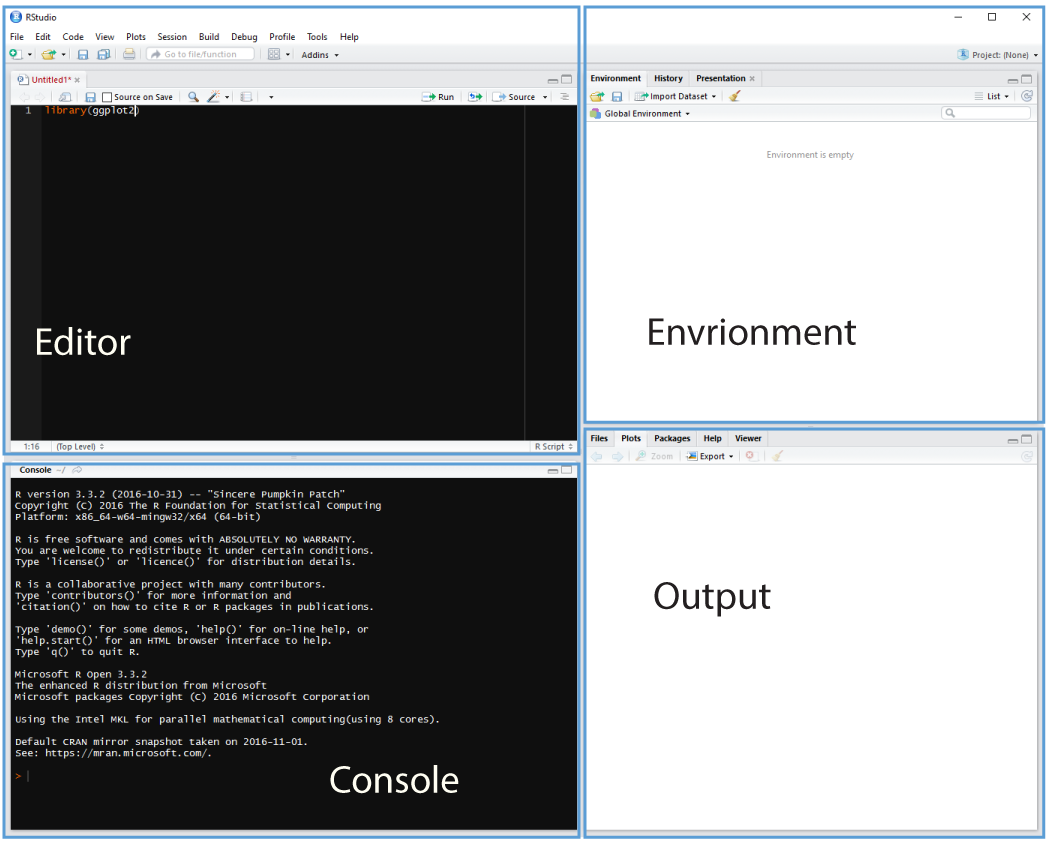
\includegraphics[width=0.8\linewidth]{img/rstudio_screenshot_four_panes} 

}

\caption{Rstudio with the script editor pane open.}\label{fig:script-pane}
\end{figure}

\hypertarget{running-code}{%
\section{Running code}\label{running-code}}

We can run a highlighted portion of code in your script if you click the Run
button at the top of the scripts pane as shown in Figure \ref{fig:run-script}.



\begin{figure}

{\centering 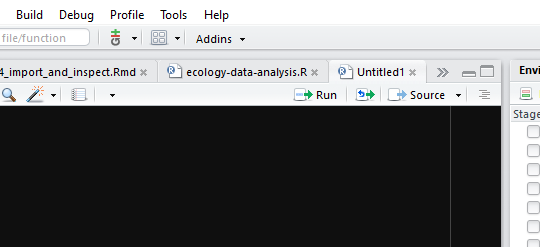
\includegraphics[width=0.8\linewidth]{img/run_script} 

}

\caption{Scripts can be run by clicking the Source button.}\label{fig:run-script}
\end{figure}

You can run the entire script by clicking the Source button.

Or we can run chunks of code if we split our script into sections, see below.

\hypertarget{creating-a-r-script}{%
\section{Creating a R script}\label{creating-a-r-script}}

We first need to create a script that will form the basis of our analysis.

Go to the file menu and select New Files \textgreater{} R script. This should open the script
editor pane.

Now let's save the script, by going to File \textgreater{} Save and we should find ourselves
prompted to save the script in our Project Directory.

Following the advice about \protect\hyperlink{names}{naming things} we can create a new R script
called \texttt{01-bspr-workshop-july-2018}.

This name is machine readable (no spaces or special characters), human readable,
and works well with default ordering by beginning with \texttt{01}.

\hypertarget{setting-up-our-environment}{%
\section{Setting up our environment}\label{setting-up-our-environment}}

At the head of our script it's common to put a title, the name of the author
and the date, and any other useful information. This is created as comments
using the \texttt{\#} at the start of each line.

It's then usual to follow this by code to load the packages we need into our
our R environment using the \texttt{library()} function and providing the name of the
package we wish to load. Packages are collections of R functions.

Often we break the code up into regions by adding dashes (or equals symbols)
to the comment line. This enables us to run chunks of the script separately from
running the whole script when using our code.

Here is a typical head for a script:

\begin{Shaded}
\begin{Highlighting}[]
\CommentTok{# My workshop script}
\CommentTok{# 7th July 2018}
\CommentTok{# Alistair Bailey}

\CommentTok{# Load packages ----------------------------------------------------------------}
\KeywordTok{library}\NormalTok{(plyr)}
\KeywordTok{library}\NormalTok{(tidyverse)}
\KeywordTok{library}\NormalTok{(gplots)}
\KeywordTok{library}\NormalTok{(pheatmap)}
\KeywordTok{library}\NormalTok{(gridExtra)}
\KeywordTok{library}\NormalTok{(VennDiagram)}
\KeywordTok{library}\NormalTok{(ggseqlogo)}
\end{Highlighting}
\end{Shaded}

\hypertarget{biocondutor}{%
\subsection{Bioconductor}\label{biocondutor}}

As an aside there are many proteomics specific R packages, these are generally
found through \href{https://www.bioconductor.org/}{Bioconductor} which is a project
that was initiated in 2001 to create tools for the analysis of high-throughput
genomic data, but also includes other 'omics data tools \citep[\citet{huber2015}]{gentleman2004}.

Exploring Bioconductor is beyond our scope here, but well worth exploring for
manipulation and analysis of raw data formats such as mzxml files.

\hypertarget{importing-data}{%
\section{Importing data}\label{importing-data}}

Assuming our data is in a \protect\hyperlink{file-formats}{flat format}, we can import it into our
environment using the tidyverse \texttt{readr} package.

If our data was an excel file, we can use the tidyverse \texttt{readxl} package to
import the data, but it will remove any meta-data and each table in the excel
file will become a separate R object as per tidy data principles.

For the purposes of this workshop we have a \texttt{csv} (comma separated variable) file.

If you haven't done so already
Click here to download the example data and save it to our project
directory. Check the \texttt{Files} pane to see it's there.

We then import data and assign it to an object we'll call \texttt{data} like so:

\begin{Shaded}
\begin{Highlighting}[]
\CommentTok{# Import example data ----------------------------------------------------------}
\CommentTok{# Import the example data with read_csv from the readr package}
\NormalTok{dat <-}\StringTok{ }\NormalTok{readr}\OperatorTok{::}\KeywordTok{read_csv}\NormalTok{(}\StringTok{"data/070718-proteomics-example-data.csv"}\NormalTok{)}
\end{Highlighting}
\end{Shaded}

\begin{verbatim}
## Parsed with column specification:
## cols(
##   protein_accession = col_character(),
##   protein_description = col_character(),
##   control_1 = col_double(),
##   control_2 = col_double(),
##   control_3 = col_double(),
##   treatment_1 = col_double(),
##   treatment_2 = col_double(),
##   treatment_3 = col_double()
## )
\end{verbatim}

\hypertarget{exploring-the-data}{%
\section{Exploring the data}\label{exploring-the-data}}

\hypertarget{glimpse-head-and-str}{%
\subsection{\texorpdfstring{\texttt{glimpse}, \texttt{head} and \texttt{str}}{glimpse, head and str}}\label{glimpse-head-and-str}}

The first thing to do with any data set is to actually look at it. Here are
four ways to have look at the data in the \texttt{Console}: calling the object directly,
\texttt{glimpse}, \texttt{head} and \texttt{str}.

\begin{enumerate}
\def\labelenumi{\arabic{enumi}.}
\tightlist
\item
  We can just call the object and return it to the \texttt{Console}, which may or may
  not be useful depending on the size and type of object we call.
\end{enumerate}

2 .\texttt{glimpse} is a tidyverse function that tries to show us as much data in
a data.frame or tibble as possible, telling us the \protect\hyperlink{atomics}{atomic types} of
data in the table, the number of observations and the number of variables, and
importantly shows all the column variable names by transposing the table.

\begin{enumerate}
\def\labelenumi{\arabic{enumi}.}
\setcounter{enumi}{2}
\item
  \texttt{head} is a base function that shows us the 6 lines of a R object by default.
\item
  \texttt{str} is a base function that show the structure of a R object, so it provides
  a lot of information, but is not so easy to read.
\end{enumerate}

The outputs for these four functions is shown below:

\begin{Shaded}
\begin{Highlighting}[]
\CommentTok{# call object}
\NormalTok{dat}
\end{Highlighting}
\end{Shaded}

\begin{verbatim}
## # A tibble: 7,702 x 8
##    protein_accessi~ protein_descrip~ control_1 control_2 control_3
##    <chr>            <chr>                <dbl>     <dbl>     <dbl>
##  1 VATA_HUMAN_P386~ V-type proton A~     0.811     0.858     1.04 
##  2 RL35A_HUMAN_P18~ 60S ribosomal p~     0.367     0.385     0.409
##  3 MYH10_HUMAN_P35~ Myosin-10 OS=Ho~     2.98      4.62      2.87 
##  4 RHOG_HUMAN_P840~ Rho-related GTP~     0.142     0.224     0.128
##  5 PSA1_HUMAN_P257~ Proteasome subu~     1.07      0.945     0.803
##  6 PRDX5_HUMAN_P30~ Peroxiredoxin-5~     0.566     0.540     0.488
##  7 ACLY_HUMAN_P533~ ATP-citrate syn~     5.00      4.22      5.03 
##  8 VDAC2_HUMAN_P45~ Voltage-depende~     1.35      1.33      1.14 
##  9 LRC47_HUMAN_Q8N~ Leucine-rich re~     0.927     0.770     1.17 
## 10 CH60_HUMAN_P108~ 60 kDa heat sho~     9.45      8.41     10.4  
## # ... with 7,692 more rows, and 3 more variables: treatment_1 <dbl>,
## #   treatment_2 <dbl>, treatment_3 <dbl>
\end{verbatim}

\begin{Shaded}
\begin{Highlighting}[]
\CommentTok{# tidyverse glimpse function}
\KeywordTok{glimpse}\NormalTok{(dat)}
\end{Highlighting}
\end{Shaded}

\begin{verbatim}
## Observations: 7,702
## Variables: 8
## $ protein_accession   <chr> "VATA_HUMAN_P38606", "RL35A_HUMAN_P18077",...
## $ protein_description <chr> "V-type proton ATPase catalytic subunit A ...
## $ control_1           <dbl> 0.8114, 0.3672, 2.9815, 0.1424, 1.0748, 0....
## $ control_2           <dbl> 0.8575, 0.3853, 4.6176, 0.2238, 0.9451, 0....
## $ control_3           <dbl> 1.0381, 0.4091, 2.8709, 0.1281, 0.8032, 0....
## $ treatment_1         <dbl> 0.6448, 0.4109, 7.1670, 0.1643, 0.7884, 0....
## $ treatment_2         <dbl> 0.7190, 0.4634, 2.0052, 0.2466, 0.8798, 1....
## $ treatment_3         <dbl> 0.4805, 0.3561, 0.8995, 0.1268, 0.7631, 0....
\end{verbatim}

\begin{Shaded}
\begin{Highlighting}[]
\CommentTok{# head function}
\KeywordTok{head}\NormalTok{(dat)}
\end{Highlighting}
\end{Shaded}

\begin{verbatim}
## # A tibble: 6 x 8
##   protein_accessi~ protein_descrip~ control_1 control_2 control_3
##   <chr>            <chr>                <dbl>     <dbl>     <dbl>
## 1 VATA_HUMAN_P386~ V-type proton A~     0.811     0.858     1.04 
## 2 RL35A_HUMAN_P18~ 60S ribosomal p~     0.367     0.385     0.409
## 3 MYH10_HUMAN_P35~ Myosin-10 OS=Ho~     2.98      4.62      2.87 
## 4 RHOG_HUMAN_P840~ Rho-related GTP~     0.142     0.224     0.128
## 5 PSA1_HUMAN_P257~ Proteasome subu~     1.07      0.945     0.803
## 6 PRDX5_HUMAN_P30~ Peroxiredoxin-5~     0.566     0.540     0.488
## # ... with 3 more variables: treatment_1 <dbl>, treatment_2 <dbl>,
## #   treatment_3 <dbl>
\end{verbatim}

\begin{Shaded}
\begin{Highlighting}[]
\CommentTok{# str function}
\KeywordTok{str}\NormalTok{(dat)}
\end{Highlighting}
\end{Shaded}

\begin{verbatim}
## Classes 'spec_tbl_df', 'tbl_df', 'tbl' and 'data.frame': 7702 obs. of  8 variables:
##  $ protein_accession  : chr  "VATA_HUMAN_P38606" "RL35A_HUMAN_P18077" "MYH10_HUMAN_P35580" "RHOG_HUMAN_P84095" ...
##  $ protein_description: chr  "V-type proton ATPase catalytic subunit A OS=Homo sapiens GN=ATP6V1A PE=1 SV=2" "60S ribosomal protein L35a OS=Homo sapiens GN=RPL35A PE=1 SV=2" "Myosin-10 OS=Homo sapiens GN=MYH10 PE=1 SV=3" "Rho-related GTP-binding protein RhoG OS=Homo sapiens GN=RHOG PE=1 SV=1" ...
##  $ control_1          : num  0.811 0.367 2.982 0.142 1.075 ...
##  $ control_2          : num  0.858 0.385 4.618 0.224 0.945 ...
##  $ control_3          : num  1.038 0.409 2.871 0.128 0.803 ...
##  $ treatment_1        : num  0.645 0.411 7.167 0.164 0.788 ...
##  $ treatment_2        : num  0.719 0.463 2.005 0.247 0.88 ...
##  $ treatment_3        : num  0.48 0.356 0.899 0.127 0.763 ...
##  - attr(*, "spec")=
##   .. cols(
##   ..   protein_accession = col_character(),
##   ..   protein_description = col_character(),
##   ..   control_1 = col_double(),
##   ..   control_2 = col_double(),
##   ..   control_3 = col_double(),
##   ..   treatment_1 = col_double(),
##   ..   treatment_2 = col_double(),
##   ..   treatment_3 = col_double()
##   .. )
\end{verbatim}

To see the data in a \emph{spreadsheet} fashion use \texttt{View(dat)}, note the capital V
and a new tab will open. This can also be launched from the \texttt{Environment} tab by
clicking on \texttt{dat}.

Although this provides us with some useful information, such as the number of
observations and variables, to understand more plotting the data will be
helpful as we'll see in Section \ref{normalisation}.

\hypertarget{summary-statisitics}{%
\subsection{Summary statisitics}\label{summary-statisitics}}

Another useful way to quickly get a sense of the data is to use the \texttt{summary}
function, which will return summary of the spread of the data and importantly
if there are missing values. We can see immediately below that the experimental
replicates have different distributions, and missing values that we need to
deal with in Chapter \ref{transform}.

\begin{Shaded}
\begin{Highlighting}[]
\KeywordTok{summary}\NormalTok{(dat)}
\end{Highlighting}
\end{Shaded}

\begin{verbatim}
##  protein_accession  protein_description   control_1        control_2     
##  Length:7702        Length:7702         Min.   : 0.001   Min.   : 0.000  
##  Class :character   Class :character    1st Qu.: 0.143   1st Qu.: 0.132  
##  Mode  :character   Mode  :character    Median : 0.345   Median : 0.322  
##                                         Mean   : 0.933   Mean   : 0.845  
##                                         3rd Qu.: 0.959   3rd Qu.: 0.845  
##                                         Max.   :31.944   Max.   :31.697  
##                                         NA's   :4888     NA's   :4828    
##    control_3       treatment_1      treatment_2      treatment_3    
##  Min.   : 0.001   Min.   : 0.000   Min.   : 0.002   Min.   : 0.002  
##  1st Qu.: 0.149   1st Qu.: 0.112   1st Qu.: 0.135   1st Qu.: 0.101  
##  Median : 0.388   Median : 0.286   Median : 0.319   Median : 0.254  
##  Mean   : 0.977   Mean   : 0.795   Mean   : 0.856   Mean   : 0.675  
##  3rd Qu.: 0.999   3rd Qu.: 0.780   3rd Qu.: 0.880   3rd Qu.: 0.682  
##  Max.   :31.320   Max.   :41.686   Max.   :28.234   Max.   :21.428  
##  NA's   :5087     NA's   :4739     NA's   :4902     NA's   :5074
\end{verbatim}

\hypertarget{dplyr}{%
\chapter{\texorpdfstring{\texttt{dplyr} verbs and piping}{dplyr verbs and piping}}\label{dplyr}}

A core package in the tidyverse is \texttt{dplyr} for transforming data, which is often
used in conjunction with the \texttt{magrittr} package that allows us to pipe multiple
operations together.

The R4DS dplyr chapter is \href{http://r4ds.had.co.nz/transform.html}{here} and for
magrittr \href{http://r4ds.had.co.nz/pipes.html}{here}.

The figures in this chapter we made for use with an ecological dataset on rodent
surveys, but the principles they illustrate are generic and show the use of
each function with or without the use of a pipe.

From R4DS:

"\emph{All \texttt{dplyr} verbs work similarly:}

\emph{1. The first argument is a data frame.}

\emph{2. The subsequent arguments describe what to do with the data frame, using the variable names (without quotes).}

\emph{3. The result is a new data frame.}

\emph{Together these properties make it easy to chain together multiple simple steps to achieve a complex result.}"

\hypertarget{pipes}{%
\section{Pipes}\label{pipes}}

A pipe in R looks like this \texttt{\%\textgreater{}\%} and allows us to send the output of one
operation into another. This saves time and space, and can make our code easier
to read.

For example we can pipe the output of calling the \texttt{dat} object into the \texttt{glimpse}
function like so:

\begin{Shaded}
\begin{Highlighting}[]
\NormalTok{dat }\OperatorTok\StringTok{ }\KeywordTok{glimpse}\NormalTok{()}
\end{Highlighting}
\end{Shaded}

\begin{verbatim}
## Observations: 7,702
## Variables: 8
## $ protein_accession   <chr> "VATA_HUMAN_P38606", "RL35A_HUMAN_P18077",...
## $ protein_description <chr> "V-type proton ATPase catalytic subunit A ...
## $ control_1           <dbl> 0.8114, 0.3672, 2.9815, 0.1424, 1.0748, 0....
## $ control_2           <dbl> 0.8575, 0.3853, 4.6176, 0.2238, 0.9451, 0....
## $ control_3           <dbl> 1.0381, 0.4091, 2.8709, 0.1281, 0.8032, 0....
## $ treatment_1         <dbl> 0.6448, 0.4109, 7.1670, 0.1643, 0.7884, 0....
## $ treatment_2         <dbl> 0.7190, 0.4634, 2.0052, 0.2466, 0.8798, 1....
## $ treatment_3         <dbl> 0.4805, 0.3561, 0.8995, 0.1268, 0.7631, 0....
\end{verbatim}

This becomes even more useful when we combine pipes with \texttt{dplyr} functions.

\hypertarget{filter}{%
\section{Filter rows}\label{filter}}

The \texttt{filter} function enables us to filter the rows of a data frame according to
a logical test (one that is \texttt{TRUE} or \texttt{FALSE}). Here it filters rows in
the surveys data where the year variable is greater or equal to 1985.

\begin{center}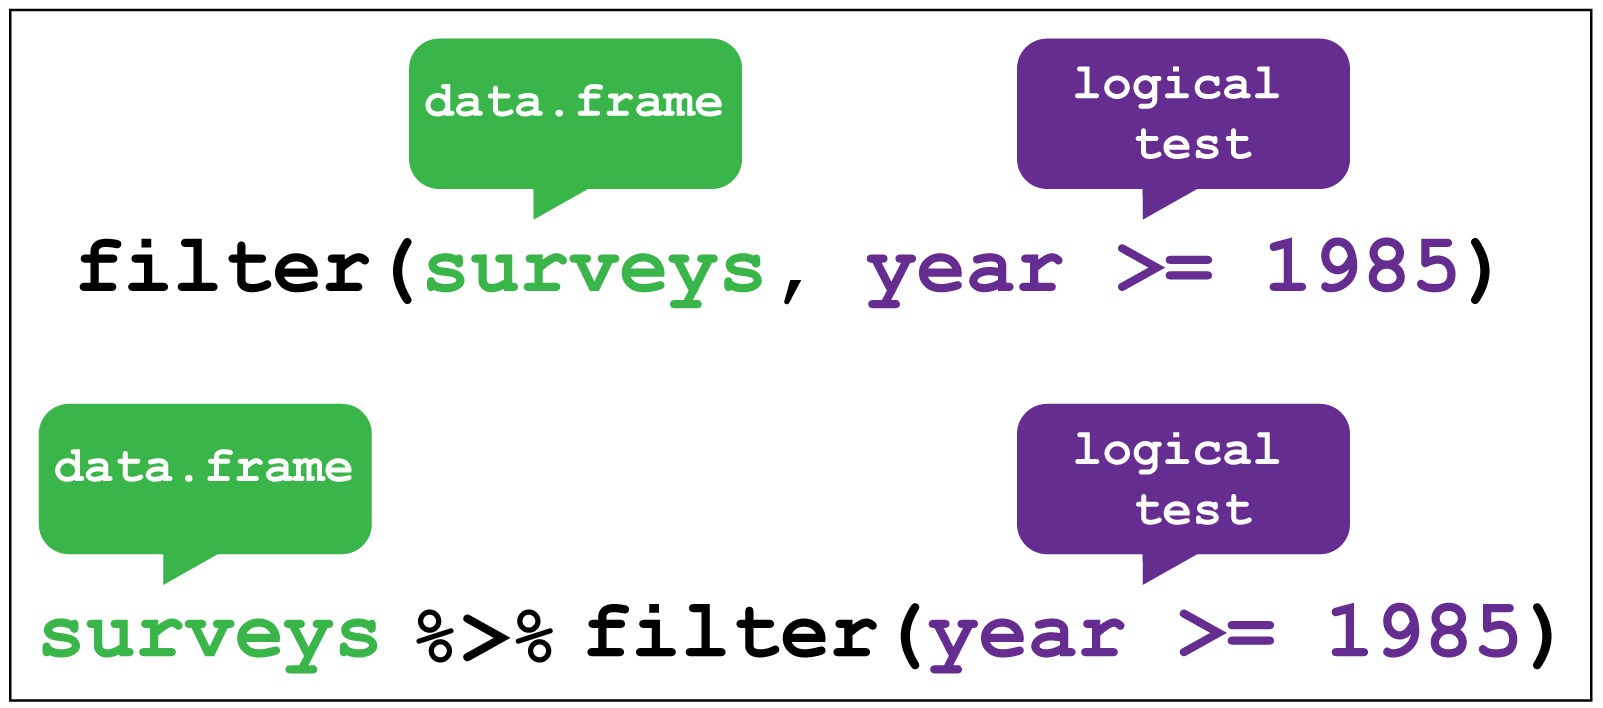
\includegraphics[width=0.8\linewidth]{img/dplyr_filter} \end{center}

Let's try this with \texttt{dat} to filter the rows for proteins in \texttt{control\_1} and
\texttt{control\_2} experiments where the observations are greater than 20:

\begin{Shaded}
\begin{Highlighting}[]
\NormalTok{dat }\OperatorTok\StringTok{ }\KeywordTok{filter}\NormalTok{(control_}\DecValTok{1} \OperatorTok{>}\StringTok{ }\DecValTok{20}\NormalTok{, control_}\DecValTok{2} \OperatorTok{>}\StringTok{ }\DecValTok{20}\NormalTok{)}
\end{Highlighting}
\end{Shaded}

\begin{verbatim}
## # A tibble: 2 x 8
##   protein_accessi~ protein_descrip~ control_1 control_2 control_3
##   <chr>            <chr>                <dbl>     <dbl>     <dbl>
## 1 MYH9_HUMAN_P355~ Myosin-9 OS=Hom~      29.2      31.7      24.6
## 2 A0A087WWY3_HUMA~ Filamin-A OS=Ho~      31.9      27.8      31.3
## # ... with 3 more variables: treatment_1 <dbl>, treatment_2 <dbl>,
## #   treatment_3 <dbl>
\end{verbatim}

Filtering is done with the following operators \texttt{\textgreater{}},\texttt{\textless{}},\texttt{\textgreater{}=},\texttt{\textless{}=},\texttt{!=} (not equal)
and \texttt{==} for equal. Not the double equal sign.

\hypertarget{arrange-rows}{%
\section{Arrange rows}\label{arrange-rows}}

Arranging is similar to filter except that it changes the row order according
to the columns in ascending order. If you provide more than one column name,
each additional column will be used to break ties in the values of preceding
columns.

Here we arrange the surveys data according to the record identification number.

\begin{center}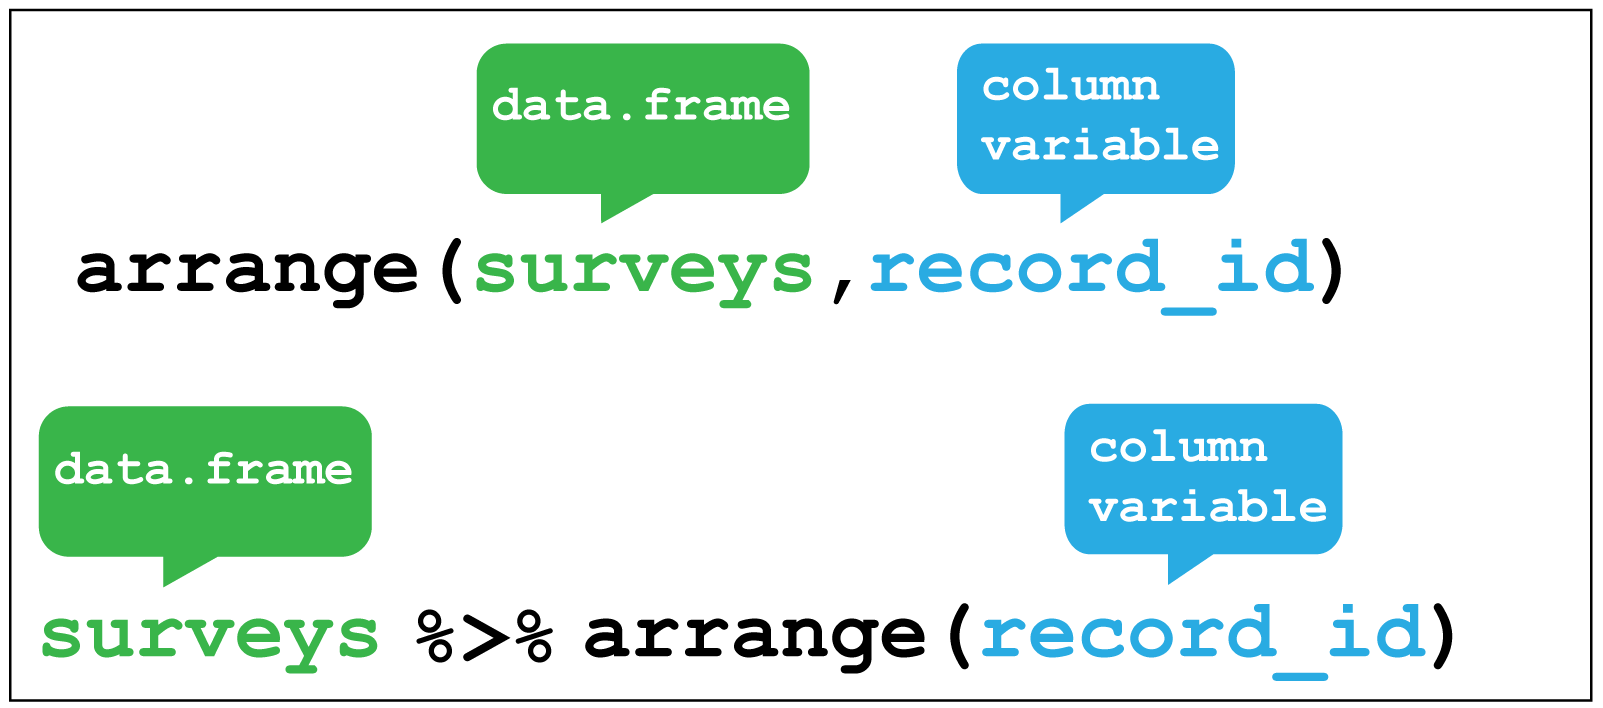
\includegraphics[width=0.8\linewidth]{img/dplyr_arrange} \end{center}

To try that with \texttt{dat} let's arrange the data according to \texttt{control\_1}:

\begin{Shaded}
\begin{Highlighting}[]
\NormalTok{dat }\OperatorTok\StringTok{ }\KeywordTok{arrange}\NormalTok{(control_}\DecValTok{1}\NormalTok{)}
\end{Highlighting}
\end{Shaded}

\begin{verbatim}
## # A tibble: 7,702 x 8
##    protein_accessi~ protein_descrip~ control_1 control_2 control_3
##    <chr>            <chr>                <dbl>     <dbl>     <dbl>
##  1 PAL4G_HUMAN_P0D~ Peptidyl-prolyl~   0.001      0.0177    NA    
##  2 E5RGV5_HUMAN_E5~ Nucleolysin TIA~   0.0011    NA          0.093
##  3 E5RJP4_HUMAN_E5~ Glutamine--fruc~   0.002     NA         NA    
##  4 I3L3U1_HUMAN_I3~ Myosin light ch~   0.00240   NA         NA    
##  5 ENPLL_HUMAN_Q58~ Putative endopl~   0.0026    NA         NA    
##  6 K1C15_HUMAN_P19~ Keratin_ type I~   0.00290    0.0615     0.122
##  7 B5ME44_HUMAN_B5~ Outer dense fib~   0.00290   NA         NA    
##  8 PANK3_HUMAN_Q9H~ Pantothenate ki~   0.0033    NA         NA    
##  9 RRS1_HUMAN_Q150~ Ribosome biogen~   0.0035    NA         NA    
## 10 NFL_HUMAN_P07196 Neurofilament l~   0.0035     0.315      0.564
## # ... with 7,692 more rows, and 3 more variables: treatment_1 <dbl>,
## #   treatment_2 <dbl>, treatment_3 <dbl>
\end{verbatim}

\hypertarget{select-columns}{%
\section{Select columns}\label{select-columns}}

Selecting is the verb we use to select columns of interest in the data. Here
we select only the \texttt{year} and \texttt{plot\_type} columns and discard the rest.

\begin{center}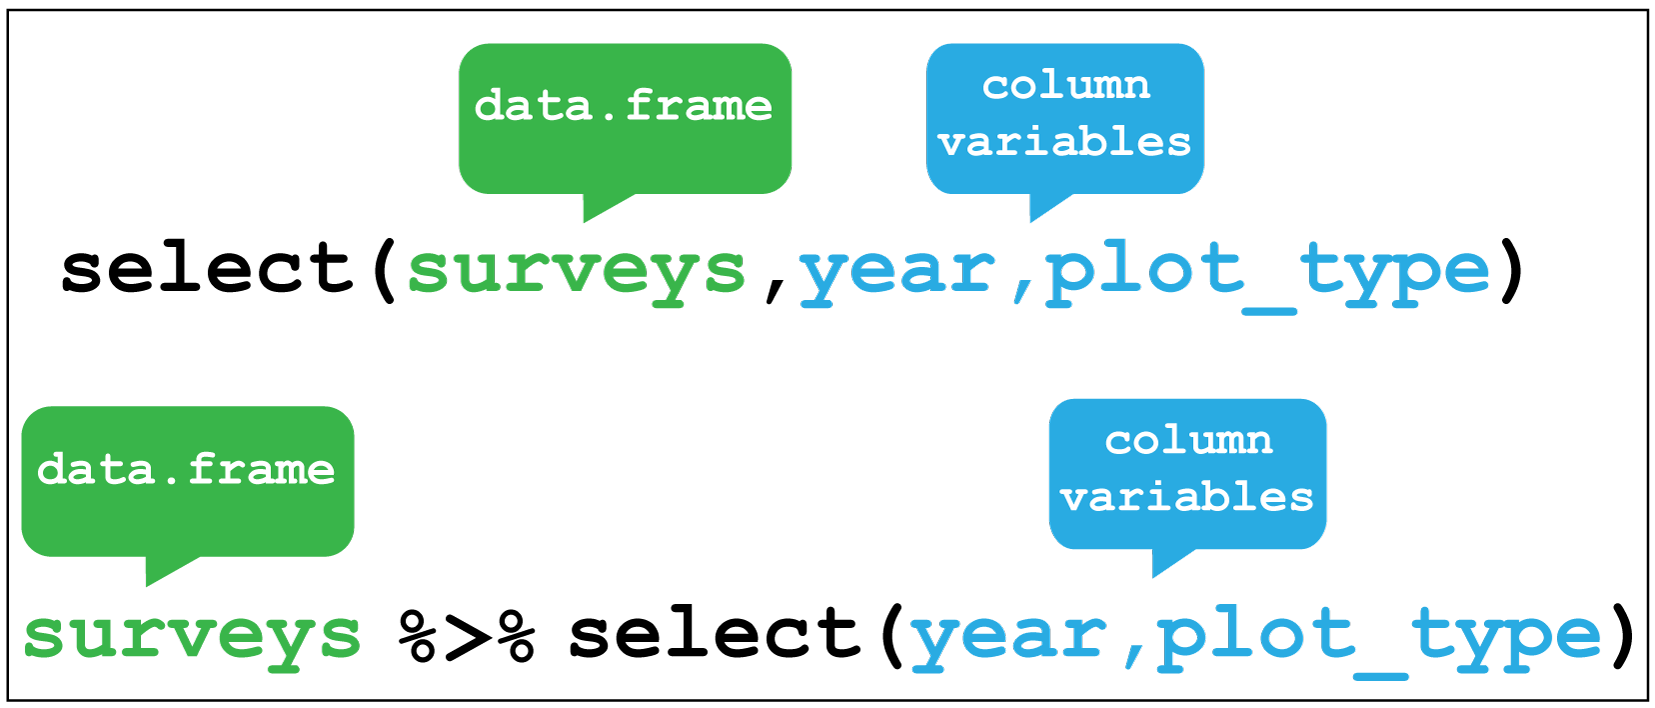
\includegraphics[width=0.8\linewidth]{img/dplyr_select} \end{center}

Let's use select with \texttt{dat} to drop the protein description and control
experiments using negative indexing and keep everything else:

\begin{Shaded}
\begin{Highlighting}[]
\NormalTok{dat }\OperatorTok\StringTok{ }\KeywordTok{select}\NormalTok{(}\OperatorTok{-}\NormalTok{protein_description,}\OperatorTok{-}\NormalTok{(control_}\DecValTok{1}\OperatorTok{:}\NormalTok{control_}\DecValTok{3}\NormalTok{))}
\end{Highlighting}
\end{Shaded}

\begin{verbatim}
## # A tibble: 7,702 x 4
##    protein_accession  treatment_1 treatment_2 treatment_3
##    <chr>                    <dbl>       <dbl>       <dbl>
##  1 VATA_HUMAN_P38606        0.645       0.719       0.480
##  2 RL35A_HUMAN_P18077       0.411       0.463       0.356
##  3 MYH10_HUMAN_P35580       7.17        2.01        0.900
##  4 RHOG_HUMAN_P84095        0.164       0.247       0.127
##  5 PSA1_HUMAN_P25786        0.788       0.880       0.763
##  6 PRDX5_HUMAN_P30044       0.545       1.69        0.821
##  7 ACLY_HUMAN_P53396        4.67        5.01        3.57 
##  8 VDAC2_HUMAN_P45880       1.01        1.04        0.904
##  9 LRC47_HUMAN_Q8N1G4       1.22        1.01        0.593
## 10 CH60_HUMAN_P10809        8.31        8.31        5.73 
## # ... with 7,692 more rows
\end{verbatim}

\hypertarget{mutate}{%
\section{Create new variables}\label{mutate}}

Creating new variables uses the \texttt{mutate} verb. Here I am creating a new
variable called \texttt{rodent\_type} that will create a new column containing the type
of rodent observed in each row.

\begin{center}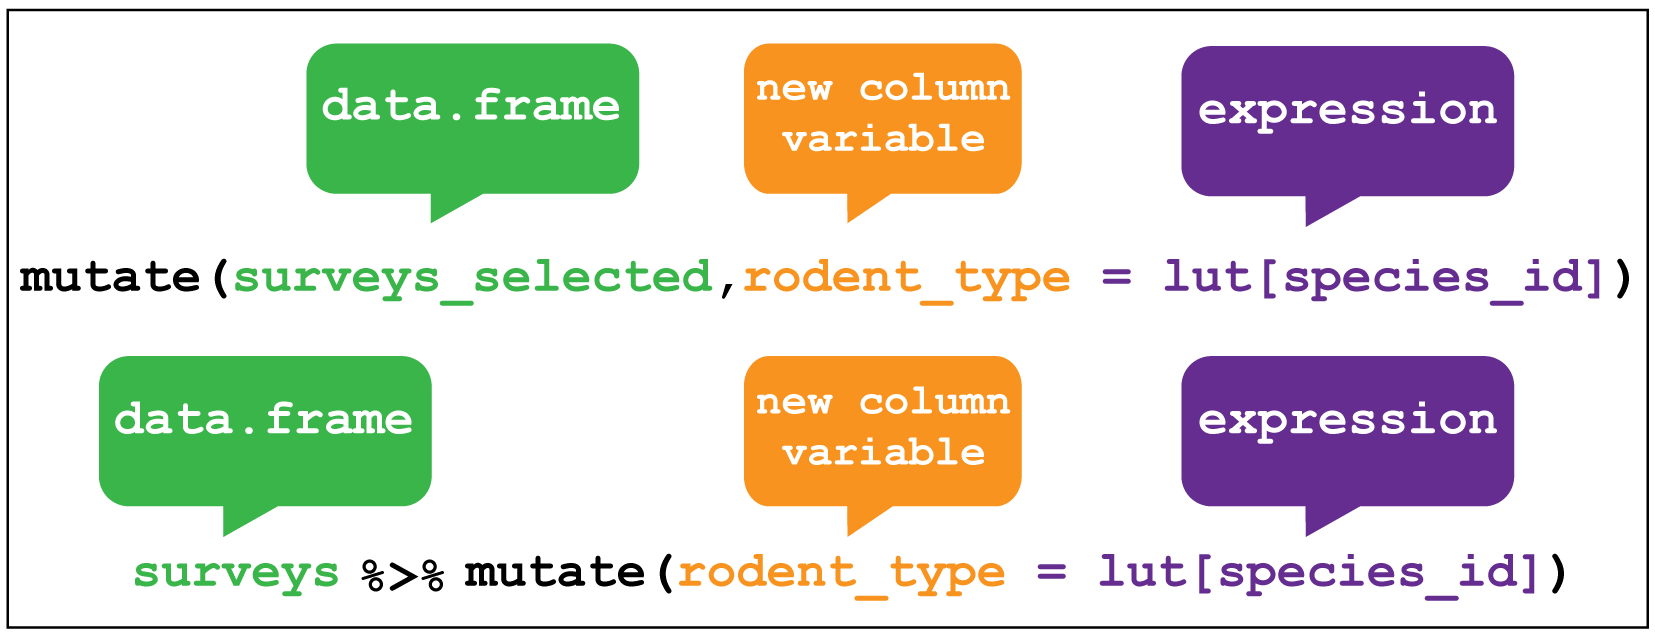
\includegraphics[width=0.8\linewidth]{img/dplyr_mutate} \end{center}

Let's create a new variable for \texttt{dat} called \texttt{prot\_id} that use the \texttt{str\_extract}
function from the \texttt{stringr} package to take the last 6 characters of
the \texttt{protein\_accession} variable, the \texttt{".\{6\}\$"} part is called a regular
expression, to keep just the UNIPROT id part of the string.

We'll use select to drop the other variables except the
protein accession afterwards via another pipe.

\begin{Shaded}
\begin{Highlighting}[]
\NormalTok{dat }\OperatorTok\StringTok{ }
\StringTok{  }\KeywordTok{mutate}\NormalTok{(}\DataTypeTok{prot_id =} \KeywordTok{str_extract}\NormalTok{(protein_accession,}\StringTok{".\{6\}$"}\NormalTok{)) }\OperatorTok\StringTok{ }
\StringTok{  }\KeywordTok{select}\NormalTok{(protein_accession, prot_id)}
\end{Highlighting}
\end{Shaded}

\begin{verbatim}
## # A tibble: 7,702 x 2
##    protein_accession  prot_id
##    <chr>              <chr>  
##  1 VATA_HUMAN_P38606  P38606 
##  2 RL35A_HUMAN_P18077 P18077 
##  3 MYH10_HUMAN_P35580 P35580 
##  4 RHOG_HUMAN_P84095  P84095 
##  5 PSA1_HUMAN_P25786  P25786 
##  6 PRDX5_HUMAN_P30044 P30044 
##  7 ACLY_HUMAN_P53396  P53396 
##  8 VDAC2_HUMAN_P45880 P45880 
##  9 LRC47_HUMAN_Q8N1G4 Q8N1G4 
## 10 CH60_HUMAN_P10809  P10809 
## # ... with 7,692 more rows
\end{verbatim}

\hypertarget{create-grouped-summaries}{%
\section{Create grouped summaries}\label{create-grouped-summaries}}

The last key verb is \texttt{summarise} which collapses a data frame
into a single row.

For example, we could use it to find the average weight
of all the animals surveyed in the surveys data using \texttt{mean()}.
(Here the \texttt{na.rm\ =\ TRUE} argument is given to remove missing values from the
data, otherwise R would return \texttt{NA} when trying to average.)

\begin{center}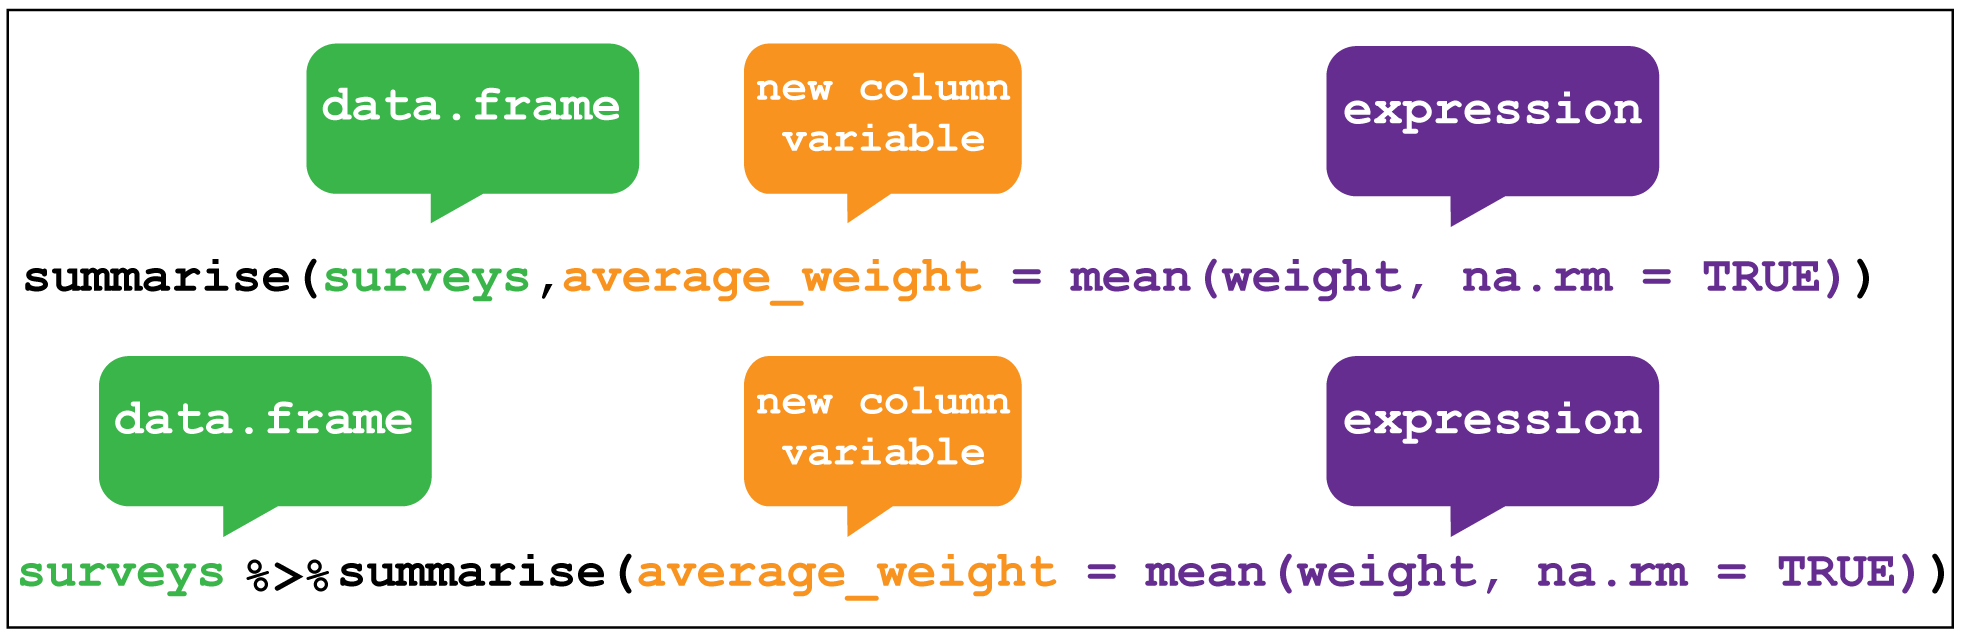
\includegraphics[width=0.8\linewidth]{img/dplyr_summarise} \end{center}

\texttt{summarise} is most useful when paired with \texttt{group\_by}
which defines the variables upon which we operate upon.

Here if we group by \texttt{species\_id} and \texttt{rodent\_type} together and then used
\texttt{summarise} without any arguments we return these two variables only.

\begin{center}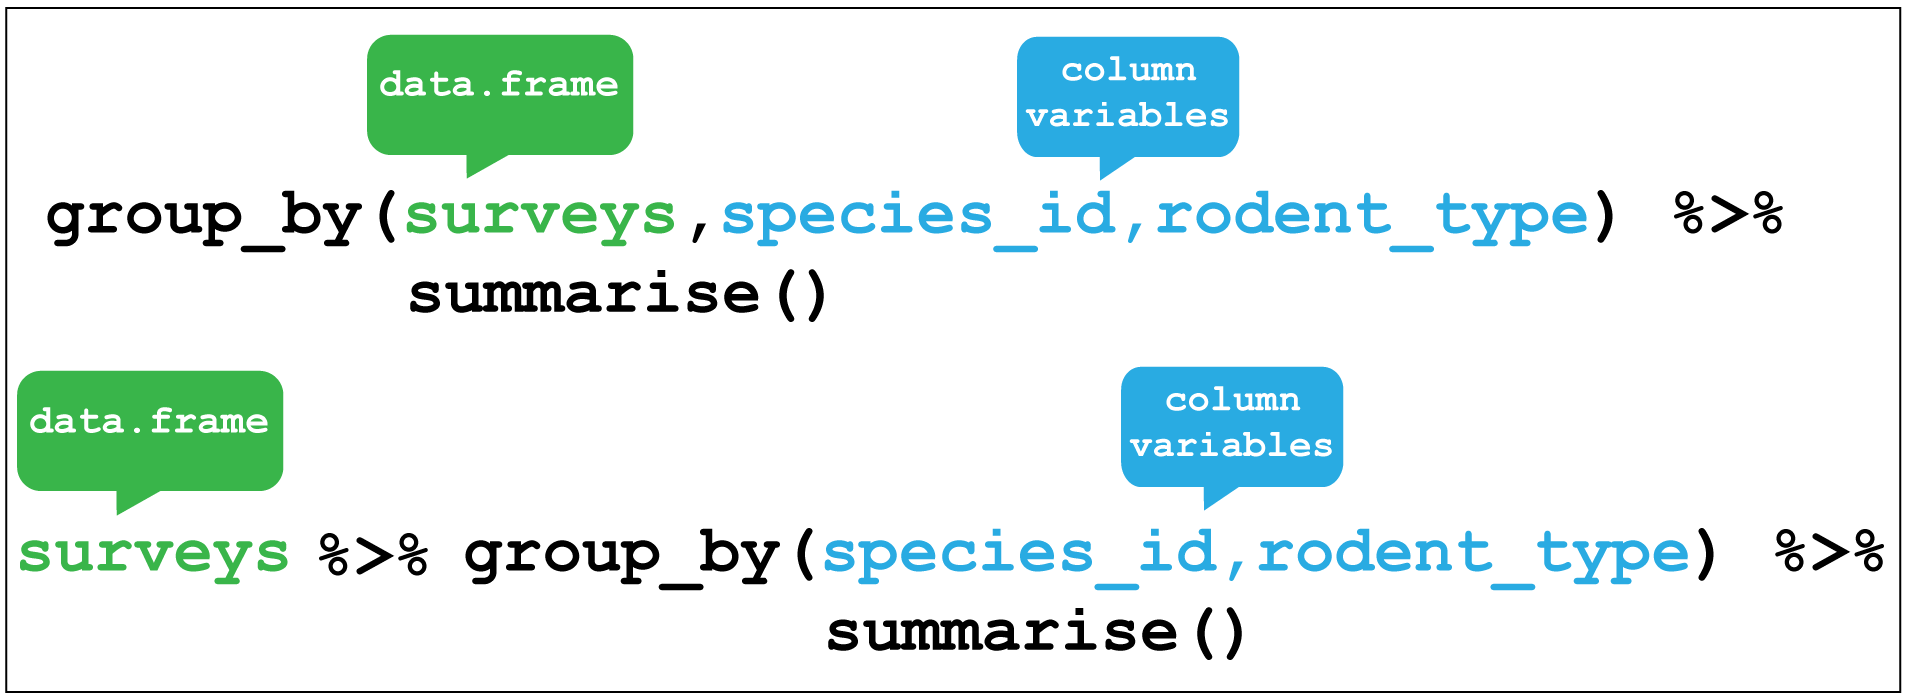
\includegraphics[width=0.8\linewidth]{img/dplyr_group_by} \end{center}

We'll use the \texttt{mpg} dataset again to illustrate a grouped summary. Here
I'll group according fuel type \texttt{fl}, c = compressed natural gas ,d = diesel,
e = ethanol, p = premium and r = regular.
Then using summarise to calculate the mean highway (\texttt{hwy}) miles per gallon,
and the mean urban (\texttt{cty}) miles per gallon,the tables is collapsed from 234 to
five rows, one for each fuel type and two columns for the mean mpg;s. This
illustrates how grouped summaries provide a very concise way of exploring data
as we can immediately see the relative fuel efficiences of each fuel type under
two conditions.

\begin{Shaded}
\begin{Highlighting}[]
\CommentTok{# fl is fuel type. c = compressed natural gas ,d = diesel, }
\CommentTok{# e = ethanol, p = premium and r = regular.}
\NormalTok{mpg }\OperatorTok\StringTok{ }
\StringTok{  }\KeywordTok{group_by}\NormalTok{(fl) }\OperatorTok\StringTok{ }
\StringTok{  }\CommentTok{# Create summaries mean_hwy and mean_cty using the mean function, }
\StringTok{  }\CommentTok{# dropping any missing variables.}
\StringTok{  }\KeywordTok{summarise}\NormalTok{(}\DataTypeTok{mean_hwy =} \KeywordTok{mean}\NormalTok{(hwy, }\DataTypeTok{na.rm =}\NormalTok{ T), }\DataTypeTok{mean_cty =} \KeywordTok{mean}\NormalTok{(cty, }\DataTypeTok{na.rm =}\NormalTok{ T))}
\end{Highlighting}
\end{Shaded}

\begin{verbatim}
## # A tibble: 5 x 3
##   fl    mean_hwy mean_cty
##   <chr>    <dbl>    <dbl>
## 1 c         36      24   
## 2 d         33.6    25.6 
## 3 e         13.2     9.75
## 4 p         25.2    17.4 
## 5 r         23.0    16.7
\end{verbatim}

We'll use \texttt{dplyr} and pipes in Chapter \ref{transform}.

\hypertarget{transform}{%
\chapter{Transforming and visualising proteomics data}\label{transform}}

Having imported our data set of observations for 7702 proteins
from cells in three control experiments and three treatment experiments.
Remember, the observations are signal intensity measurements from the mass
spectrometer, and these intensities relate to the amount of protein in each
experiment and under each condition.

Now we will transform the data to examine the effect of
the treatment on the cellular proteome and visualise the output using a volcano
plot and a heatmap. The hypothesis we are testing is that treatment
changes the concentration of protein we observe.

A volcano plot is commonly used way of plotting changes in observed values
on the x-axis against the likelihood of observing that change due to chance
on the y-axis. Heatmaps are another way of visualising the relative
(increase and decrease of) amounts of observed values.

\hypertarget{fold-change-and-log-fold-change}{%
\section{Fold change and log-fold change}\label{fold-change-and-log-fold-change}}

Fold changes are ratios, the ratio of say protein expression before and
after treatment, where a value larger than 1 for a protein implies that
protein expression was greater after the treatment.

In life sciences, fold change is often reported as log-fold change. Why is that?
There are at least two reasons which can be shown by plotting.

One is that ratios are not symmetrical around 1, so it's difficult to observe
both changes in the forwards and backwards direcion i.e.~proteins where expression
went up and proteins where expression went down due to treatment. When we
transform ratios on a log scale, the scale becomes symmetric around 0 and thus
we can now observe the distribution of ratios in terms of positive, negative or
no change.



\begin{figure}
\centering
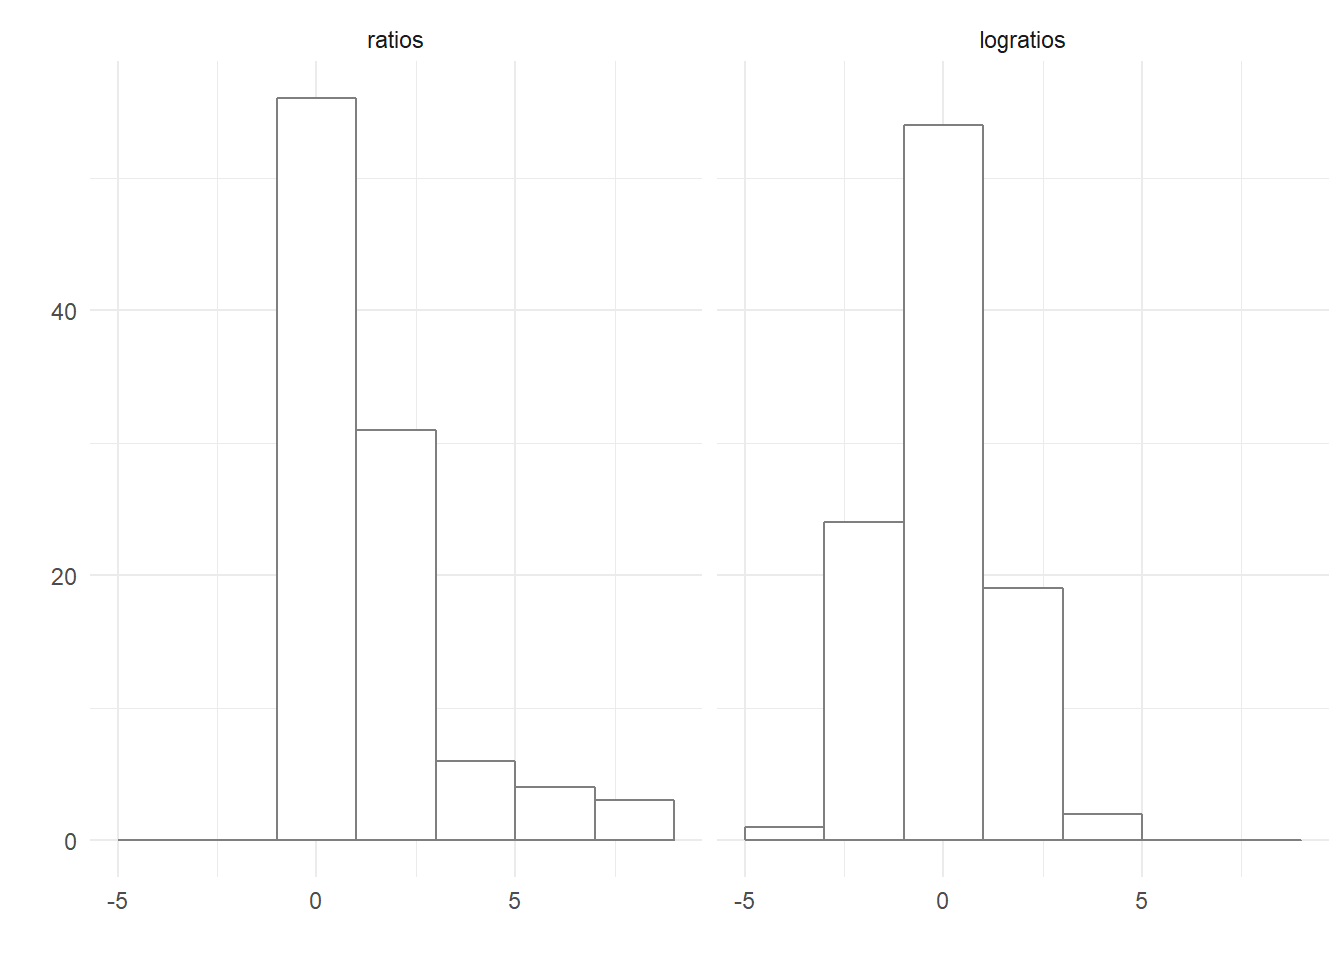
\includegraphics{bspr-workshop-2018_files/figure-latex/fold-change-1-1.pdf}
\caption{\label{fig:fold-change-1}Ratios are not symmetric around one, logratios are symmetric around zero.}
\end{figure}

A second reason is that transforming values onto a log scale changes where
the numbers actually occur when plotted on that scale. If we consider the log
scale to represent magnitudes, then we can more easily see changes of small and
large magnitudes when we plot the data.

For example, a fold change of 32 times can be either a ratio 1/32 or 32/1.

As shown in Figure \ref{fig:fold-change-2}, 1/32 is much closer to 1 than 32/1,
but transformed to a log scale we see that in terms of magnitude of difference it
is the same as 32/1.

Often the log transformation is to a base of 2 as each increment of 1 represents
a doubling, but sometimes a base of 10 is used, for example for p-values.



\begin{figure}
\centering
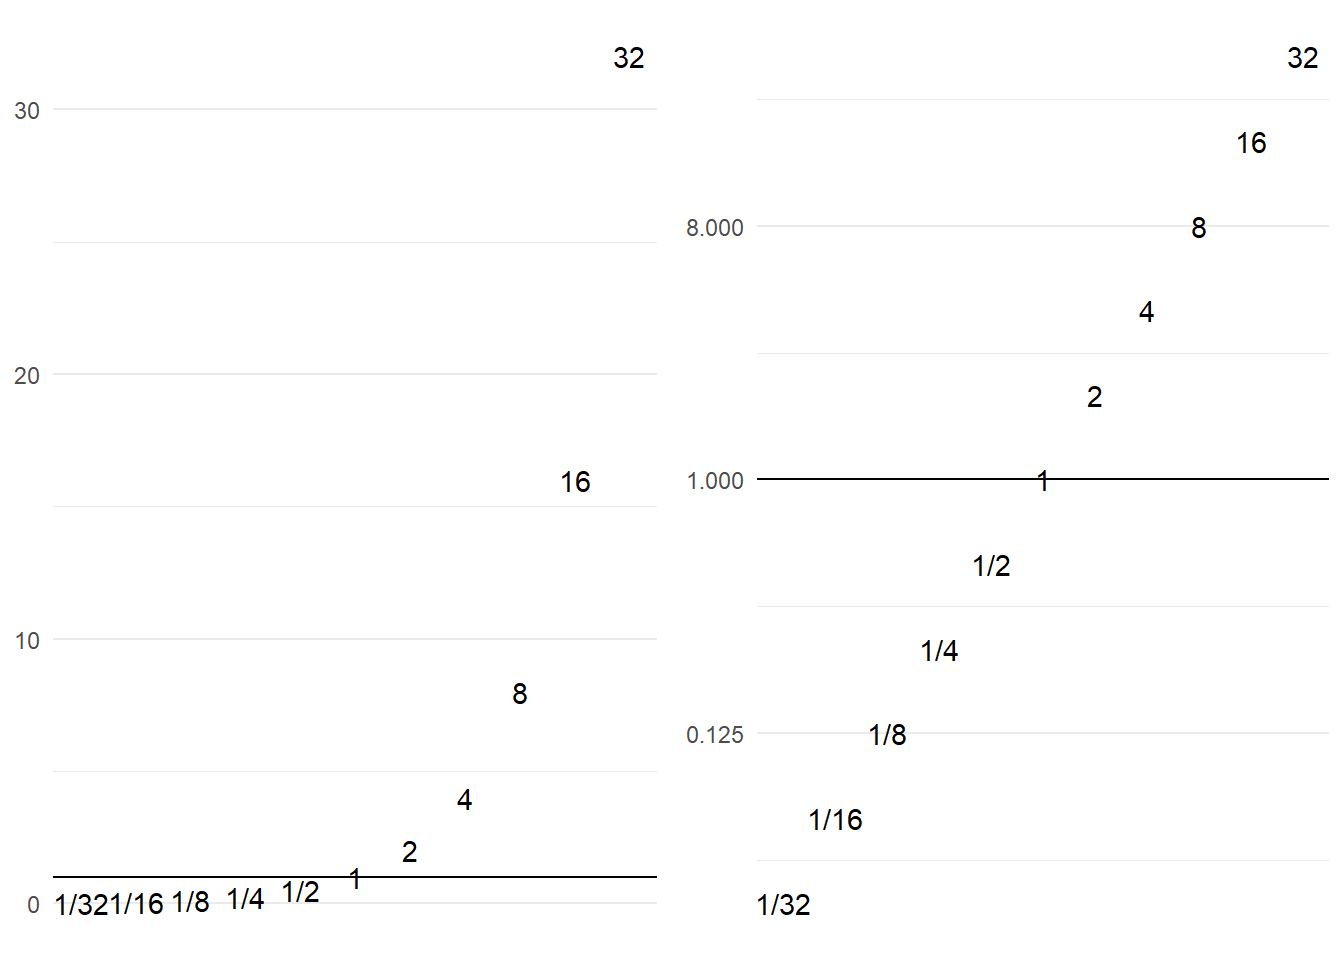
\includegraphics{bspr-workshop-2018_files/figure-latex/fold-change-2-1.pdf}
\caption{\label{fig:fold-change-2}Transformation of scales using log transformation.}
\end{figure}

\hypertarget{missing-values}{%
\section{Dealing with missing values}\label{missing-values}}

Unless we're really lucky, it's unlikely that we'll get observations for
the same numbers of proteins in all replicated experiments. This means
there will be missing values for some proteins when looking at all the
experiments together. This then raises the question of what to do about the
missing values? We have two choices:

\begin{enumerate}
\def\labelenumi{\arabic{enumi}.}
\tightlist
\item
  Only analyse the proteins that we have observations for in all experiments.
\item
  Impute values for the missing values from the existing observations.
\end{enumerate}

There are pros and cons to either approach. Here for simplicity we'll use only
the proteins for which we have observations in all assays.

We can drop the proteins with missing values by piping our data set to the
\texttt{drop\_na()} function from the \texttt{tidyr} package like so. We assign this to a new
object called \texttt{dat\_tidy}.

We'll use the summarise function to compare the number of proteins before and
after dropping the missing values using the \texttt{n()} counting function.

\begin{Shaded}
\begin{Highlighting}[]
\CommentTok{# Remove the missing values}
\NormalTok{dat_tidy <-}\StringTok{ }\NormalTok{dat }\OperatorTok\StringTok{ }\KeywordTok{drop_na}\NormalTok{()}
\CommentTok{# Nunber of proteins in original data}
\NormalTok{dat }\OperatorTok\StringTok{ }\KeywordTok{summarise}\NormalTok{(}\DataTypeTok{Number_of_proteins =} \KeywordTok{n}\NormalTok{())}
\end{Highlighting}
\end{Shaded}

\begin{verbatim}
## # A tibble: 1 x 1
##   Number_of_proteins
##                <int>
## 1               7702
\end{verbatim}

\begin{Shaded}
\begin{Highlighting}[]
\CommentTok{# Nunber of proteins without missing values}
\NormalTok{dat_tidy }\OperatorTok\StringTok{ }\KeywordTok{summarise}\NormalTok{(}\DataTypeTok{Number_of_proteins =} \KeywordTok{n}\NormalTok{())}
\end{Highlighting}
\end{Shaded}

\begin{verbatim}
## # A tibble: 1 x 1
##   Number_of_proteins
##                <int>
## 1               1145
\end{verbatim}

This shrinks the dataset from 7,702 proteins to 1,145 proteins, so we can see
why imputing the missing values might be more atrractive.

One approach you might like to try is to impute the data by replacing the
missing values with the mean observation for each protein under each condition.

\hypertarget{normalisation}{%
\section{Data normalization}\label{normalisation}}

To perform statistical inference, for example whether treatment increases or
decreases protein abundance, we need to account for the variation that occurs
from run to run on our spectrometers and each give rise to a different
distribution. This is as opposed to variation arising from treatment versus
control which we are interested in understanding. Hence normalisation seeks to
reduce the run-to-run sources of variation.

A method of normalization introduced for DNA microarray analysis is
quantile normalisation \citep{bolstad2003}. There are various ways to normalise data,
so using quantile normalisation here is primarily to demonstate the approach in
R, you should consider what is best for your data.

If we consider our proteomics data as a distribution of values, one value for
the concentration of each protein in our experiment that together form a
distribution. Figure \ref{fig:data-dist} shows the distribution of
protein concentrations observed for the three control and three treatment assays.
As we can see the distributions are different for each assay.



\begin{figure}

{\centering 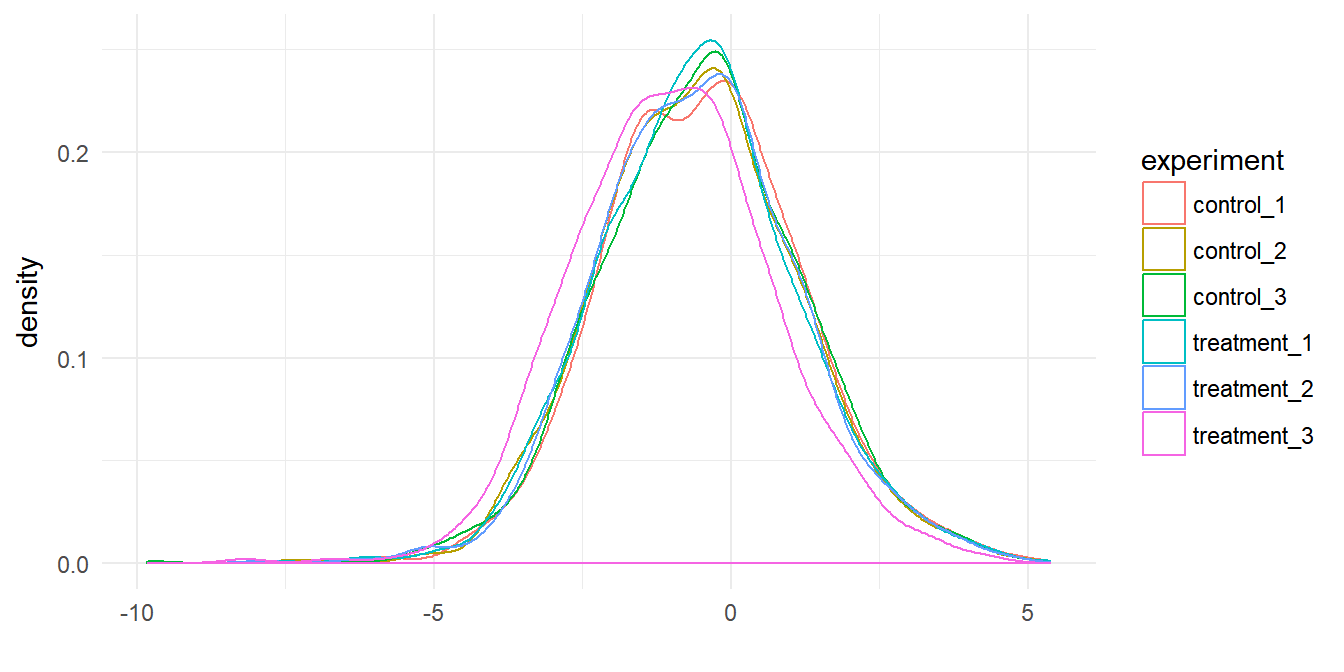
\includegraphics[width=0.8\linewidth]{bspr-workshop-2018_files/figure-latex/data-dist-1} 

}

\caption{Protein data for six assays plotted as a distributions.}\label{fig:data-dist}
\end{figure}

A quantile represents a region of distribution, for example the 0.95 quantile
is the value such that 95\% of the data lies below it. To normalize two or more
distributions with each other without recourse to a reference distribution we:

\begin{enumerate}
\def\labelenumi{(\roman{enumi})}
\tightlist
\item
  Rank the value in each experiment (represented in the columns) from
  lowest to highest. In other words identify the quantiles for each protein
  in each experiment.
\item
  Sort each experiment (the columns) from lowest to highest value.
\item
  Calculate the mean across the rows for the sorted values.
\item
  Then substitute these mean values back according to rank for each experiment
  to restore the original order.
\end{enumerate}

This results in the highest ranking observation in each experiment
becoming the mean of the highest observations across all experiments, the
second ranking observation in each experiment becoming the mean of the
second highest observations across all experiments. Therefore the
distributions for each each experiment are now the same.

\href{https://davetang.org/muse/2014/07/07/quantile-normalisation-in-r/}{Dave Tang's Blog:Quantile Normalisation in R} has more
details on this approach.



\begin{figure}

{\centering 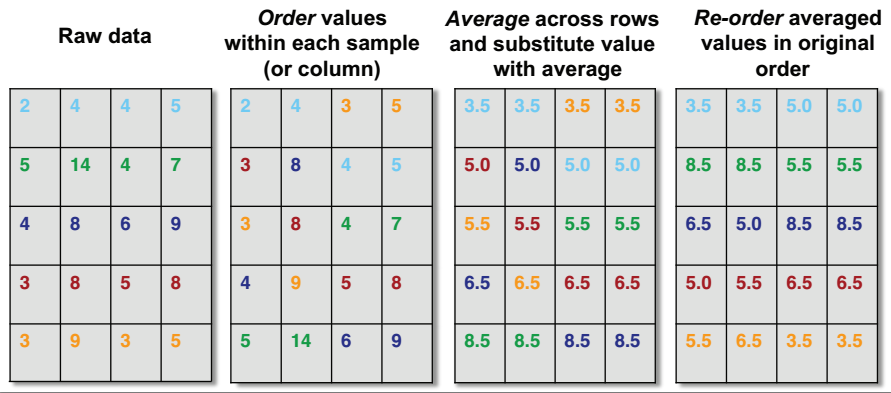
\includegraphics[width=0.8\linewidth]{img/quant_norm} 

}

\caption{Quantile Normalisation from \href{https://twitter.com/rafalab/status/545586012219772928?ref_src=twsrc\%5Etfw}{Rafael Irizarry's tweet}.}\label{fig:quant-norm}
\end{figure}

These result of quantile normalisation is that our distributions become
statisitcally identitical, which we can see by plotting the densities of the
normalized data. As shown in Figure \ref{fig:compare-normalisation} the distributions
all overlay.

We do this by creating a \protect\hyperlink{function-anatomy}{function}. This takes a data
frame as the arguement and pefrorms the steps described to iterate through
the data frame.

The code below is probably quite tricky to understand if
you've not seen \texttt{map} functions before, but they enable a function such as \texttt{rank}
or \texttt{sort} to be used on each column iteratively. What's important here is
to understand the aim, even if understanding the code requires some more reading.
You can read about \href{http://r4ds.had.co.nz/iteration.html\#the-map-functions}{map functions in R4DS}.

\begin{Shaded}
\begin{Highlighting}[]
\CommentTok{# Quantile normalisation : the aim is to give different distributions the}
\CommentTok{# same statistical properties}
\NormalTok{quantile_normalisation <-}\StringTok{ }\ControlFlowTok{function}\NormalTok{(df)\{}
  
  \CommentTok{# Find rank of values in each column}
\NormalTok{  df_rank <-}\StringTok{ }\KeywordTok{map_df}\NormalTok{(df,rank,}\DataTypeTok{ties.method=}\StringTok{"average"}\NormalTok{)}
  \CommentTok{# Sort observations in each column from lowest to highest }
\NormalTok{  df_sorted <-}\StringTok{ }\KeywordTok{map_df}\NormalTok{(df,sort)}
  \CommentTok{# Find row mean on sorted columns}
\NormalTok{  df_mean <-}\StringTok{ }\KeywordTok{rowMeans}\NormalTok{(df_sorted)}
  
  \CommentTok{# Function for substiting mean values according to rank }
\NormalTok{  index_to_mean <-}\StringTok{ }\ControlFlowTok{function}\NormalTok{(my_index, my_mean)\{}
    \KeywordTok{return}\NormalTok{(my_mean[my_index])}
\NormalTok{  \}}
  
  \CommentTok{# Replace value in each column with mean according to rank }
\NormalTok{  df_final <-}\StringTok{ }\KeywordTok{map_df}\NormalTok{(df_rank,index_to_mean, }\DataTypeTok{my_mean=}\NormalTok{df_mean)}
  
  \KeywordTok{return}\NormalTok{(df_final)}
\NormalTok{\}}
\end{Highlighting}
\end{Shaded}

The normalisation function is used by piping \texttt{dat\_tidy} first to \texttt{select} to
exclude the first two columns with the protein accession and description in, and
then to the normalisation function. We re-bind the protein accession and description afterwards from \texttt{dat\_tidy} by piping the output to \texttt{bind\_cols()}.

\begin{Shaded}
\begin{Highlighting}[]
\NormalTok{dat_norm <-}\StringTok{ }\NormalTok{dat_tidy }\OperatorTok\StringTok{ }\KeywordTok{select}\NormalTok{(}\OperatorTok{-}\KeywordTok{c}\NormalTok{(protein_accession}\OperatorTok{:}\NormalTok{protein_description)) }\OperatorTok\StringTok{ }
\StringTok{  }\KeywordTok{quantile_normalisation}\NormalTok{() }\OperatorTok\StringTok{ }
\StringTok{  }\KeywordTok{bind_cols}\NormalTok{(dat_tidy[,}\DecValTok{1}\OperatorTok{:}\DecValTok{2}\NormalTok{],.)}
\end{Highlighting}
\end{Shaded}




\begin{figure}

{\centering 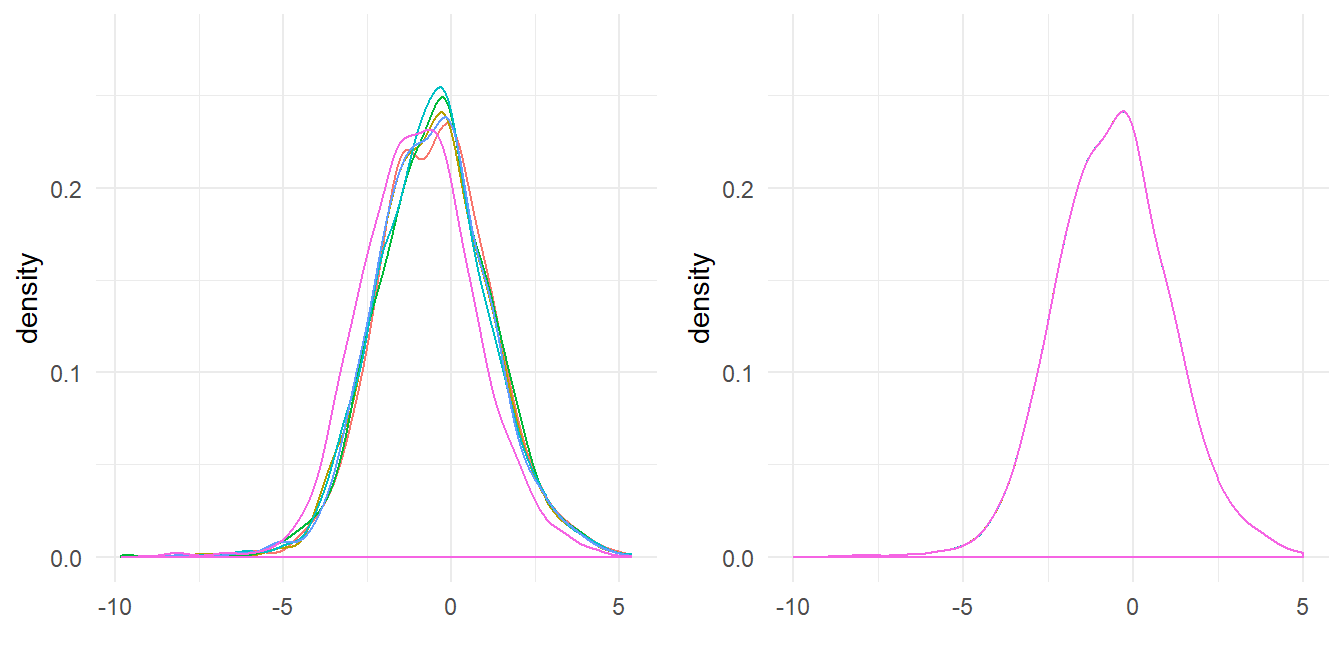
\includegraphics[width=0.8\linewidth]{bspr-workshop-2018_files/figure-latex/compare-normalisation-1} 

}

\caption{Comparison of the protein distributions before normalization (left)
and after quantile normalization (right).}\label{fig:compare-normalisation}
\end{figure}

\hypertarget{hypothesis-testing-with-the-t-test}{%
\section{Hypothesis testing with the t-test}\label{hypothesis-testing-with-the-t-test}}

Having removed missing values and normalised the data, we can consider our
hypothesis: treatement changes the amount of protein we observe in the cells.

In practice then, what we would like to know is whether the mean value for each
protein in our control and treatment assays differs due to chance or due a
real effect. We therefore need to calculate the difference for each protein
between treatment and control, and the probability that any difference occurs
due to chance. This is what the p-value from the output of a
t-test seeks to do. We need to perform 1145 t-tests.

\textbf{Note} There are biocondutor packages that contain functions written to do
this. However as a learning exercise we are going to work through the problem.

Here I assume the reader is familiar with t-tests, but just to re-cap some
important points:

\begin{itemize}
\item
  We assume that the true population from which our data samples are
  indpendent, identically distributed and follow a normal distribution. This is
  not in fact true in practice, but t-test is robust to this assumption.
\item
  We assume unequal variances between the control and treatment for each protein. Hence we will perform a Welch's t-test for unequal variances.
\item
  We don't know whether the effect of the treatment is to increase or decrease
  the concentration of the protein, hence we will perform a two-sided t-test.
\item
  The observations for the proteins are for proteins of the same type but from
  independent experiments, rather than observations of the same individuals
  before and after treatment. Hence we test the observations as unpaired samples.
\end{itemize}

In R we use the base function \texttt{t.test} to perform Welch Two Sample t-test and
this outputs the p-values we need for each protein. However, the challenge here
is that our data has three observations for each condition for each protein,
hence we need to group the observations for each protein according to the
experimental condition as inputs to each t-test.

We're going to follow what is called the \emph{split-apply-combine} approach to deal
with this problem:

\begin{enumerate}
\def\labelenumi{\arabic{enumi}.}
\tightlist
\item
  Split the data into control and treatment groups.
\item
  Apply the t-test function to each protein using the grouped inputs and
  store the p-value.
\item
  Combine all the p-values for each protein into a single vector.
\end{enumerate}

To this end I've created a function called \texttt{t\_test} that takes a data frame
and two group vectors as inputs. It splits the data into \texttt{x} and \texttt{y} by
subsetting the the data frame according to the columns defined by the groups.
The extra steps here are that the subset data has to be unlisted and converted
to numeric type for input to the \texttt{t.test} function. We then perform the t-test,
which will calculate the mean of \texttt{x} and \texttt{y} and store the result in a new
object, and finally the function creates a data frame with a single variable\texttt{p\_val} which is then returned as the function output.

\begin{Shaded}
\begin{Highlighting}[]
\CommentTok{# T-test function for multiple experiments}
\NormalTok{t_test <-}\StringTok{ }\ControlFlowTok{function}\NormalTok{(dt,grp1,grp2)\{}
  \CommentTok{# Subset control group and convert to numeric}
\NormalTok{  x <-}\StringTok{ }\NormalTok{dt[grp1] }\OperatorTok\StringTok{ }\NormalTok{unlist }\OperatorTok\StringTok{ }\KeywordTok{as.numeric}\NormalTok{()}
  \CommentTok{# Subset treatment group and convert to numeric}
\NormalTok{  y <-}\StringTok{ }\NormalTok{dt[grp2] }\OperatorTok\StringTok{ }\NormalTok{unlist }\OperatorTok\StringTok{ }\KeywordTok{as.numeric}\NormalTok{()}
  \CommentTok{# Perform t-test using the mean of x and y}
\NormalTok{  result <-}\StringTok{ }\KeywordTok{t.test}\NormalTok{(x, y)}
  \CommentTok{# Extract p-values from the results}
\NormalTok{  p_vals <-}\StringTok{ }\KeywordTok{tibble}\NormalTok{(}\DataTypeTok{p_val =}\NormalTok{ result}\OperatorTok{$}\NormalTok{p.value)}
  \CommentTok{# Return p-values}
  \KeywordTok{return}\NormalTok{(p_vals)}
\NormalTok{\} }
\end{Highlighting}
\end{Shaded}

To use the \texttt{t\_test} function to perform many t-tests and not just one t-test, we
need to pass our \texttt{t\_test} function as an arguement to another function.

This probably seems quite confusing, but the point here is that we want to loop
through every row in our table, and group the three control and three treatment
columns separately. Our \texttt{t\_test} function deals with the latter problem, and
by passing it to \texttt{adply} from the \texttt{plyr} package we can loop through each row
and it adds the calculated p-values to our original table.

Concretely then, \texttt{adply} takes an array and applies the \texttt{t\_test} function to
each row and we supply the column group indices arguments to the \texttt{t\_test}
funcition. Here the indicies are columns 3 to 5 for the control experiments and
columns 6 to 8 for the treatment functions. The function returns the input
data with an additional corresponding p-value column. \textbf{Note} I've piped
the output to \texttt{as.tibble()} to transform the data.frame output of \texttt{adply} to
tibble form to prevent errors that can occur if we try to bind data frames
and tibbles.

An important point here is that we can use this function for any number of
columns and rows providing our data is in the same tidy form by changing the
grouping indices.

\begin{Shaded}
\begin{Highlighting}[]
\CommentTok{# Apply t-test function to data using plyr adply}
\CommentTok{#  .margins = 1, slice by rows, .fun = t_test plus t_test arguements}
\NormalTok{dat_pvals <-}\StringTok{ }\NormalTok{plyr}\OperatorTok{::}\KeywordTok{adply}\NormalTok{(dat_norm,}\DataTypeTok{.margins =} \DecValTok{1}\NormalTok{, }\DataTypeTok{.fun =}\NormalTok{ t_test, }
                \DataTypeTok{grp1 =} \KeywordTok{c}\NormalTok{(}\DecValTok{3}\OperatorTok{:}\DecValTok{5}\NormalTok{), }\DataTypeTok{grp2 =} \KeywordTok{c}\NormalTok{(}\DecValTok{6}\OperatorTok{:}\DecValTok{8}\NormalTok{)) }\OperatorTok\StringTok{ }\KeywordTok{as.tibble}\NormalTok{()}
\end{Highlighting}
\end{Shaded}

\begin{verbatim}
## Warning: `as.tibble()` is deprecated, use `as_tibble()` (but mind the new semantics).
## This warning is displayed once per session.
\end{verbatim}

To check our function, here's a comparision of calculating the first protein
p-value as a single t-test as shown in the following code and the output of
the function.

\begin{Shaded}
\begin{Highlighting}[]
\CommentTok{# Perform t-test on first protein}
\KeywordTok{t.test}\NormalTok{(}\KeywordTok{as.numeric}\NormalTok{(dat_norm[}\DecValTok{1}\NormalTok{,}\DecValTok{3}\OperatorTok{:}\DecValTok{5}\NormalTok{]),}
                    \KeywordTok{as.numeric}\NormalTok{(dat_norm[}\DecValTok{1}\NormalTok{,}\DecValTok{6}\OperatorTok{:}\DecValTok{8}\NormalTok{]))}\OperatorTok{$}\NormalTok{p.value}
\end{Highlighting}
\end{Shaded}

\begin{tabular}{rr}
\toprule
t\_test p-val & t.test p-val\\
\midrule
0.0927 & 0.0927\\
\bottomrule
\end{tabular}

We can plot a histogram of the p-values:

\begin{Shaded}
\begin{Highlighting}[]
\CommentTok{# Plot histogram}
\NormalTok{dat_pvals }\OperatorTok\StringTok{ }
\StringTok{  }\KeywordTok{ggplot}\NormalTok{(}\KeywordTok{aes}\NormalTok{(p_val)) }\OperatorTok{+}\StringTok{ }
\StringTok{  }\KeywordTok{geom_histogram}\NormalTok{(}\DataTypeTok{binwidth =} \FloatTok{0.05}\NormalTok{, }
           \DataTypeTok{boundary =} \FloatTok{0.5}\NormalTok{, }
           \DataTypeTok{fill =} \StringTok{"darkblue"}\NormalTok{,}
           \DataTypeTok{colour =} \StringTok{"white"}\NormalTok{) }\OperatorTok{+}
\StringTok{  }\KeywordTok{xlab}\NormalTok{(}\StringTok{"p-value"}\NormalTok{) }\OperatorTok{+}
\StringTok{  }\KeywordTok{ylab}\NormalTok{(}\StringTok{"Frequency"}\NormalTok{) }\OperatorTok{+}
\StringTok{  }\KeywordTok{theme_minimal}\NormalTok{()}
\end{Highlighting}
\end{Shaded}

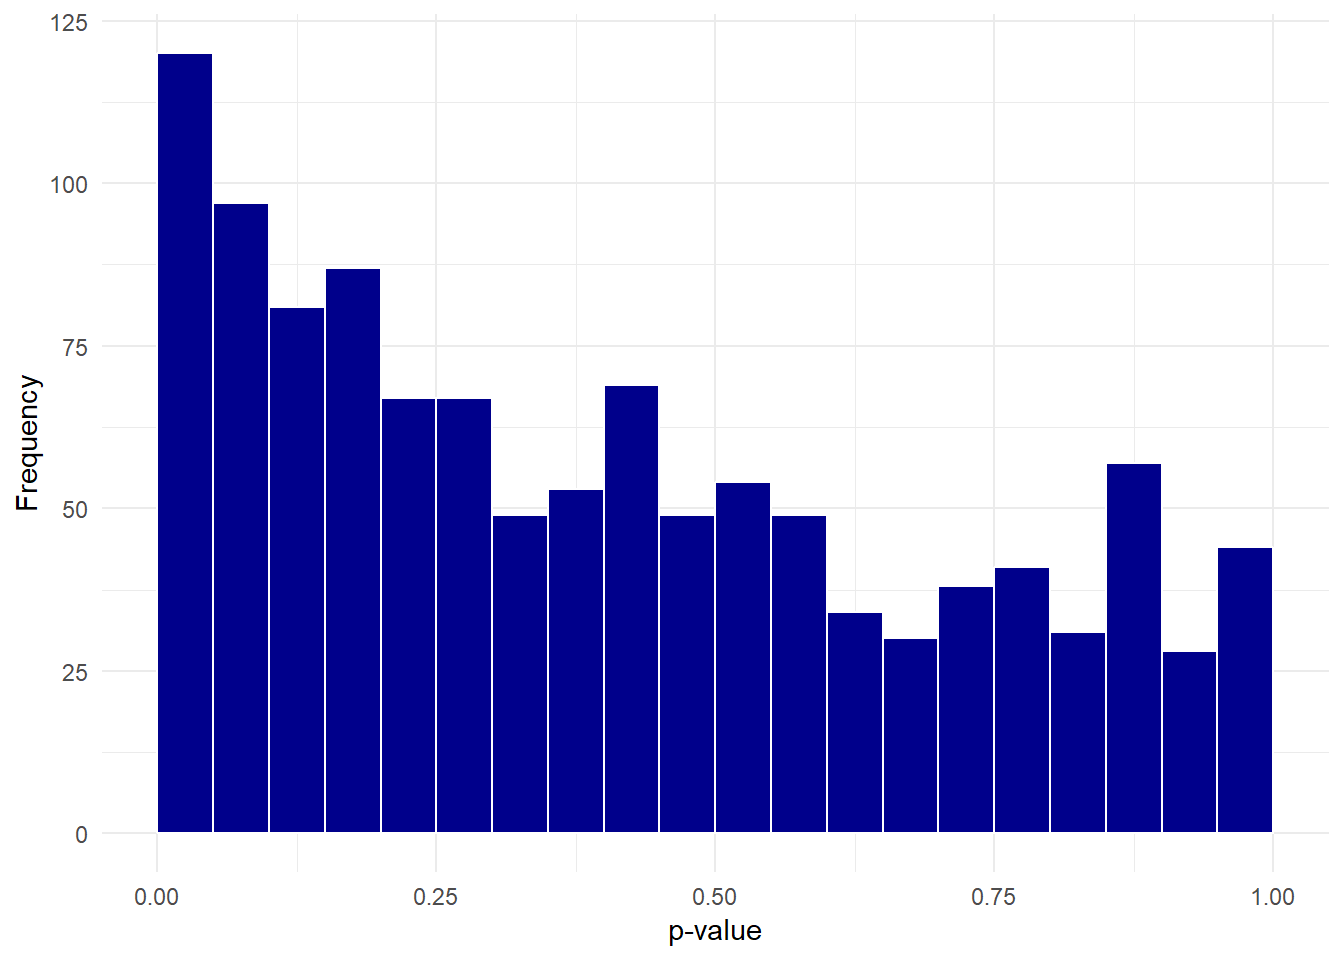
\includegraphics{bspr-workshop-2018_files/figure-latex/p-val-plot-1.pdf}

\hypertarget{calculating-fold-change}{%
\section{Calculating fold change}\label{calculating-fold-change}}

To perform log transformation of the observations for each protein we take our
data and use select to exlude the columns of character vectors and the pipe the
output to \texttt{log2()} and use the pipe again to create a data frame.

Then we use \texttt{bind\_cols} to bind the first two columns of \texttt{dat\_pvals} followed
by \texttt{dat\_log} and the last column of \texttt{dat\_pvals}. This maintains the original
column order.

\begin{Shaded}
\begin{Highlighting}[]
\CommentTok{# Select columns and log data}
\NormalTok{dat_log <-}\StringTok{ }\NormalTok{dat_pvals }\OperatorTok\StringTok{ }
\StringTok{  }\KeywordTok{select}\NormalTok{(}\OperatorTok{-}\KeywordTok{c}\NormalTok{(protein_accession,protein_description,p_val)) }\OperatorTok\StringTok{ }
\StringTok{  }\KeywordTok{log2}\NormalTok{()}

\CommentTok{# Bind columns to create transformed data frame}
\NormalTok{dat_combine <-}\StringTok{ }\KeywordTok{bind_cols}\NormalTok{(dat_pvals[,}\KeywordTok{c}\NormalTok{(}\DecValTok{1}\OperatorTok{:}\DecValTok{2}\NormalTok{)], dat_log, dat_pvals[,}\DecValTok{9}\NormalTok{]) }
\end{Highlighting}
\end{Shaded}

The log fold change is then the difference between the log mean control and
log mean treatment values. By use of grouping by the protein accession we
can then use \texttt{mutate} to create new variables that calculate the mean values
and then calculate the \texttt{log\_fc}. Whilst we're about it, we can also calculate
a -log10(p-value). As with fold change, transforming the p-value on a log10
scale means that a p-value of 0.05 or below is transformed to 1.3 or above and
a p-value of 0.01 is equal to 2.

\begin{Shaded}
\begin{Highlighting}[]
\NormalTok{dat_fc <-}\StringTok{ }\NormalTok{dat_combine }\OperatorTok\StringTok{ }
\StringTok{  }\KeywordTok{group_by}\NormalTok{(protein_accession) }\OperatorTok\StringTok{ }
\StringTok{  }\KeywordTok{mutate}\NormalTok{(}\DataTypeTok{mean_control =} \KeywordTok{mean}\NormalTok{(}\KeywordTok{c}\NormalTok{(control_}\DecValTok{1}\NormalTok{,}
\NormalTok{                               control_}\DecValTok{2}\NormalTok{,}
\NormalTok{                               control_}\DecValTok{3}\NormalTok{)),}
                             \DataTypeTok{mean_treatment=} \KeywordTok{mean}\NormalTok{(}\KeywordTok{c}\NormalTok{(treatment_}\DecValTok{1}\NormalTok{,}
\NormalTok{                                                    treatment_}\DecValTok{2}\NormalTok{,}
\NormalTok{                                                    treatment_}\DecValTok{3}\NormalTok{)),}
         \DataTypeTok{log_fc =}\NormalTok{ mean_control }\OperatorTok{-}\StringTok{ }\NormalTok{mean_treatment,}
         \DataTypeTok{log_pval =} \DecValTok{-1}\OperatorTok{*}\KeywordTok{log10}\NormalTok{(p_val))}
\end{Highlighting}
\end{Shaded}

The next step is not necessary, but for ease of viewing we subset \texttt{dat\_fc} to
create a new data frame called \texttt{dat\_tf} that contains only four variables.
We could potentially write this to a csv file for sharing.

\begin{Shaded}
\begin{Highlighting}[]
\CommentTok{# Final transformed data}
\NormalTok{dat_tf <-}\StringTok{ }\NormalTok{dat_fc }\OperatorTok\StringTok{ }\KeywordTok{select}\NormalTok{(protein_accession,}
\NormalTok{                            protein_description,}
\NormalTok{                            log_fc, log_pval)}
\end{Highlighting}
\end{Shaded}

Let's look at the head of the final table:

\begin{tabular}{llrr}
\toprule
protein\_accession & protein\_description & log\_fc & log\_pval\\
\midrule
VATA\_HUMAN\_P38606 & V-type proton ATPase catalytic subunit A OS=Homo sapiens GN=ATP6V1A PE=1 SV=2 & 0.3687886 & 1.0327506\\
RL35A\_HUMAN\_P18077 & 60S ribosomal protein L35a OS=Homo sapiens GN=RPL35A PE=1 SV=2 & -0.2505780 & 1.1400318\\
MYH10\_HUMAN\_P35580 & Myosin-10 OS=Homo sapiens GN=MYH10 PE=1 SV=3 & 0.3838733 & 0.0056494\\
RHOG\_HUMAN\_P84095 & Rho-related GTP-binding protein RhoG OS=Homo sapiens GN=RHOG PE=1 SV=1 & -0.3417452 & 0.3775483\\
PSA1\_HUMAN\_P25786 & Proteasome subunit alpha type-1 OS=Homo sapiens GN=PSMA1 PE=1 SV=1 & 0.0371316 & 0.0920101\\
\bottomrule
\end{tabular}

\hypertarget{visualising-the-transformed-data}{%
\section{Visualising the transformed data}\label{visualising-the-transformed-data}}

Plotting a histogram of the log fold change gives an indication of whether the
treatment has an effect on the cells. Most values are close to zero, but there
are some observations far above and below zero suggesting the treatment
does have an effect.



\begin{Shaded}
\begin{Highlighting}[]
\CommentTok{# Plot a histogram to look at the distribution.}
\NormalTok{dat_tf }\OperatorTok
\StringTok{  }\KeywordTok{ggplot}\NormalTok{(}\KeywordTok{aes}\NormalTok{(log_fc)) }\OperatorTok{+}\StringTok{ }
\StringTok{  }\KeywordTok{geom_histogram}\NormalTok{(}\DataTypeTok{binwidth =} \FloatTok{0.5}\NormalTok{,}
                 \DataTypeTok{boundary =} \FloatTok{0.5}\NormalTok{,}
           \DataTypeTok{fill =} \StringTok{"darkblue"}\NormalTok{,}
           \DataTypeTok{colour =} \StringTok{"white"}\NormalTok{) }\OperatorTok{+}
\StringTok{  }\KeywordTok{xlab}\NormalTok{(}\StringTok{"log2 fold change"}\NormalTok{) }\OperatorTok{+}
\StringTok{  }\KeywordTok{ylab}\NormalTok{(}\StringTok{"Frequency"}\NormalTok{) }\OperatorTok{+}
\StringTok{  }\KeywordTok{theme_minimal}\NormalTok{()}
\end{Highlighting}
\end{Shaded}

\begin{figure}

{\centering 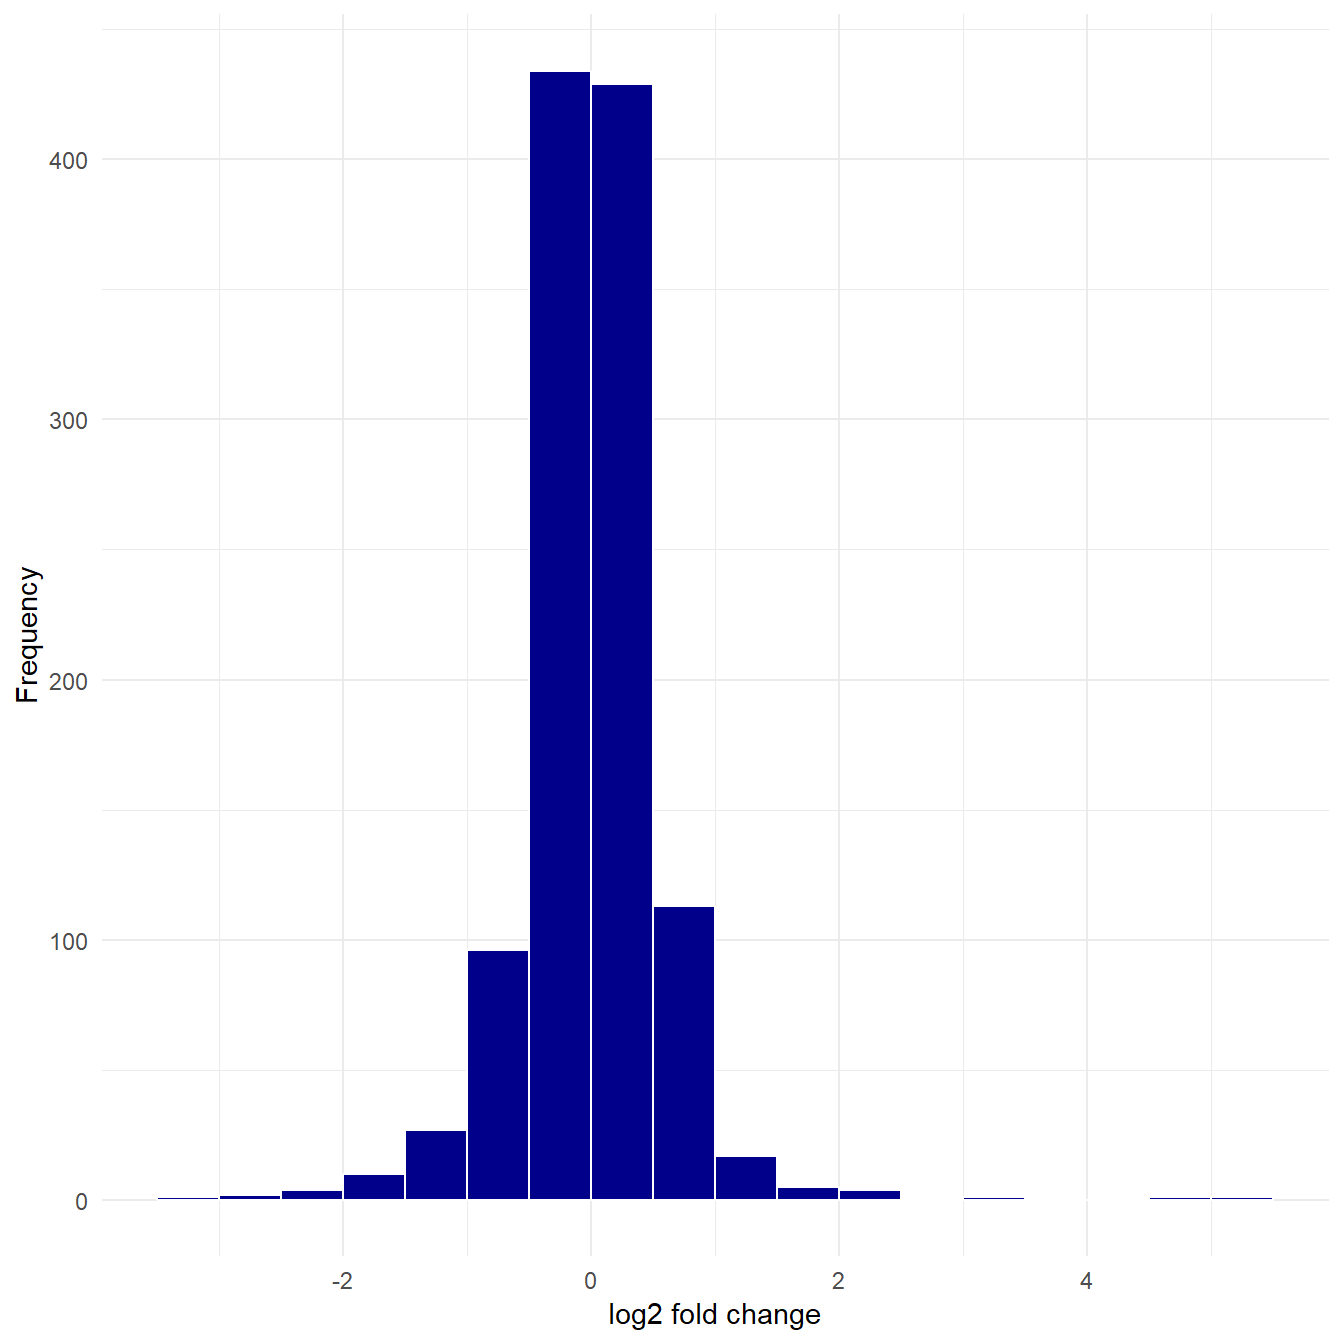
\includegraphics[width=0.8\linewidth]{bspr-workshop-2018_files/figure-latex/log-fc-1} 

}

\caption{Histogram of log fold change.}\label{fig:log-fc}
\end{figure}

However, we don't know if these fold changes are dueto chance or not, which is
why we calculated the p-values. A volcano plot will include the p-value
information.

\hypertarget{volcano-plot}{%
\section{Volcano plot}\label{volcano-plot}}

A volcano plot is a plot of the log fold change in the observation between two
conditions on the x-axis, for example the protein expression between treatment
and control conditions. On the y-axis is the corresponding p-value for each
observation, representing the likelihood that an observed change
is due to the different conditions rather than arising from a natural variation
in the fold change that might be observed if we performed many replications of
the experiment.

The aim of a volcano plot is to enable the viewer to quickly see the effect
(if any) of an experiment with two conditions on many species (i.e.~proteins)
in terms of both an increase and decrease of the observed value.

Like all plots it has it's good and bad points, namely it's good that we can
visualise a lot of complex information in one plot. However this is also it's
main weakness, it's rather complicated to understand in one glance.

\begin{Shaded}
\begin{Highlighting}[]
\NormalTok{dat_tf }\OperatorTok\StringTok{ }\KeywordTok{ggplot}\NormalTok{(}\KeywordTok{aes}\NormalTok{(log_fc,log_pval)) }\OperatorTok{+}\StringTok{ }\KeywordTok{geom_point}\NormalTok{()}
\end{Highlighting}
\end{Shaded}

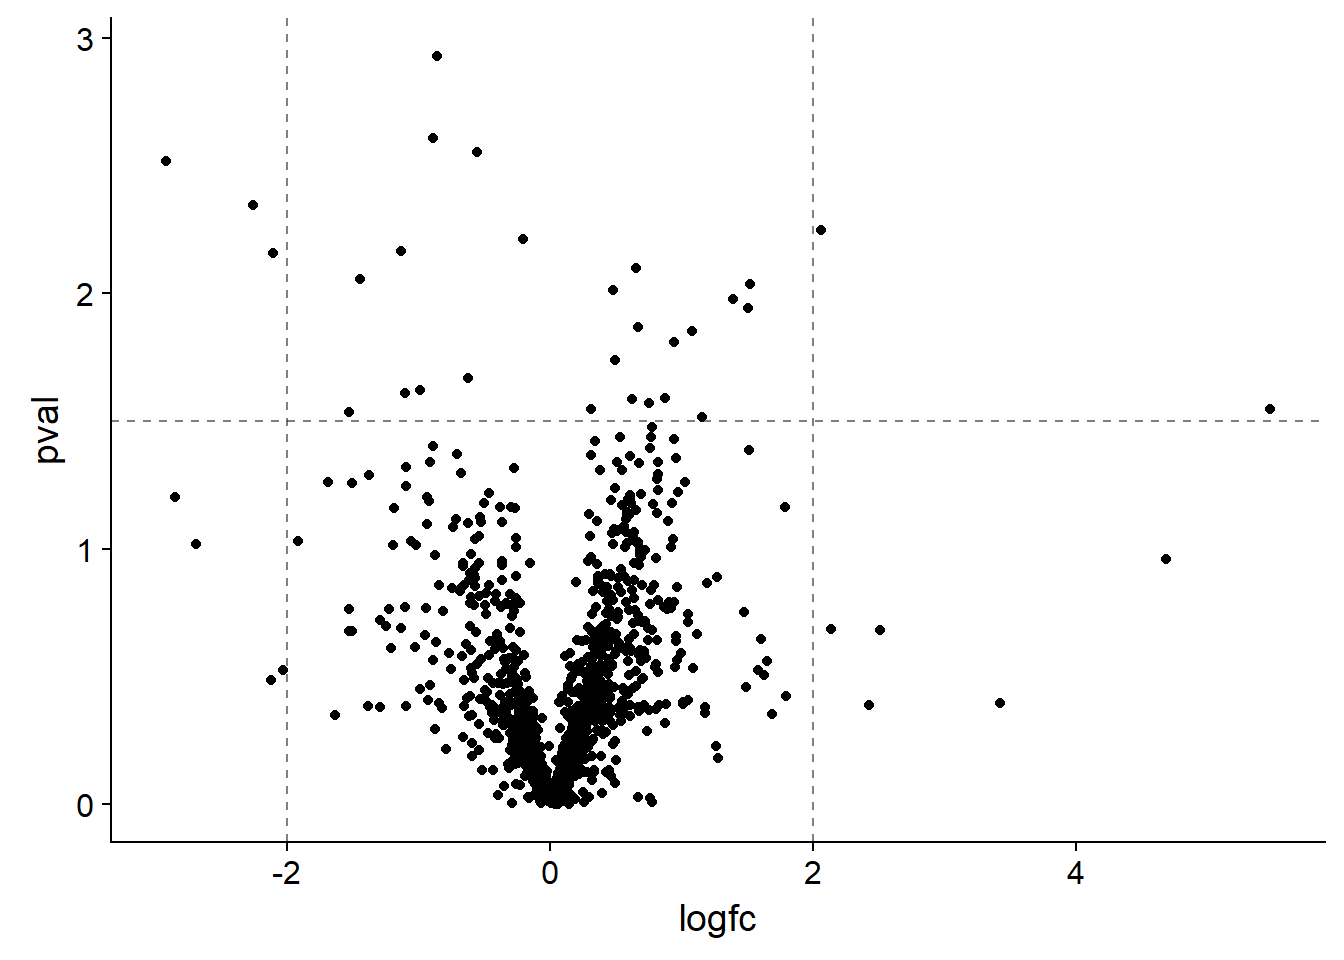
\includegraphics{bspr-workshop-2018_files/figure-latex/volcano-plot-1.pdf}

However it would be much more useful with some extra formatting, so the code
below shows one way to transform the data to include a threshold which can
then be used by ggplot to create an additional aesthetic. The code below
also includes some extra formatiing which the reader can explore.



\begin{Shaded}
\begin{Highlighting}[]
\NormalTok{dat_tf }\OperatorTok
\StringTok{  }\CommentTok{# Add a threhold for significant observations}
\StringTok{  }\KeywordTok{mutate}\NormalTok{(}\DataTypeTok{threshold =} \KeywordTok{if_else}\NormalTok{(log_fc }\OperatorTok{>=}\StringTok{ }\DecValTok{2} \OperatorTok{&}\StringTok{ }\NormalTok{log_pval }\OperatorTok{>=}\StringTok{ }\FloatTok{1.3} \OperatorTok{|}
\StringTok{                               }\NormalTok{log_fc }\OperatorTok{<=}\StringTok{ }\DecValTok{-2} \OperatorTok{&}\StringTok{ }\NormalTok{log_pval }\OperatorTok{>=}\StringTok{ }\FloatTok{1.3}\NormalTok{,}\StringTok{"A"}\NormalTok{, }\StringTok{"B"}\NormalTok{)) }\OperatorTok
\StringTok{  }\CommentTok{# Plot with points coloured according to the threshold}
\StringTok{  }\KeywordTok{ggplot}\NormalTok{(}\KeywordTok{aes}\NormalTok{(log_fc,log_pval, }\DataTypeTok{colour =}\NormalTok{ threshold)) }\OperatorTok{+}
\StringTok{  }\KeywordTok{geom_point}\NormalTok{(}\DataTypeTok{alpha =} \FloatTok{0.5}\NormalTok{) }\OperatorTok{+}\StringTok{ }\CommentTok{# Alpha sets the transparency of the points}
\StringTok{  }\CommentTok{# Add dotted lines to indicate the threshold, semi-transparent}
\StringTok{  }\KeywordTok{geom_hline}\NormalTok{(}\DataTypeTok{yintercept =} \FloatTok{1.3}\NormalTok{, }\DataTypeTok{linetype =} \DecValTok{2}\NormalTok{, }\DataTypeTok{alpha =} \FloatTok{0.5}\NormalTok{) }\OperatorTok{+}\StringTok{ }
\StringTok{  }\KeywordTok{geom_vline}\NormalTok{(}\DataTypeTok{xintercept =} \DecValTok{2}\NormalTok{, }\DataTypeTok{linetype =} \DecValTok{2}\NormalTok{, }\DataTypeTok{alpha =} \FloatTok{0.5}\NormalTok{) }\OperatorTok{+}
\StringTok{  }\KeywordTok{geom_vline}\NormalTok{(}\DataTypeTok{xintercept =} \DecValTok{-2}\NormalTok{, }\DataTypeTok{linetype =} \DecValTok{2}\NormalTok{, }\DataTypeTok{alpha =} \FloatTok{0.5}\NormalTok{) }\OperatorTok{+}
\StringTok{  }\CommentTok{# Set the colour of the points}
\StringTok{  }\KeywordTok{scale_colour_manual}\NormalTok{(}\DataTypeTok{values =} \KeywordTok{c}\NormalTok{(}\StringTok{"A"}\NormalTok{=}\StringTok{ "red"}\NormalTok{, }\StringTok{"B"}\NormalTok{=}\StringTok{ "black"}\NormalTok{)) }\OperatorTok{+}
\StringTok{  }\KeywordTok{xlab}\NormalTok{(}\StringTok{"log2 fold change"}\NormalTok{) }\OperatorTok{+}\StringTok{ }\KeywordTok{ylab}\NormalTok{(}\StringTok{"-log10 p-value"}\NormalTok{) }\OperatorTok{+}\StringTok{ }\CommentTok{# Relabel the axes}
\StringTok{  }\KeywordTok{theme_minimal}\NormalTok{() }\OperatorTok{+}\StringTok{ }\CommentTok{# Set the theme}
\StringTok{  }\KeywordTok{theme}\NormalTok{(}\DataTypeTok{legend.position=}\StringTok{"none"}\NormalTok{) }\CommentTok{# Hide the legend}
\end{Highlighting}
\end{Shaded}

\begin{figure}

{\centering 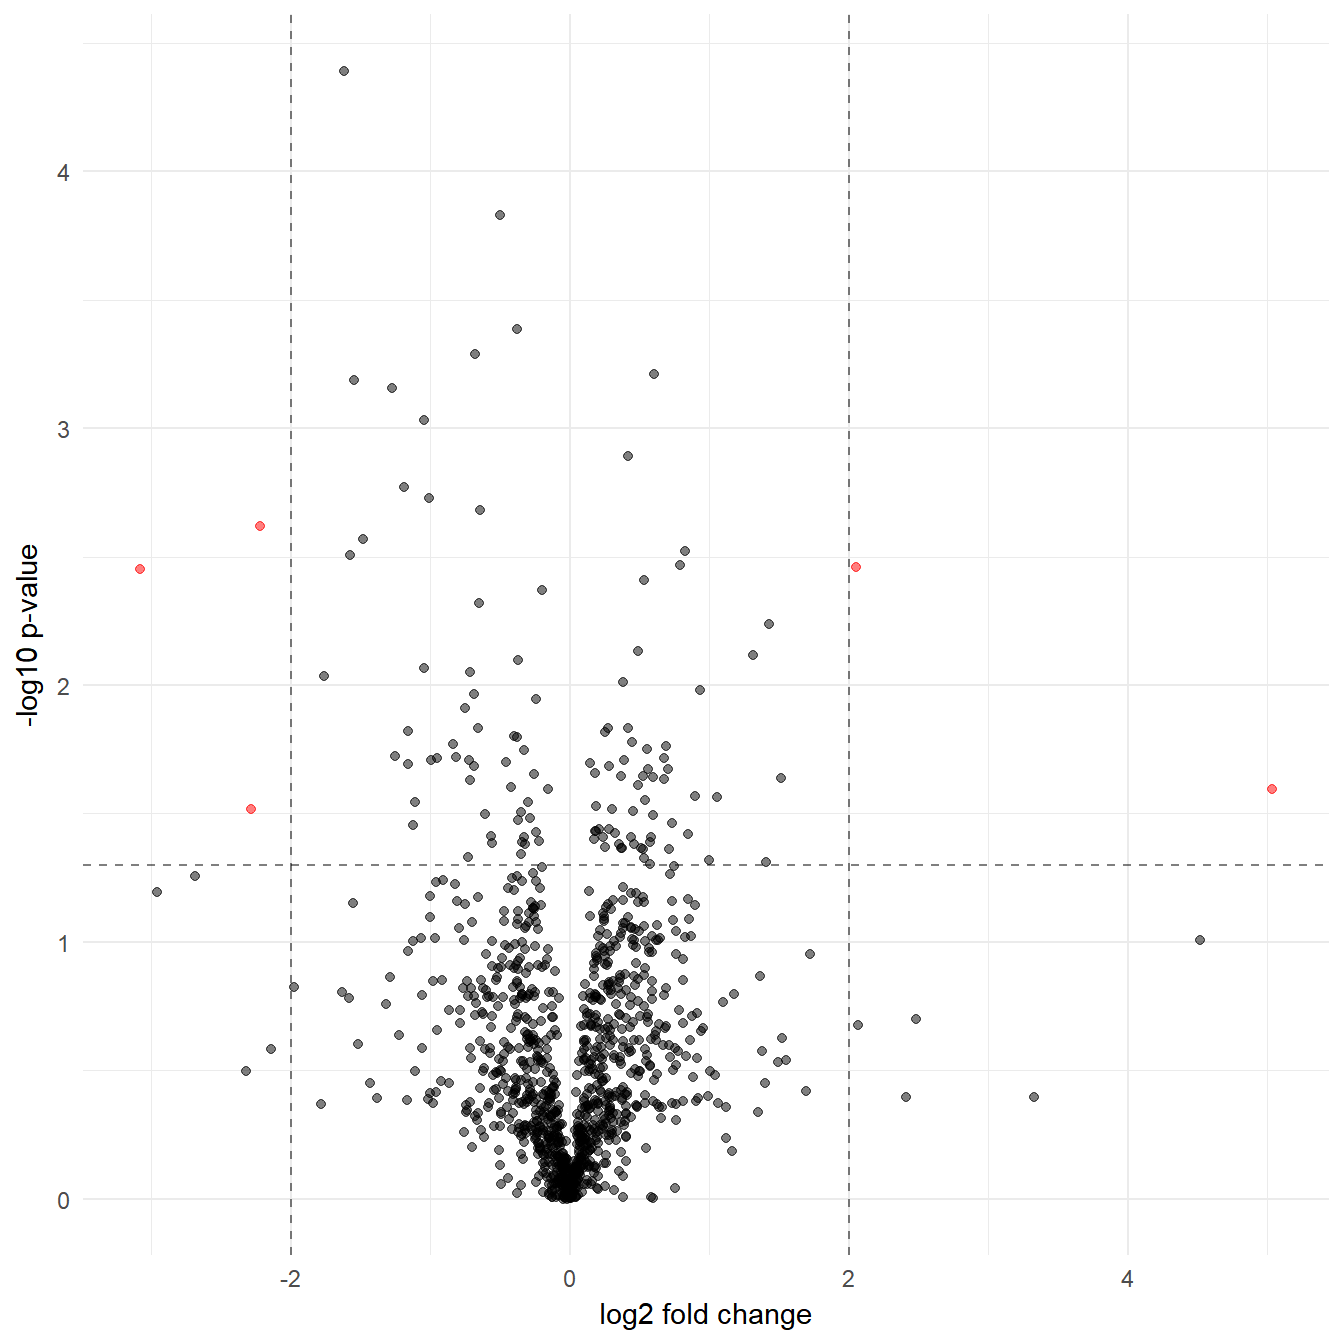
\includegraphics[width=0.8\linewidth]{bspr-workshop-2018_files/figure-latex/nice-vplot-1} 

}

\caption{A volcano plot with formatting to highlight the significant proteins}\label{fig:nice-vplot}
\end{figure}

\hypertarget{but-which-proteins-are-the-significant-observations}{%
\subsection{But which proteins are the significant observations?}\label{but-which-proteins-are-the-significant-observations}}

To extract the proteins in red in Figure \ref{fig:nice-vplot} we filter \texttt{dat\_tf}
according to our threshold and then create a new variable using the \texttt{str\_extract}
function used in Section \ref{mutate}.

\textbf{Note} We need to ungroup the data we grouped when calculating the log\_fc to
be able to select columns without keeping the grouping variable column too.

\begin{Shaded}
\begin{Highlighting}[]
\NormalTok{dat_tf }\OperatorTok
\StringTok{  }\CommentTok{# Filter for significant observations}
\StringTok{  }\KeywordTok{filter}\NormalTok{(log_pval }\OperatorTok{>=}\StringTok{ }\FloatTok{1.3} \OperatorTok{&}\StringTok{ }\NormalTok{(log_fc }\OperatorTok{>=}\StringTok{ }\DecValTok{2} \OperatorTok{|}\StringTok{ }\NormalTok{log_fc }\OperatorTok{<=}\StringTok{ }\DecValTok{-2}\NormalTok{)) }\OperatorTok\StringTok{ }
\StringTok{  }\CommentTok{# Get last six characters}
\StringTok{  }\KeywordTok{mutate}\NormalTok{(}\DataTypeTok{prot_id =} \KeywordTok{str_extract}\NormalTok{(protein_accession,}\StringTok{".\{6\}$"}\NormalTok{)) }\OperatorTok\StringTok{ }
\StringTok{  }\CommentTok{# Ungroup the data}
\StringTok{  }\KeywordTok{ungroup}\NormalTok{() }\OperatorTok\StringTok{ }
\StringTok{  }\CommentTok{# Select columns of interest}
\StringTok{  }\KeywordTok{select}\NormalTok{(prot_id,protein_description,log_fc,log_pval)}
\end{Highlighting}
\end{Shaded}

\begin{verbatim}
## # A tibble: 5 x 4
##   prot_id protein_description                               log_fc log_pval
##   <chr>   <chr>                                              <dbl>    <dbl>
## 1 Q02952  A-kinase anchor protein 12 OS=Homo sapiens GN=AK~  -2.29     1.52
## 2 O94808  Glutamine--fructose-6-phosphate aminotransferase~  -3.09     2.45
## 3 H7BYV1  Interferon-induced transmembrane protein 2 (Frag~   2.05     2.46
## 4 P06756  Integrin alpha-V OS=Homo sapiens GN=ITGAV PE=1 S~  -2.22     2.62
## 5 Q8TDI0  Chromodomain-helicase-DNA-binding protein 5 OS=H~   5.04     1.60
\end{verbatim}

\hypertarget{creating-a-heatmap}{%
\section{Creating a heatmap}\label{creating-a-heatmap}}

Here we'll create a heatmap using the \texttt{heatmap.2} function from the \texttt{gplots}
package and the \texttt{pheatmap} function from the \texttt{pheatmap} package.

To create a heatmap we need to perform a few more transformations:

\begin{enumerate}
\def\labelenumi{\arabic{enumi}.}
\item
  Filter the data according to a threshold of significance. This time we'll use
  a more relaxed log\_fc cut-off to ensure we have enough proteins to plot. At
  the same time we'll extract the protein ids as before.
\item
  We then have to transform our filtered data into a \texttt{matrix.data.frame} object
  for use with \texttt{pheatmap}. We name the rows with the protein ids
\item
  We'll use base R function \texttt{scale} to centre our log transformed data around zero. To do this per experiment we transpose the matrix as scale centres rows,
  and the flip the matrix back again.
\end{enumerate}

\begin{Shaded}
\begin{Highlighting}[]
\CommentTok{# Keep the same p-val cut-off, but relax the log_fc to 1 which represents a }
\CommentTok{# doubling}
\NormalTok{dat_filt <-}\StringTok{ }\NormalTok{dat_fc }\OperatorTok
\StringTok{  }\KeywordTok{filter}\NormalTok{(log_pval }\OperatorTok{>=}\StringTok{ }\FloatTok{1.3} \OperatorTok{&}\StringTok{ }\NormalTok{(log_fc }\OperatorTok{>=}\StringTok{ }\DecValTok{1} \OperatorTok{|}\StringTok{ }\NormalTok{log_fc }\OperatorTok{<=}\StringTok{ }\DecValTok{-1}\NormalTok{)) }\OperatorTok\StringTok{ }
\StringTok{  }\KeywordTok{mutate}\NormalTok{(}\DataTypeTok{prot_id =} \KeywordTok{str_extract}\NormalTok{(protein_accession,}\StringTok{".\{6\}$"}\NormalTok{))}

\CommentTok{# Convert to matrix data frame}
\NormalTok{dat_matrix <-}\StringTok{ }\KeywordTok{as.matrix.data.frame}\NormalTok{(dat_filt[,}\DecValTok{3}\OperatorTok{:}\DecValTok{8}\NormalTok{]) }
\CommentTok{# Name the rows with protein ids}
\KeywordTok{row.names}\NormalTok{(dat_matrix) <-}\StringTok{ }\NormalTok{dat_filt}\OperatorTok{$}\NormalTok{prot_id}
\CommentTok{# Transpose and scale the data to a mean of zero and sd of one}
\NormalTok{dat_scaled <-}\StringTok{ }\KeywordTok{scale}\NormalTok{(}\KeywordTok{t}\NormalTok{(dat_matrix)) }\OperatorTok\StringTok{ }\KeywordTok{t}\NormalTok{()}
\end{Highlighting}
\end{Shaded}

\hypertarget{calculating-similarity-and-clustering}{%
\subsection{Calculating similarity and clustering}\label{calculating-similarity-and-clustering}}

At this point we could just plot the data, but to understand what the heatmap
functions do to cluster the data, let's step through the process.

Our data here as log fold change in concentrations, but how do we group them?
The simplest thing to do is to turn the data into distances, as a measure of
similarity, where close things are similar and distant things are dissimilar.

The Euclidean distance \(d\) between a pair of observations \(x_i\) and \(y_i\) is defined as:

\(d = \sqrt{\sum{_i}(x_i - y_i)^2}\)

Lets calculate the distance between the columns in \texttt{dat\_scaled}.

In \texttt{dat\_scaled} the experiments are in the columns. In calculating the distance
is between the experiments for all the proteins in each experiment. What would
we expect?

We'd expect the controls to be close to each other and the treated to be close
to each other, right?

Let's do this in detail, for example the distance between \texttt{control\_1} and
\texttt{control\_2} is \texttt{sqrt(sum((dat\_scaled{[},1{]}\ -\ dat\_scaled{[},2{]})\^{}2))}.

This means we take the column 2 values from column 1 values, squaring the results
and summing them all to a single value and taking the square root to find the
linear distance between these rows, which is 3.26.

You can check this against the first value in \texttt{d1} that we calculate below in using \texttt{dist}.

We do the same for the proteins, but we don't know what to expect. Here's the
code for calculating both distance matrices

\begin{Shaded}
\begin{Highlighting}[]
\CommentTok{# Transpose the matrix to calculate distance between experiments, row-wise}
\NormalTok{d1 <-}\StringTok{ }\NormalTok{dat_scaled }\OperatorTok\StringTok{ }\KeywordTok{t}\NormalTok{() }\OperatorTok
\StringTok{  }\KeywordTok{dist}\NormalTok{(.,}\DataTypeTok{method =} \StringTok{"euclidean"}\NormalTok{, }\DataTypeTok{diag =} \OtherTok{FALSE}\NormalTok{, }\DataTypeTok{upper =} \OtherTok{FALSE}\NormalTok{)}
\CommentTok{# Calculate the distance between proteins row-wise }
\NormalTok{d2 <-}\StringTok{ }\NormalTok{dat_scaled }\OperatorTok
\StringTok{  }\KeywordTok{dist}\NormalTok{(.,}\DataTypeTok{method =} \StringTok{"euclidean"}\NormalTok{, }\DataTypeTok{diag =} \OtherTok{FALSE}\NormalTok{, }\DataTypeTok{upper =} \OtherTok{FALSE}\NormalTok{)}

\CommentTok{# Show the values for d1}
\KeywordTok{round}\NormalTok{(d1,}\DecValTok{2}\NormalTok{)}
\end{Highlighting}
\end{Shaded}

\begin{verbatim}
##             control_1 control_2 control_3 treatment_1 treatment_2
## control_2        3.26                                            
## control_3        3.20      3.27                                  
## treatment_1      8.97      8.60      8.65                        
## treatment_2      9.40      8.98      8.86        2.35            
## treatment_3      9.04      8.56      8.50        2.46        1.71
\end{verbatim}

Having calculated the distance matrices, we can cluster proteins and experiments
accordingly.

There are lots of flavours of clustering, and no clear way to say which is best.
Here we'll use the Ward criterion for clustering which attempts to minimise the
variance within clusters as it merges the data into clusters, using the distances
we've calculated. The data is merged from the bottom up (aka agglomeration)
adding data points to a cluster and splitting them according to the variance
criterion.

See Wikipedia for more detail:
\href{https://en.wikipedia.org/wiki/Hierarchical_clustering}{Hierarchical clustering}

\begin{Shaded}
\begin{Highlighting}[]
\CommentTok{# Clustering distance between experiments using Ward linkage}
\NormalTok{c1 <-}\StringTok{ }\KeywordTok{hclust}\NormalTok{(d1, }\DataTypeTok{method =} \StringTok{"ward.D2"}\NormalTok{, }\DataTypeTok{members =} \OtherTok{NULL}\NormalTok{)}
\CommentTok{# Clustering distance between proteins using Ward linkage}
\NormalTok{c2 <-}\StringTok{ }\KeywordTok{hclust}\NormalTok{(d2, }\DataTypeTok{method =} \StringTok{"ward.D2"}\NormalTok{, }\DataTypeTok{members =} \OtherTok{NULL}\NormalTok{)}
\end{Highlighting}
\end{Shaded}

Now lets look at the dendrograms made by
clustering our distance matrices \texttt{d1} and \texttt{d2}:



\begin{Shaded}
\begin{Highlighting}[]
\CommentTok{# Check clustering by plotting dendrograms}
\KeywordTok{par}\NormalTok{(}\DataTypeTok{mfrow=}\KeywordTok{c}\NormalTok{(}\DecValTok{2}\NormalTok{,}\DecValTok{1}\NormalTok{),}\DataTypeTok{cex=}\FloatTok{0.5}\NormalTok{) }\CommentTok{# Make 2 rows, 1 col plot frame and shrink labels}
\KeywordTok{plot}\NormalTok{(c1); }\KeywordTok{plot}\NormalTok{(c2) }\CommentTok{# Plot both cluster dendrograms}
\end{Highlighting}
\end{Shaded}

\begin{figure}

{\centering 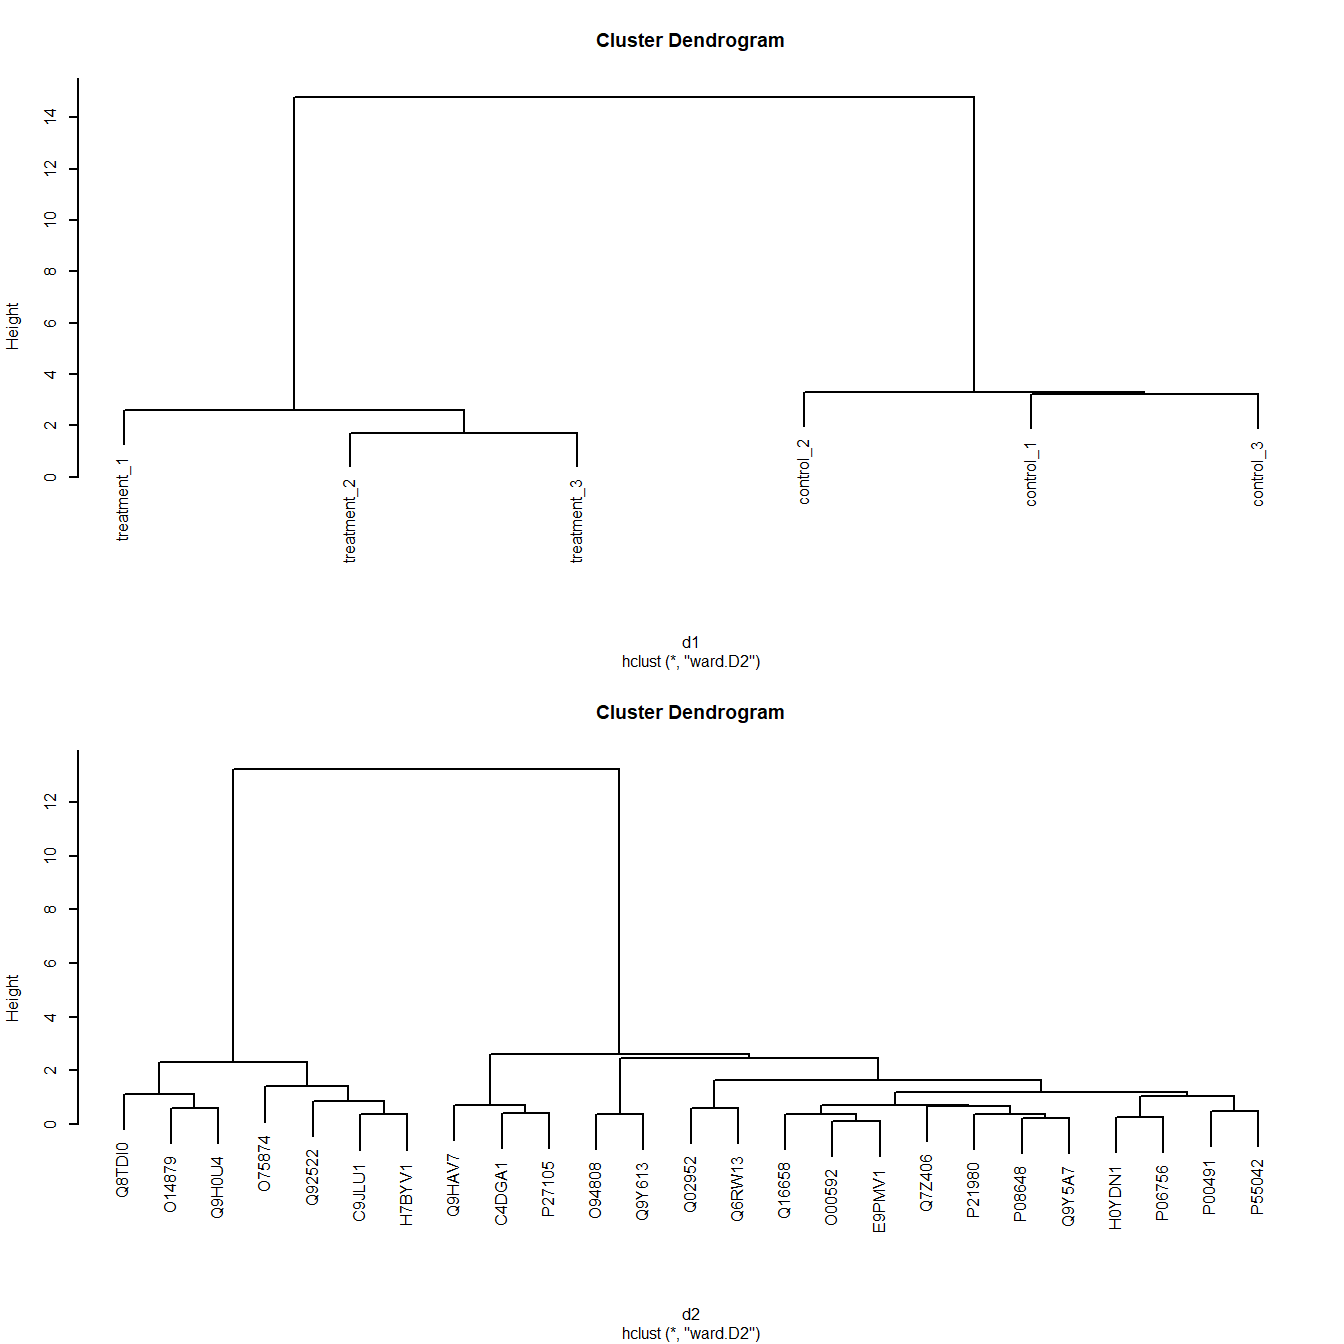
\includegraphics[width=0.8\linewidth]{bspr-workshop-2018_files/figure-latex/dendrograms-1} 

}

\caption{Dendrograms of Ward clustering of distance matrices}\label{fig:dendrograms}
\end{figure}

As we'd expect, Figure \ref{fig:dendrograms} shows the controls and treatments
cluster respectively.

\hypertarget{plotting-the-heatmap}{%
\subsection{Plotting the heatmap}\label{plotting-the-heatmap}}

The \texttt{heatmap.2} function from the \texttt{gplots} package will automatically perform
the distance calculation and clustering we performed, and it can also do
the scaling we did. It only requires the matrix as an input by default. It will
use a different clustering method by default.

However, as we've performed scaling and calculated the clusters, we can pass
them to heatmap function.

I'll leave it to the reader to explore all the options here, but the concept in
the code below to create Figure \ref{fig:heatmap2} is:

\begin{itemize}
\tightlist
\item
  Create a 25 increment blue/white/red colour pallette
\item
  Pipe \texttt{dat\_scaled} to a function that renames the colums
\item
  Pipe this to the \texttt{heatmap.2} function
\item
  Pass the clusters \texttt{c1} and \texttt{c2} to the plot
\item
  Change some aesthetics such as the colours, and the font sizes
\end{itemize}



\begin{Shaded}
\begin{Highlighting}[]
\CommentTok{# Set colours for heatmap, 25 increments}
\NormalTok{my_palette <-}\StringTok{ }\KeywordTok{colorRampPalette}\NormalTok{(}\KeywordTok{c}\NormalTok{(}\StringTok{"blue"}\NormalTok{,}\StringTok{"white"}\NormalTok{,}\StringTok{"red"}\NormalTok{))(}\DataTypeTok{n =} \DecValTok{25}\NormalTok{)}

\CommentTok{# Plot heatmap with heatmap.2}
\KeywordTok{par}\NormalTok{(}\DataTypeTok{cex.main=}\FloatTok{0.75}\NormalTok{) }\CommentTok{# Shrink title fonts on plot}
\NormalTok{dat_scaled }\OperatorTok\StringTok{ }
\StringTok{  }\CommentTok{# Rename the comlums}
\StringTok{  }\NormalTok{magrittr}\OperatorTok{::}\KeywordTok{set_colnames}\NormalTok{(}\KeywordTok{c}\NormalTok{(}\StringTok{"Ctl 1"}\NormalTok{, }\StringTok{"Ctl 2"}\NormalTok{, }\StringTok{"Ctl 3"}\NormalTok{,}
                                    \StringTok{"Trt 1"}\NormalTok{, }\StringTok{"Trt 2"}\NormalTok{, }\StringTok{"Trt 3"}\NormalTok{)) }\OperatorTok\StringTok{ }
\StringTok{  }\CommentTok{# Plot heatmap}
\StringTok{  }\NormalTok{gplots}\OperatorTok{::}\KeywordTok{heatmap.2}\NormalTok{(.,                     }\CommentTok{# Tidy, normalised data}
          \DataTypeTok{Colv=}\KeywordTok{as.dendrogram}\NormalTok{(c1),     }\CommentTok{# Experiments clusters in cols}
          \DataTypeTok{Rowv=}\KeywordTok{as.dendrogram}\NormalTok{(c2),     }\CommentTok{# Protein clusters in rows}
          \DataTypeTok{revC=}\OtherTok{TRUE}\NormalTok{,                  }\CommentTok{# Flip plot to match pheatmap}
          \DataTypeTok{density.info=}\StringTok{"histogram"}\NormalTok{,   }\CommentTok{# Plot histogram of data and colour key}
          \DataTypeTok{trace=}\StringTok{"none"}\NormalTok{,               }\CommentTok{# Turn of trace lines from heat map}
          \DataTypeTok{col =}\NormalTok{ my_palette,           }\CommentTok{# Use my colour scheme}
          \DataTypeTok{cexRow=}\FloatTok{0.6}\NormalTok{,}\DataTypeTok{cexCol=}\FloatTok{0.75}\NormalTok{)     }\CommentTok{# Amend row and column label fonts}
\end{Highlighting}
\end{Shaded}

\begin{figure}

{\centering 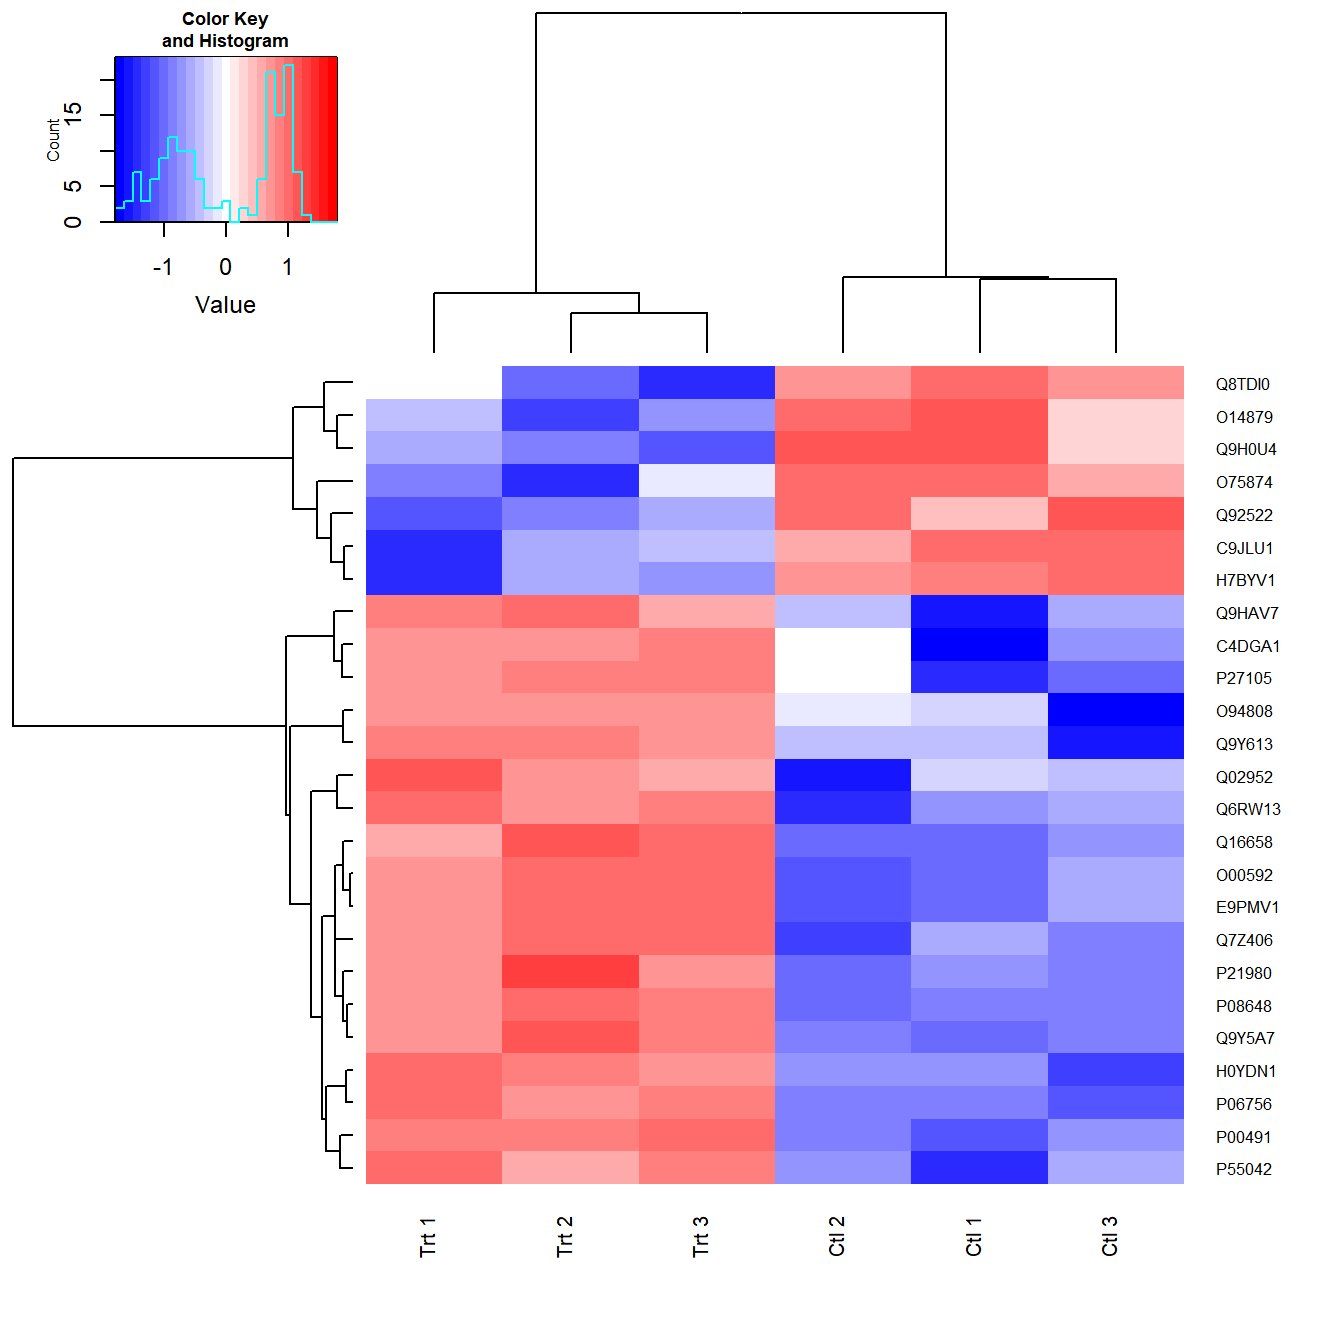
\includegraphics[width=0.8\linewidth]{bspr-workshop-2018_files/figure-latex/heatmap2-1} 

}

\caption{Heatmap created with \texttt{heatmap.2} using the clusters calculated.}\label{fig:heatmap2}
\end{figure}

An alternative and more \texttt{ggplot} style is to use the \texttt{pheatmap} package and
function \citep{R-pheatmap}.

In Figure \ref{fig:pheatmap} \texttt{dat\_scaled} is piped to \texttt{set\_columns} again to
rename the experiments for aesthetic reasons. The output is the piped to
\texttt{pheatmap} which performs the distance and clustering automatically. The only
additional arguements used here are to change the fontsize and create some
breaks in the plot to highlight the clustering.

There is lots more that \texttt{pheatmap} can do in terms of aesthetics, so do explore.



\begin{Shaded}
\begin{Highlighting}[]
\NormalTok{dat_scaled }\OperatorTok\StringTok{ }
\StringTok{  }\CommentTok{# Rename the comlums}
\StringTok{  }\NormalTok{magrittr}\OperatorTok{::}\KeywordTok{set_colnames}\NormalTok{(}\KeywordTok{c}\NormalTok{(}\StringTok{"Ctl 1"}\NormalTok{, }\StringTok{"Ctl 2"}\NormalTok{, }\StringTok{"Ctl 3"}\NormalTok{,}
                                    \StringTok{"Trt 1"}\NormalTok{, }\StringTok{"Trt 2"}\NormalTok{, }\StringTok{"Trt 3"}\NormalTok{)) }\OperatorTok\StringTok{ }
\StringTok{  }\CommentTok{# Plot heatmap}
\StringTok{  }\KeywordTok{pheatmap}\NormalTok{(.,}
           \DataTypeTok{fontsize =} \DecValTok{7}\NormalTok{,}
           \DataTypeTok{cutree_rows =} \DecValTok{2}\NormalTok{, }\CommentTok{# Create breaks in heatmap}
           \DataTypeTok{cutree_cols =} \DecValTok{2}\NormalTok{) }\CommentTok{# Create breaks in heatmap}
\end{Highlighting}
\end{Shaded}

\begin{figure}

{\centering 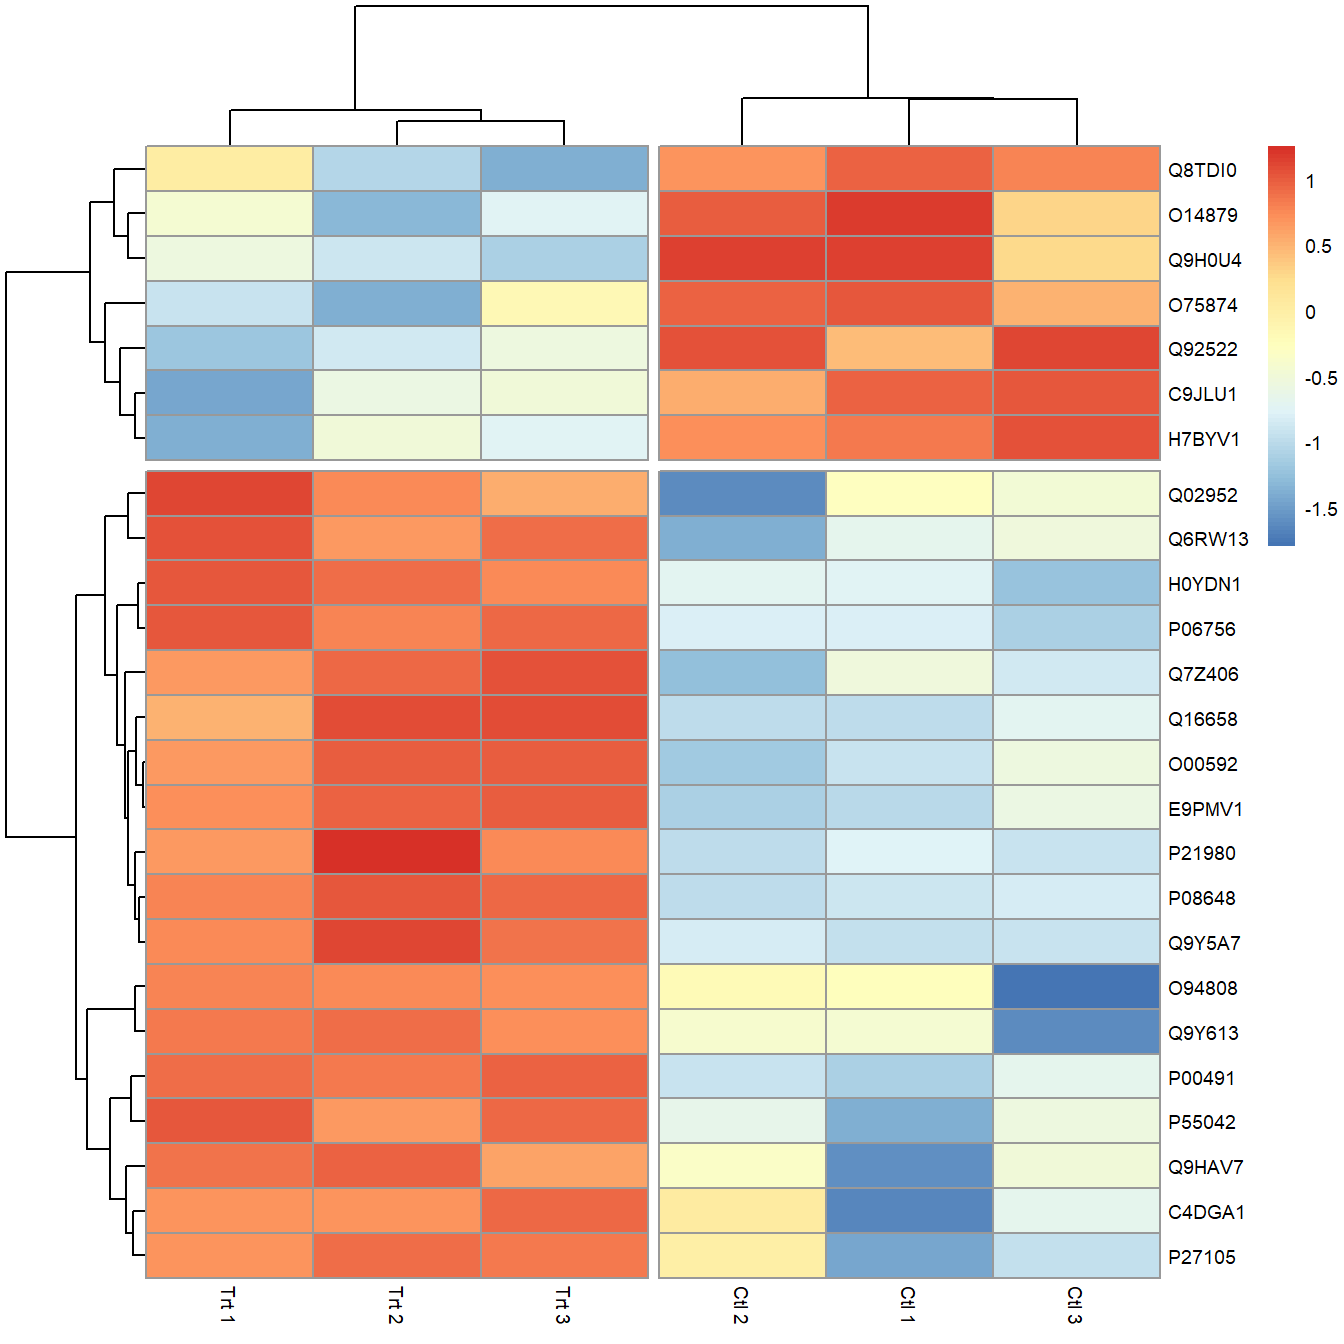
\includegraphics[width=0.8\linewidth]{bspr-workshop-2018_files/figure-latex/pheatmap-1} 

}

\caption{Heatmap created using \texttt{pheatmap} with breaks to highlight clusters.}\label{fig:pheatmap}
\end{figure}

\hypertarget{venn}{%
\section{Venn diagram}\label{venn}}

Another common plot used in proteomics is the Venn diagram. For these I use
the \texttt{VennDiagram} package \citep{R-VennDiagram}.

For example if we wanted to compare the protein identifications found in the
control and treatment sets of our data we could compare the protein accessions
found in each control experiment to see how well they replicate.
To do this we need to transform the data, for example using the following steps:

\begin{enumerate}
\def\labelenumi{\arabic{enumi}.}
\tightlist
\item
  Rather than having variables for the protein concentrations called \texttt{control\_1},
  \texttt{control\_2} etc. in this situation it would make more sense to have a variable
  called \texttt{concentration} and create a new variable for the experiments using the
  column labels, which I'll call \texttt{exp\_type}. Why? By creating a variable with
  the experiment names, we can use \texttt{filter} to easily subset the identified
  proteins in each experiment using our new variable, as we'll see.
\end{enumerate}

This is an example of using the
\texttt{gather} function. The \texttt{key} is the new column we wish to gather the old
column names to, and \texttt{value} is the new column in which the values from the
gathered columns go. I've given the new columns the names \texttt{exp\_type} and \texttt{value}
respectively. We don't want to gather the \texttt{protein\_accession} or
\texttt{protein\_description} columns, so I use \texttt{c()} and use the minus sign to negate
them. These rows get duplicated to match the gathered observations. Hence we
go from 7702 observations of 8 variables, to 46212 observations of 4 variables
when we gather the 6 control and treatment columns.

To do the opposite i.e.~spread one column to many columns, unsuprisingly uses
the function \texttt{spread}. You can read more about both \texttt{gather} and \texttt{spread} in
the \href{http://r4ds.had.co.nz/tidy-data.html\#spreading-and-gathering}{R4DS tidy data chapter}.

\begin{Shaded}
\begin{Highlighting}[]
\CommentTok{# Transform data for Venn diagram to create long table with three columns }
\NormalTok{venn_dat <-}\StringTok{ }\NormalTok{dat }\OperatorTok
\StringTok{  }\CommentTok{# Gather columns according to experiment type to create exp_type }
\StringTok{  }\CommentTok{# and concentration variables. Don't use the protein accession.}
\StringTok{               }\KeywordTok{gather}\NormalTok{(}\DataTypeTok{key =}\NormalTok{ exp_type, }\DataTypeTok{value =}\NormalTok{ concentration, }
                      \OperatorTok{-}\KeywordTok{c}\NormalTok{(protein_accession,protein_description))}

\CommentTok{# Glimpse the gathered data}
\KeywordTok{glimpse}\NormalTok{(venn_dat)}
\end{Highlighting}
\end{Shaded}

\begin{verbatim}
## Observations: 46,212
## Variables: 4
## $ protein_accession   <chr> "VATA_HUMAN_P38606", "RL35A_HUMAN_P18077",...
## $ protein_description <chr> "V-type proton ATPase catalytic subunit A ...
## $ exp_type            <chr> "control_1", "control_1", "control_1", "co...
## $ concentration       <dbl> 0.8114, 0.3672, 2.9815, 0.1424, 1.0748, 0....
\end{verbatim}

\begin{enumerate}
\def\labelenumi{\arabic{enumi}.}
\setcounter{enumi}{1}
\tightlist
\item
  Having transformed the data, we then create three new objects that
  \texttt{filter} the rows for the three control assays using their names, and where
  a concentration was observed using \texttt{!is.na()}. The \texttt{!} means not and \texttt{is.na} tests
  for missing values labelled \texttt{NA}. So read this as
  \emph{where concentration is not a missing value}. The output of filter is piped to
  the dplyr \texttt{pull} function which pulls out the values from the \texttt{protein\_accession}
  column which are stored in the object. These are character vectors, so repeating
  this for all three experiment yields three character vectors of different sizes.
\end{enumerate}

\begin{Shaded}
\begin{Highlighting}[]
\NormalTok{venn_cntl_}\DecValTok{1}\NormalTok{ <-}\StringTok{ }\NormalTok{venn_dat }\OperatorTok\StringTok{ }
\StringTok{  }\KeywordTok{filter}\NormalTok{(exp_type }\OperatorTok{==}\StringTok{ "control_1"} \OperatorTok{&}\StringTok{ }\OperatorTok{!}\KeywordTok{is.na}\NormalTok{(concentration)) }\OperatorTok\StringTok{ }
\StringTok{  }\KeywordTok{pull}\NormalTok{(protein_accession)}

\NormalTok{venn_cntl_}\DecValTok{2}\NormalTok{ <-}\StringTok{ }\NormalTok{venn_dat }\OperatorTok\StringTok{ }
\StringTok{  }\KeywordTok{filter}\NormalTok{(exp_type }\OperatorTok{==}\StringTok{ "control_2"} \OperatorTok{&}\StringTok{ }\OperatorTok{!}\KeywordTok{is.na}\NormalTok{(concentration)) }\OperatorTok\StringTok{ }
\StringTok{  }\KeywordTok{pull}\NormalTok{(protein_accession)}

\NormalTok{venn_cntl_}\DecValTok{3}\NormalTok{ <-}\StringTok{ }\NormalTok{venn_dat }\OperatorTok\StringTok{ }
\StringTok{  }\KeywordTok{filter}\NormalTok{(exp_type }\OperatorTok{==}\StringTok{ "control_3"} \OperatorTok{&}\StringTok{ }\OperatorTok{!}\KeywordTok{is.na}\NormalTok{(concentration)) }\OperatorTok\StringTok{ }
\StringTok{  }\KeywordTok{pull}\NormalTok{(protein_accession)}
\end{Highlighting}
\end{Shaded}

\begin{enumerate}
\def\labelenumi{\arabic{enumi}.}
\setcounter{enumi}{2}
\tightlist
\item
  The three character vectors can be collected into a single object, but as
  they are different lengths, it has to be a \protect\hyperlink{lists}{list object}. Here we use \texttt{list()}
  to create a list of the three character vectors created in step 2. Note that
  I've named the list elements using strings in quotes e.g.~\texttt{"Control\ 1"} this
  allows for a space in the names as I want to use these names on the venn diagram.
\end{enumerate}

\begin{Shaded}
\begin{Highlighting}[]
\CommentTok{# Create a list for plotting}
\NormalTok{venn_list <-}\StringTok{ }\KeywordTok{list}\NormalTok{(}\StringTok{"Control 1"}\NormalTok{ =}\StringTok{ }\NormalTok{venn_cntl_}\DecValTok{1}\NormalTok{,}
                  \StringTok{"Control 2"}\NormalTok{ =}\StringTok{ }\NormalTok{venn_cntl_}\DecValTok{2}\NormalTok{,}
                  \StringTok{"Control 3"}\NormalTok{ =}\StringTok{ }\NormalTok{venn_cntl_}\DecValTok{3}\NormalTok{)}
\end{Highlighting}
\end{Shaded}

\begin{enumerate}
\def\labelenumi{\arabic{enumi}.}
\setcounter{enumi}{3}
\tightlist
\item
  Finally we can plot the venn diagram using the list object\texttt{venn\_list} to
  create a venn diagram object \texttt{prot\_venn} using \texttt{venn.diagram} function from the
  \texttt{VennDiagram} package \citep{R-VennDiagram} and then plotting \texttt{prot\_venn} using
  \texttt{grid.arrange} from the \texttt{gridExtra} package \citep{R-gridExtra}.
\end{enumerate}

I'll leave as an exercise for the reader to look at all the options for
\texttt{venn.diagram} and \texttt{grid.arrange}, but a couple of things to note here are
that you can create three or four way venn diagrams, and if you create
several venn diagram objects, they can be plotted on the same plot using
\texttt{grid\ arrange}. Also here I've added a line to prevent the output of a log file
using \texttt{futile.logger}. You might want these, but generally I don't.



\begin{Shaded}
\begin{Highlighting}[]
\CommentTok{# Prevent the output of a log file}
\NormalTok{futile.logger}\OperatorTok{::}\KeywordTok{flog.threshold}\NormalTok{(futile.logger}\OperatorTok{::}\NormalTok{ERROR, }\DataTypeTok{name =} \StringTok{"VennDiagramLogger"}\NormalTok{)}
\end{Highlighting}
\end{Shaded}

\begin{verbatim}
## NULL
\end{verbatim}

\begin{Shaded}
\begin{Highlighting}[]
\CommentTok{# Create a venn diagram object}
\NormalTok{prot_venn <-}\StringTok{ }\KeywordTok{venn.diagram}\NormalTok{(venn_list,}\OtherTok{NULL}\NormalTok{, }
               \DataTypeTok{col =} \StringTok{"transparent"}\NormalTok{,}
               \DataTypeTok{fill =} \KeywordTok{c}\NormalTok{(}\StringTok{"cornflowerblue"}\NormalTok{, }\StringTok{"green"}\NormalTok{, }\StringTok{"yellow"}\NormalTok{),}
               \DataTypeTok{alpha =} \FloatTok{0.50}\NormalTok{,}
               \DataTypeTok{cex =} \FloatTok{0.8}\NormalTok{,}
               \DataTypeTok{fontfamily =} \StringTok{"sans"}\NormalTok{,}
               \DataTypeTok{fontface =} \StringTok{"bold"}\NormalTok{,}
               \DataTypeTok{cat.col =} \KeywordTok{c}\NormalTok{(}\StringTok{"darkblue"}\NormalTok{, }\StringTok{"darkgreen"}\NormalTok{, }\StringTok{"orange"}\NormalTok{),}
               \DataTypeTok{cat.cex =} \FloatTok{0.8}\NormalTok{,}
               \DataTypeTok{cat.fontfamily =} \StringTok{"sans"}\NormalTok{,}
               \DataTypeTok{margin =} \FloatTok{0.2}\NormalTok{,}
               \DataTypeTok{main =} \StringTok{"Proteins identified in control experiments"}\NormalTok{,}
               \DataTypeTok{main.fontfamily =} \StringTok{"sans"}\NormalTok{,}
               \DataTypeTok{print.mode =} \KeywordTok{c}\NormalTok{(}\StringTok{"raw"}\NormalTok{,}\StringTok{"percent"}\NormalTok{), }\CommentTok{# Show both numbers and percent}
               \DataTypeTok{main.pos =} \KeywordTok{c}\NormalTok{(}\FloatTok{0.5}\NormalTok{,}\FloatTok{0.9}\NormalTok{)}
\NormalTok{  )}

\CommentTok{# Plot the venn diagram using the gridExtra package}
\KeywordTok{grid.arrange}\NormalTok{(}\KeywordTok{gTree}\NormalTok{(}\DataTypeTok{children =}\NormalTok{ prot_venn))}
\end{Highlighting}
\end{Shaded}

\begin{figure}

{\centering 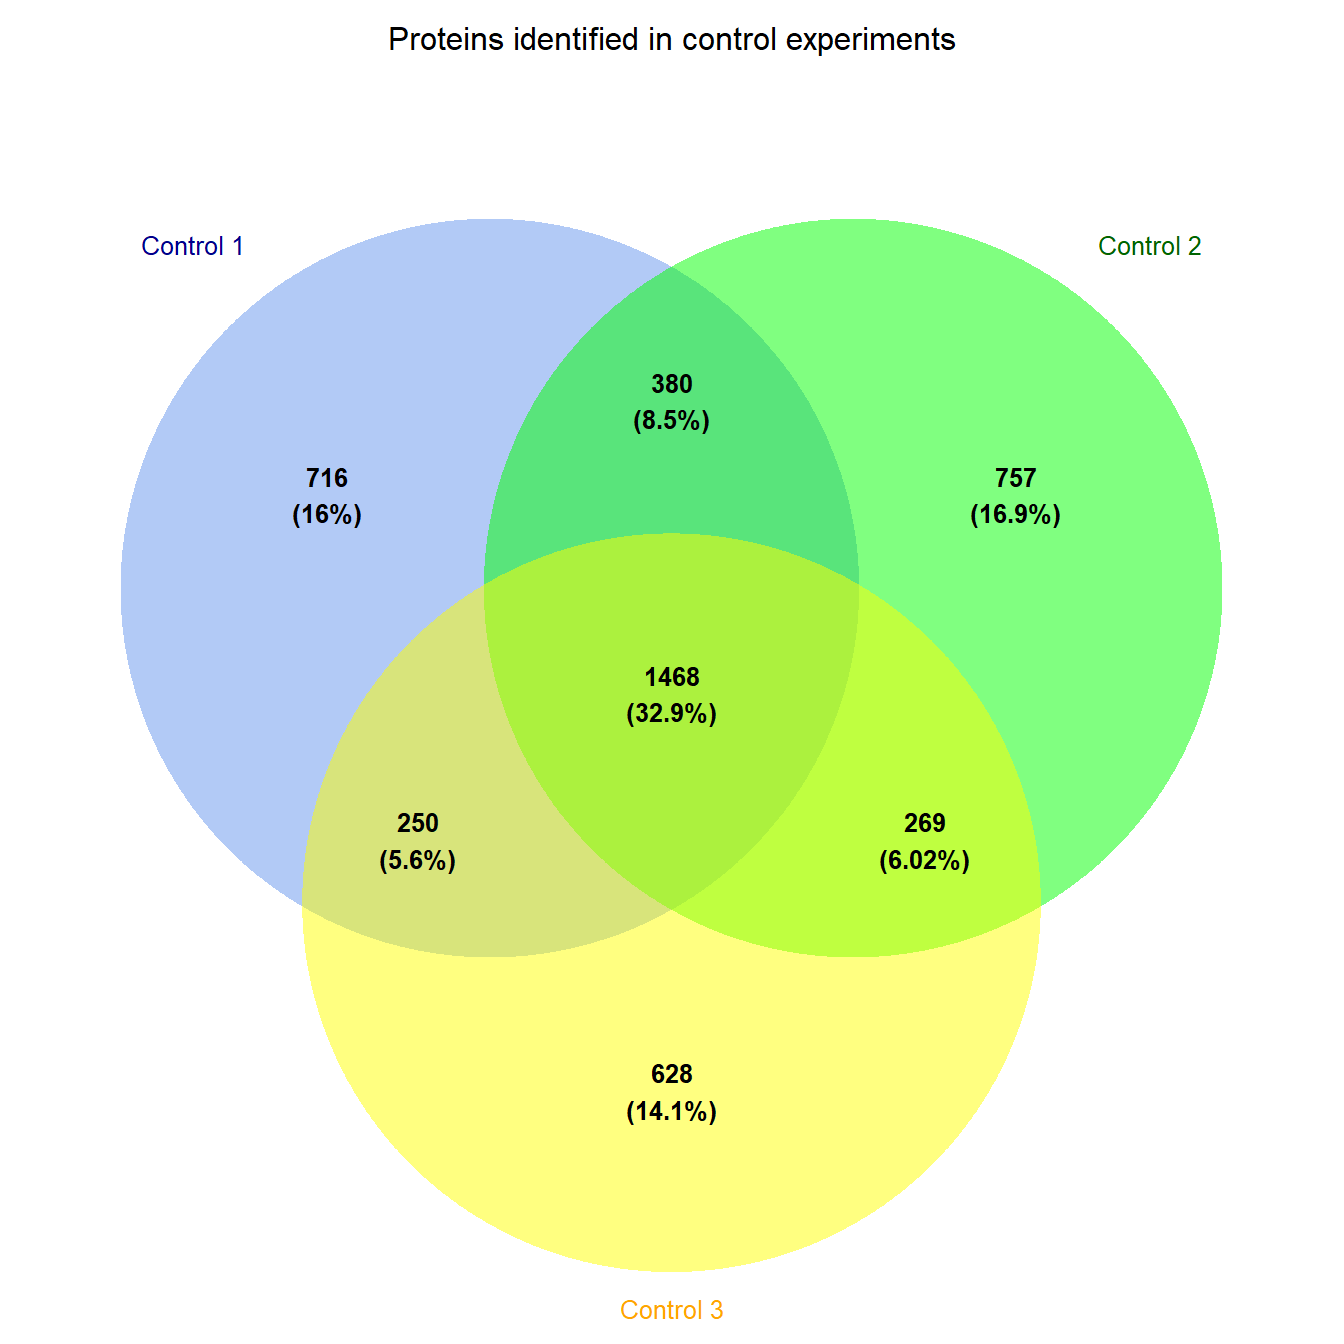
\includegraphics{bspr-workshop-2018_files/figure-latex/venn-plot-1} 

}

\caption{Venn diagram of proteins identified in three control experiments}\label{fig:venn-plot}
\end{figure}

Figure \ref{fig:venn-plot} then shows us that there is a core of around 1500
proteins identified in all three control experiements. You could try something
similar with the treatment experiments.

\hypertarget{peptide-sequence-logos}{%
\section{Peptide sequence logos}\label{peptide-sequence-logos}}

Finally, creating sequence logos from peptides is another common task, especially
if you are doing immunopeptidomics or any situatio where you would like to explore
the fequency of amino acid types at each position in a set of peptide sequences.
The\texttt{ggseqlogo} package enables us to do this \texttt{ggplot2} style \citep{R-ggseqlogo} for
protein, DNA and RNA sequences.

Here using sample data that comes with the ggseqlogo package and illusrated
in the \href{https://omarwagih.github.io/ggseqlogo/}{ggseqlogo tutorial}.

As with the venn diagram, peptide vectors are not generally of equal length
and therefore are collected into a \protect\hyperlink{lists}{list object}. We don't have any
peptides in the example data for the workshop, but the concept of using \texttt{pull}
to extract character vectors was shown in Section \ref{venn}. In this
scenario we'd be extracting character vectors of the peptide sequences and then
collecting them as a named list.

\texttt{ggseqlogo} provides some data \texttt{seqs\_aa} containing a sets of kinase-substrate
phosphorylation sites. This is represented as a named list of character vectors
where the names represent the names of the kinases associated with the
phosphosites.

Below, we load the example data and then the plotting uses the \texttt{ggseqlogo} function
which as with \texttt{ggplot} the first arguement is the data. Other arguements can
be passed either within the function or added using the \texttt{+} operater as per
\texttt{ggplot}.

Here are two examples:

\begin{Shaded}
\begin{Highlighting}[]
\CommentTok{# Load the example data}
\KeywordTok{data}\NormalTok{(ggseqlogo_sample)}

\CommentTok{# Plot the protein sequences with default arguements }
\KeywordTok{ggseqlogo}\NormalTok{(}\DataTypeTok{data =}\NormalTok{ seqs_aa)}
\end{Highlighting}
\end{Shaded}

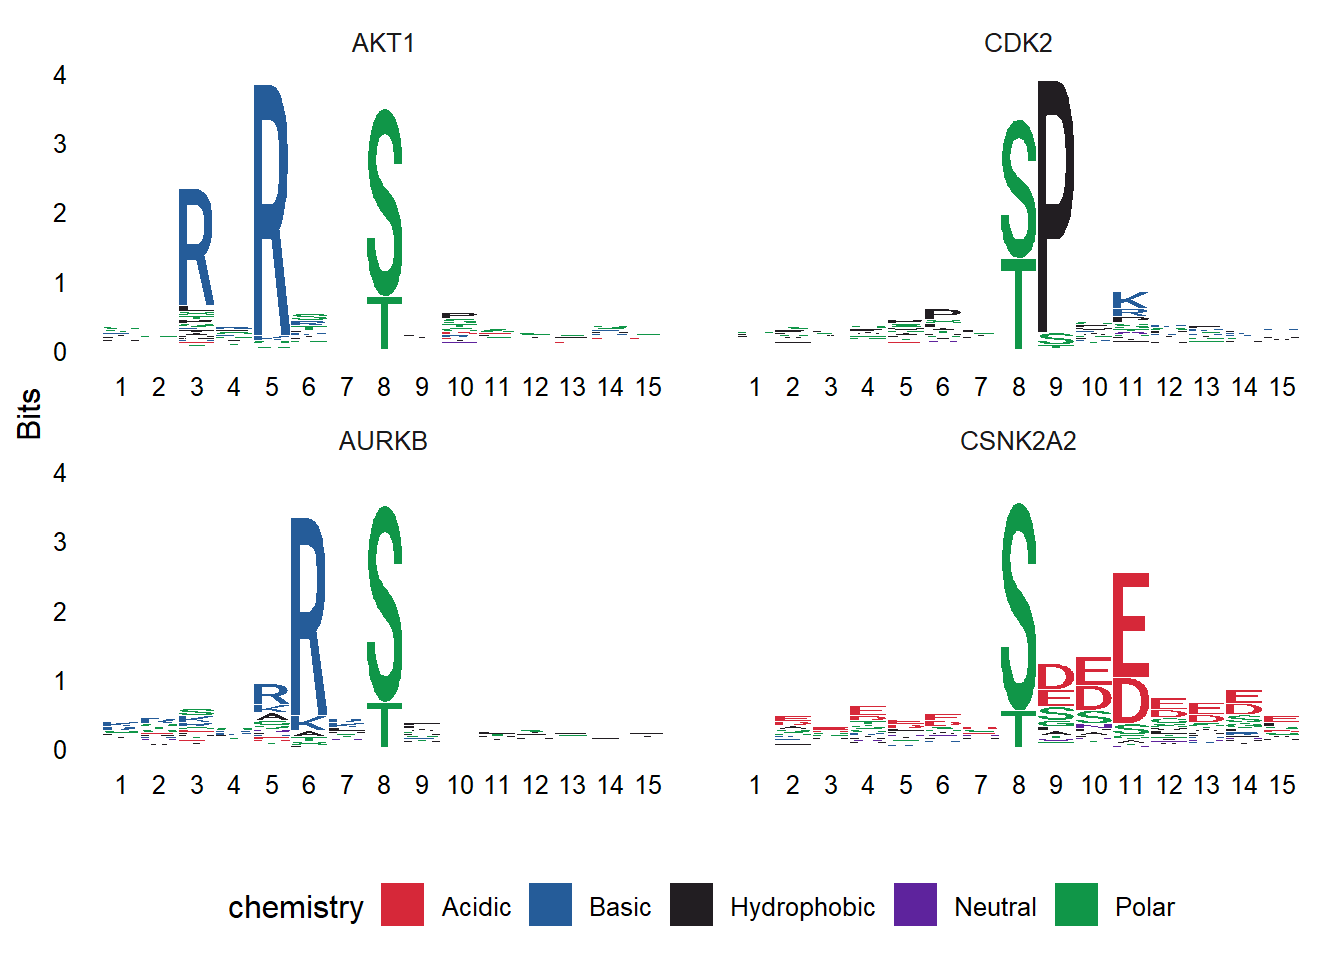
\includegraphics{bspr-workshop-2018_files/figure-latex/ggseqlogo-1.pdf}

\begin{Shaded}
\begin{Highlighting}[]
\CommentTok{# Plot the protein sequences, plotting probability, and change the theme}
\KeywordTok{ggseqlogo}\NormalTok{(}\DataTypeTok{data =}\NormalTok{ seqs_aa, }\DataTypeTok{method =} \StringTok{'prob'}\NormalTok{) }\OperatorTok{+}
\StringTok{  }\KeywordTok{theme_classic}\NormalTok{()}
\end{Highlighting}
\end{Shaded}

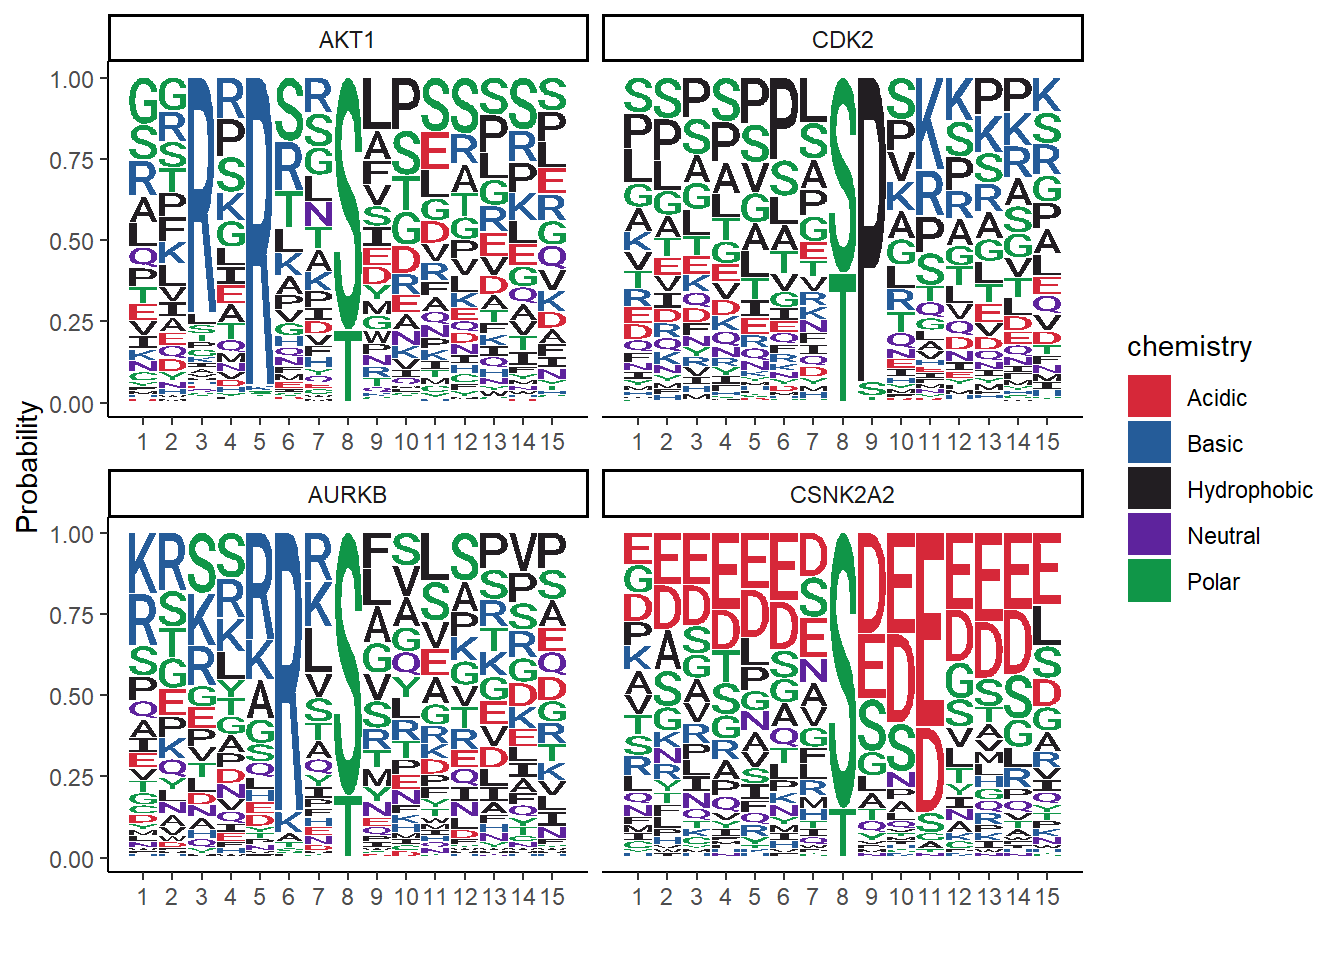
\includegraphics{bspr-workshop-2018_files/figure-latex/ggseqlogo-2.pdf}

\hypertarget{going-further}{%
\chapter{Going further}\label{going-further}}

Here are a few links and suggestions about what else you might like to do with
R.

\hypertarget{export-figs}{%
\section{Exporting figures}\label{export-figs}}

Exporting figures can be done using the following structure:

\begin{Shaded}
\begin{Highlighting}[]
\CommentTok{# Open up a blank plot file, pdf,jpeg etc.}
\OperatorTok{<}\KeywordTok{plot_function}\NormalTok{(}\StringTok{"file"}\NormalTok{,...)}\OperatorTok{>}
\CommentTok{# Write the plot to the file}
\ErrorTok{<}\NormalTok{plot_object}\OperatorTok{>}
\CommentTok{# Close the file}
\KeywordTok{dev.off}\NormalTok{()}
\end{Highlighting}
\end{Shaded}

For example to export the volcano plot from Figure \ref{fig:nice-vplot} to a pdf, we do:

\begin{Shaded}
\begin{Highlighting}[]
\CommentTok{# Open up a blank plot file, pdf,jpeg etc.}
\KeywordTok{pdf}\NormalTok{(}\StringTok{"volcano_plot.pdf"}\NormalTok{)}

\CommentTok{# Write the plot to the file}
\NormalTok{dat_tf }\OperatorTok
\StringTok{  }\CommentTok{# Add a threhold for significant observations}
\StringTok{  }\KeywordTok{mutate}\NormalTok{(}\DataTypeTok{threshold =} \KeywordTok{if_else}\NormalTok{(log_fc }\OperatorTok{>=}\StringTok{ }\DecValTok{2} \OperatorTok{&}\StringTok{ }\NormalTok{log_pval }\OperatorTok{>=}\StringTok{ }\FloatTok{1.3} \OperatorTok{|}
\StringTok{                               }\NormalTok{log_fc }\OperatorTok{<=}\StringTok{ }\DecValTok{-2} \OperatorTok{&}\StringTok{ }\NormalTok{log_pval }\OperatorTok{>=}\StringTok{ }\FloatTok{1.3}\NormalTok{,}\StringTok{"A"}\NormalTok{, }\StringTok{"B"}\NormalTok{)) }\OperatorTok
\StringTok{  }\CommentTok{# Plot with points coloured according to the threshold}
\StringTok{  }\KeywordTok{ggplot}\NormalTok{(}\KeywordTok{aes}\NormalTok{(log_fc,log_pval, }\DataTypeTok{colour =}\NormalTok{ threshold)) }\OperatorTok{+}
\StringTok{  }\KeywordTok{geom_point}\NormalTok{(}\DataTypeTok{alpha =} \FloatTok{0.5}\NormalTok{) }\OperatorTok{+}\StringTok{ }\CommentTok{# Alpha sets the transparency of the points}
\StringTok{  }\CommentTok{# Add dotted lines to indicate the threshold, semi-transparent}
\StringTok{  }\KeywordTok{geom_hline}\NormalTok{(}\DataTypeTok{yintercept =} \FloatTok{1.3}\NormalTok{, }\DataTypeTok{linetype =} \DecValTok{2}\NormalTok{, }\DataTypeTok{alpha =} \FloatTok{0.5}\NormalTok{) }\OperatorTok{+}\StringTok{ }
\StringTok{  }\KeywordTok{geom_vline}\NormalTok{(}\DataTypeTok{xintercept =} \DecValTok{2}\NormalTok{, }\DataTypeTok{linetype =} \DecValTok{2}\NormalTok{, }\DataTypeTok{alpha =} \FloatTok{0.5}\NormalTok{) }\OperatorTok{+}
\StringTok{  }\KeywordTok{geom_vline}\NormalTok{(}\DataTypeTok{xintercept =} \DecValTok{-2}\NormalTok{, }\DataTypeTok{linetype =} \DecValTok{2}\NormalTok{, }\DataTypeTok{alpha =} \FloatTok{0.5}\NormalTok{) }\OperatorTok{+}
\StringTok{  }\CommentTok{# Set the colour of the points}
\StringTok{  }\KeywordTok{scale_colour_manual}\NormalTok{(}\DataTypeTok{values =} \KeywordTok{c}\NormalTok{(}\StringTok{"A"}\NormalTok{=}\StringTok{ "red"}\NormalTok{, }\StringTok{"B"}\NormalTok{=}\StringTok{ "black"}\NormalTok{)) }\OperatorTok{+}
\StringTok{  }\KeywordTok{xlab}\NormalTok{(}\StringTok{"log2 fold change"}\NormalTok{) }\OperatorTok{+}\StringTok{ }\KeywordTok{ylab}\NormalTok{(}\StringTok{"-log10 p-value"}\NormalTok{) }\OperatorTok{+}\StringTok{ }\CommentTok{# Relabel the axes}
\StringTok{  }\KeywordTok{theme_minimal}\NormalTok{() }\OperatorTok{+}\StringTok{ }\CommentTok{# Set the theme}
\StringTok{  }\KeywordTok{theme}\NormalTok{(}\DataTypeTok{legend.position=}\StringTok{"none"}\NormalTok{) }\CommentTok{# Hide the legend}

\CommentTok{# Close the file}
\KeywordTok{dev.off}\NormalTok{()}
\end{Highlighting}
\end{Shaded}

If I had saved the plot to an object called \texttt{vplot} I would call that object
instead of making the plot using \texttt{dat\_tf} as shown here.

\href{https://www.stat.berkeley.edu/classes/s133/saving.html}{Here} is a general
guide to the various formats you can export to.

Alternatively, if you are working in \texttt{ggplot} you can use the \texttt{ggsave} function
as described in \href{http://r4ds.had.co.nz/graphics-for-communication.html\#saving-your-plots}{R4DS 28.7}.

\begin{Shaded}
\begin{Highlighting}[]
\CommentTok{# Plot}
\NormalTok{dat_tf }\OperatorTok
\StringTok{  }\CommentTok{# Add a threhold for significant observations}
\StringTok{  }\KeywordTok{mutate}\NormalTok{(}\DataTypeTok{threshold =} \KeywordTok{if_else}\NormalTok{(log_fc }\OperatorTok{>=}\StringTok{ }\DecValTok{2} \OperatorTok{&}\StringTok{ }\NormalTok{log_pval }\OperatorTok{>=}\StringTok{ }\FloatTok{1.3} \OperatorTok{|}
\StringTok{                               }\NormalTok{log_fc }\OperatorTok{<=}\StringTok{ }\DecValTok{-2} \OperatorTok{&}\StringTok{ }\NormalTok{log_pval }\OperatorTok{>=}\StringTok{ }\FloatTok{1.3}\NormalTok{,}\StringTok{"A"}\NormalTok{, }\StringTok{"B"}\NormalTok{)) }\OperatorTok
\StringTok{  }\CommentTok{# Plot with points coloured according to the threshold}
\StringTok{  }\KeywordTok{ggplot}\NormalTok{(}\KeywordTok{aes}\NormalTok{(log_fc,log_pval, }\DataTypeTok{colour =}\NormalTok{ threshold)) }\OperatorTok{+}
\StringTok{  }\KeywordTok{geom_point}\NormalTok{(}\DataTypeTok{alpha =} \FloatTok{0.5}\NormalTok{) }\OperatorTok{+}\StringTok{ }\CommentTok{# Alpha sets the transparency of the points}
\StringTok{  }\CommentTok{# Add dotted lines to indicate the threshold, semi-transparent}
\StringTok{  }\KeywordTok{geom_hline}\NormalTok{(}\DataTypeTok{yintercept =} \FloatTok{1.3}\NormalTok{, }\DataTypeTok{linetype =} \DecValTok{2}\NormalTok{, }\DataTypeTok{alpha =} \FloatTok{0.5}\NormalTok{) }\OperatorTok{+}\StringTok{ }
\StringTok{  }\KeywordTok{geom_vline}\NormalTok{(}\DataTypeTok{xintercept =} \DecValTok{2}\NormalTok{, }\DataTypeTok{linetype =} \DecValTok{2}\NormalTok{, }\DataTypeTok{alpha =} \FloatTok{0.5}\NormalTok{) }\OperatorTok{+}
\StringTok{  }\KeywordTok{geom_vline}\NormalTok{(}\DataTypeTok{xintercept =} \DecValTok{-2}\NormalTok{, }\DataTypeTok{linetype =} \DecValTok{2}\NormalTok{, }\DataTypeTok{alpha =} \FloatTok{0.5}\NormalTok{) }\OperatorTok{+}
\StringTok{  }\CommentTok{# Set the colour of the points}
\StringTok{  }\KeywordTok{scale_colour_manual}\NormalTok{(}\DataTypeTok{values =} \KeywordTok{c}\NormalTok{(}\StringTok{"A"}\NormalTok{=}\StringTok{ "red"}\NormalTok{, }\StringTok{"B"}\NormalTok{=}\StringTok{ "black"}\NormalTok{)) }\OperatorTok{+}
\StringTok{  }\KeywordTok{xlab}\NormalTok{(}\StringTok{"log2 fold change"}\NormalTok{) }\OperatorTok{+}\StringTok{ }\KeywordTok{ylab}\NormalTok{(}\StringTok{"-log10 p-value"}\NormalTok{) }\OperatorTok{+}\StringTok{ }\CommentTok{# Relabel the axes}
\StringTok{  }\KeywordTok{theme_minimal}\NormalTok{() }\OperatorTok{+}\StringTok{ }\CommentTok{# Set the theme}
\StringTok{  }\KeywordTok{theme}\NormalTok{(}\DataTypeTok{legend.position=}\StringTok{"none"}\NormalTok{) }\CommentTok{# Hide the legend}

\CommentTok{# Use ggsave to save the plot as pdf}
\KeywordTok{ggsave}\NormalTok{(}\StringTok{"volcano_plot.pdf"}\NormalTok{, }\DataTypeTok{width =} \DecValTok{20}\NormalTok{, }\DataTypeTok{height =} \DecValTok{20}\NormalTok{, }\DataTypeTok{units =} \StringTok{"cm"}\NormalTok{)}
\end{Highlighting}
\end{Shaded}

\hypertarget{exporting-data}{%
\section{Exporting data}\label{exporting-data}}

There is a \href{https://cran.r-project.org/doc/manuals/r-release/R-data.html}{full manual for the import and export of data} in R.
However here are few pointers:

\hypertarget{writing-to-a-file}{%
\subsection{Writing to a file}\label{writing-to-a-file}}

One of the most portables way to share data is by writing to a csv file. These
files can be opened in many programs. The tidyverse package contains two
functions for csv files, \texttt{write\_csv} and for Excel \texttt{write\_excel\_csv}. The
latter form adds a bit of metadata that tells Excel about the file encoding.
See \href{http://r4ds.had.co.nz/data-import.html\#writing-to-a-file}{R4DS writing to a file}.

For example to write a csv file of \texttt{dat\_tf} to a file called
\texttt{04072018\_transformed\_data.csv} to our working directory for sharing
with a colleague using excel, the code is of the form
\texttt{\textless{}function\textgreater{}(\textless{}r-object\textgreater{},"filename")} like so:

\begin{Shaded}
\begin{Highlighting}[]
\KeywordTok{write_excel_csv}\NormalTok{(dat_tf,}\StringTok{"04072018_transformed_data.csv"}\NormalTok{)}
\end{Highlighting}
\end{Shaded}

Note that the file name is a string and is in quotes.

\hypertarget{for-r}{%
\subsection{For R}\label{for-r}}

If you are exporting data to use yourself in R, the custom \texttt{.rds} format is a
good choice and preserves the R structure.

In the tidyverse \texttt{write\_rds} follows the same structure as \texttt{write\_csv}.

You can read back in using \texttt{read\_rds}.

\hypertarget{joining-the-r-community}{%
\section{Joining the R community}\label{joining-the-r-community}}

It's worth joining the \href{https://community.rstudio.com/}{RStudio Community} and
following community members on Twitter such as \href{https://twitter.com/JennyBryan}{Jenny Bryan}, \href{https://twitter.com/hadleywickham}{Hadley Wickham}, \href{https://twitter.com/xieyihui}{Yihui Xie}, \href{https://twitter.com/dataandme}{Mara Averick},
\href{https://twitter.com/drob}{David Robinson}
and \href{https://twitter.com/juliasilge}{Julia Silge}.

I would not reccomend DataCamp due to their \href{https://juliasilge.com/blog/datacamp-misconduct/}{misconduct}.

And \href{https://swirlstats.com/}{swirl} is free.

\hypertarget{communication-creating-reports-presentations-and-websites}{%
\section{Communication: creating reports, presentations and websites}\label{communication-creating-reports-presentations-and-websites}}

\href{https://rmarkdown.rstudio.com/lesson-1.html}{R Markdown} \citep{R-rmarkdown} enables us to do
\href{https://en.wikipedia.org/wiki/Literate_programming}{literate programming}, saving time as we can create analysis, reports, dashboards or web apps at the same time
as writing code. R Markdown can use multiple programming languages.
See also \href{http://r4ds.had.co.nz/r-markdown.html}{R4DS R Markdown} and
\href{http://r4ds.had.co.nz/r-markdown-formats.html}{R4DS R Markdown formats} and
the \href{https://bookdown.org/yihui/rmarkdown/}{R Markdown: The Definitive Guide}.

As linked in Section \ref{viz} Claus Wilke has written a very nice guide to
visualising data using R cvisualising data using R called
\href{http://serialmentor.com/dataviz/index.html}{Fundamentals of Data Visualization}
which is very helpful when it comes to thinking about how to best create figures
for a report, poster or presentation.

You can use \href{https://bookdown.org/yihui/blogdown/}{blogdown} to build websites.
I created this guide to \href{http://ab604.github.io/docs/website_bookdown/}{buidling an academic website with blogdown}.

\hypertarget{using-bookdown-to-write-a-thesis-dissertaion}{%
\subsection{Using bookdown to write a thesis dissertaion}\label{using-bookdown-to-write-a-thesis-dissertaion}}

I used the bookdown package to create these materials \citep{R-bookdown} and you can
use it to write a thesis dissertaion, as detailed very nicely in this blog by
\href{https://eddjberry.netlify.com/post/writing-your-thesis-with-bookdown/}{Edd Berry}.

\hypertarget{machine-learning}{%
\section{Machine Learning}\label{machine-learning}}

If you are interested in machine learning, then \href{https://tensorflow.rstudio.com/}{TensorFlow} is a good place to start, for
example Leon Eyrich Jessen's \href{https://tensorflow.rstudio.com/blog/dl-for-cancer-immunotherapy.html}{Deep Learning for Cancer Immunotherapy} tutorial.

\hypertarget{version-control}{%
\section{Version control}\label{version-control}}

Another thing you may wish to consider is version control, \emph{``a system that records changes to a file or set of files over time so that you can recall specific versions later''.}

To get started, have a look at these \href{https://speakerdeck.com/alicebartlett/git-for-humans}{slides by Alice Bartlett} and check out the \href{https://support.rstudio.com/hc/en-us/articles/200532077-Version-Control-with-Git-and-SVN}{Rstudio version control guide}.

\bibliography{packages.bib,book.bib}


\end{document}
